\documentclass{dissertation}

%%% MY PACKAGE
\usepackage{blindtext} % provide \blindtext, \Blindtext
% \usepackage{libertine} % nice font
% % ==  mathematical fonts ==
% \usepackage{ccfonts}  % mathematical fonts
% \usepackage[T1]{fontenc}  % mathematical fonts
% \renewcommand{\rmdefault}{cmr}% cmr = Computer Modern Roman
% % ==  mathematical fonts ==

%%% DEFAULT PACKAGE
\usepackage{amsmath,mathtools,empheq}
\usepackage{amsthm}
\usepackage{thmtools}
\usepackage{thm-restate}
\declaretheorem[%
    name=Rationale,
    refname={Rationale,Rationales},
    Refname={Rationale,Rationales}
]{rationale}
\declaretheorem[%
    name={Security Claim},
    numbered={unless unique},
]{secclaim}

\usepackage{longtable}
\usepackage{pdflscape}
\usepackage{enumitem}

%% COLORS %%

\definecolor{RoyalBlue}{cmyk}{1,0.5,0,0}
\definecolor{Black}{cmyk}{0,0,0,0}
\definecolor{alertred}{rgb}{0.80,0.12,0.12}
\definecolor{linkgreen}{RGB}{0,166,0}


\newrobustcmd*{\fullfullcite}{%
    \AtNextCite{%
        \AtEachCitekey{%
            \defcounter{maxnames}{99}%
            \DeclareNameAlias{labelname}{given-family}%
        }%
    }%
    \fullcite
}

%% IMAGE AS SYMBOL

% % set the Bison QED symbol
% \renewcommand{\qed}{%
% \leavevmode\unskip\penalty9999 \hbox{}\nobreak\hfill%
% \quad\hbox{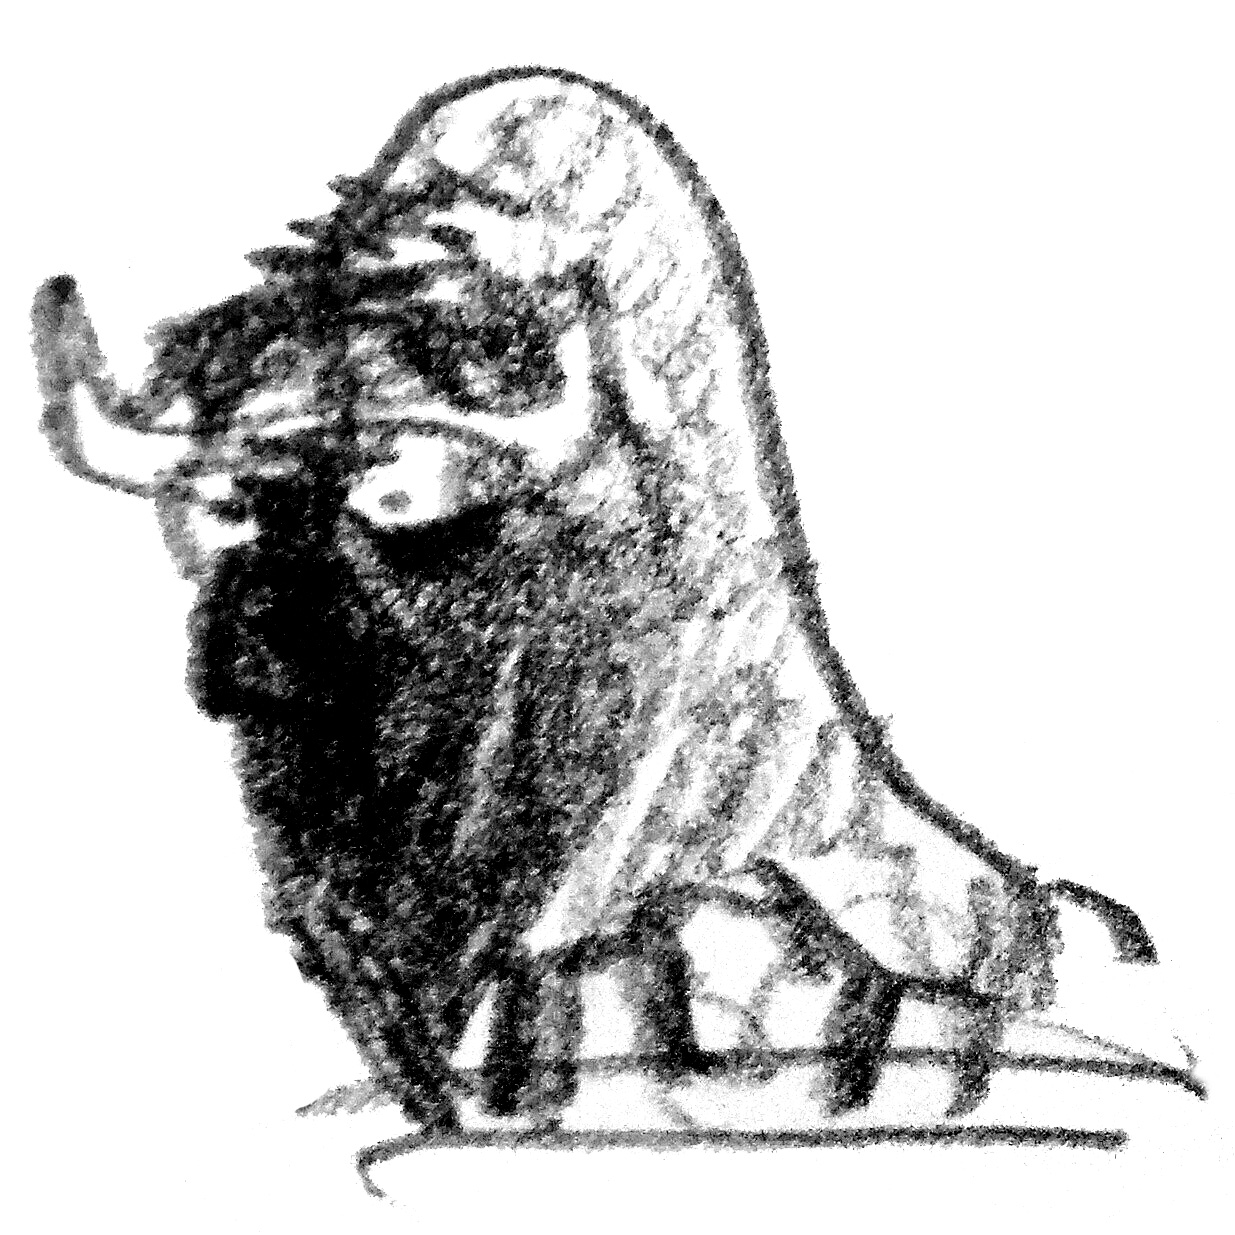
\includegraphics[height=1em]{bison/bison-qed.jpg}}}

\newcommand{\cpother}[1]{{\color{BlueGreen} #1}}
\newcommand{\cpmine}[1]{{\color{GreenYellow} #1}}

% --- my abbreviation ---------------------------------------------------------
\newcommand{\imgsrc}[1]{Image courtesy of #1}
\newcommand{\cfr}[1]{\Cf/ #1}

% --- math models -------------------------------------------------------------
\newcommand{\echoModelFreq}{\ensuremath{
    H_{ij}(f_k) = \sum_{\idxEch=0}^{\numEchs}
        \frac{\absCoeff_{ij}^r}{4 \pi \speedOfSound \tau_{ij}^r}
        \cste^{- \csti 2 \pi k \Fs \tau_{ij}^r / F}}}

\newcommand{\sumEcho}{\ensuremath{\sum_{\idxEch=0}^{\numEchs}}}
\newcommand{\echoModelTimeSimple}[1]{\ensuremath{\sumEcho \alpha_{#1}^{(r)} \delta(t - \tau_{#1}^{(r)})}}
\newcommand{\alltaus}[1]{\ensuremath{\{\tau_{#1}^{(r)}\}_{#1,r}}}
\newcommand{\allalphas}[1]{\ensuremath{\{\alpha_{#1}^{(r)}\}_{#1,r}}}

\newcommand{\icon}[1]{\raisebox{-.1\height}{\includegraphics[height=3ex]{#1}}}
\newcommand{\chaosIcon}{\icon{figures/blaster/chaos.png}}
% --- correct bad hyphenation
\hyphenation{op-tical net-works semi-conduc-tor}

% --- Algos and Methods names:
\newcommand{\mirage}{\textsc{Mirage}}
\newcommand{\separake}{\textsc{Separake}}
\newcommand{\brioche}{\textsc{Brioche}}
\newcommand{\blaster}{\textsc{Blaster}}
\newcommand{\blasterr}{\textsc{Blaster2}}
\newcommand{\lantern}{\textsc{Lantern}}
\newcommand{\dechorate}{d'\textsc{Echorate}}

%----------------
\usepackage{pgffor}
% for math stuff
\foreach \x in {a,...,z}{
  % mathbf
  \expandafter\xdef\csname bf\x \endcsname{\noexpand\ensuremath{\noexpand\mathbf{\x}}}
  % Bold symbol
  \expandafter\xdef\csname bs\x \endcsname{\noexpand\ensuremath{\noexpand\boldsymbol{\x}}}
  % Typewriter
  \expandafter\xdef\csname tt\x \endcsname{\noexpand\ensuremath{\noexpand\mathtt{\x}}}
}

\foreach \x in {A,...,Z}{
%   % Bold symbol -- bold
  \expandafter\xdef\csname bs\x \endcsname{\noexpand\ensuremath{\noexpand\boldsymbol{\x}}}
%   % mathbf -- bold
  \expandafter\xdef\csname bf\x \endcsname{\noexpand\ensuremath{\noexpand\mathbf{\x}}}
%   % mathbb -- blackboard-bold for uppercase letters and lowercase ( for sets )
  \expandafter\xdef\csname bb\x \endcsname{\noexpand\ensuremath{\noexpand\mathbb{\x}}}
%   % mathds -- ???
  \expandafter\xdef\csname ds\x \endcsname{\noexpand\ensuremath{\noexpand\mathds{\x}}}
%   % mathfrak -- gothic
  \expandafter\xdef\csname fk\x \endcsname{\noexpand\ensuremath{\noexpand\mathfrak{\x}}}
%   % mathfrak -- curly
  \expandafter\xdef\csname scr\x \endcsname{\noexpand\ensuremath{\noexpand\mathscr{\x}}}
%   % mathcal -- calligraphy
  \expandafter\xdef\csname cal\x \endcsname{\noexpand\ensuremath{\noexpand\mathcal{\x}}}
}

% --- Math Notation
% math
\newcommand{\Ii}{\ensuremath{\imath}}
% \newcommand{\cstj}{\ensuremath{\jmath}}
\newcommand{\R}{\ensuremath{\bbR}}
\newcommand{\N}{\ensuremath{\bbN}}
\newcommand{\Z}{\ensuremath{\bbZ}}
% indexing
\newcommand{\idxSrc}{\ensuremath{j}}
\newcommand{\idxMic}{\ensuremath{i}}
\newcommand{\idxEch}{\ensuremath{r}}
\newcommand{\numSrcs}{\ensuremath{J}}
\newcommand{\numMics}{\ensuremath{I}}
\newcommand{\numEchs}{\ensuremath{R}}
% geometry
\newcommand{\positionMicrophone}{\ensuremath{\underline{\bfx}}}
\newcommand{\positionSource}{\ensuremath{\underline{\bfs}}}
\newcommand{\positionSurface}{\ensuremath{\underline{\bfp}}}
\newcommand{\pos}{\ensuremath{\bfr}}
\newcommand{\coordinatePermutation}{\ensuremath{\bfR}}
\newcommand{\distMicSrc}{\ensuremath{r}}
\newcommand{\distMicMic}{\ensuremath{d}}
% signal model
\newcommand{\src}{\ensuremath{s}}
\newcommand{\mic}{\ensuremath{x}}
\newcommand{\mics}{\ensuremath{\bsx}}
\newcommand{\img}{\ensuremath{c}}
\newcommand{\imgs}{\ensuremath{\bsc}}
\newcommand{\spat}{\ensuremath{\boldsymbol{\Xi}}}
\newcommand{\master}{\ensuremath{\boldsymbol{\Upsilon}}}
\newcommand{\contRecordedSignal}{\ensuremath{x}}
\newcommand{\contMicrophoneSignal}{\contRecordedSignal}
\newcommand{\contSource}{\ensuremath{s}}
\newcommand{\contFilter}{\ensuremath{h}}
\newcommand{\contFilterHat}{\widehat{\contFilter}}
\newcommand{\contRIR}{\contFilter}
\newcommand{\contNoise}{\ensuremath{n}}
\newcommand{\disRecordedSignal}{\bfx}
\newcommand{\disFilter}{\bfh}
\newcommand{\disFilterHat}{\widehat{\disFilter}}
\newcommand{\RecordedSignalDFT}{\bfX}

% (room) acoustics
\newcommand{\speedOfSound}{\ensuremath{c}}
\newcommand{\cair}{\ensuremath{\speedOfSound_\text{air}}}
\newcommand{\temperature}{\ensuremath{T}}
\newcommand{\rhumidity}{\ensuremath{H}}
\newcommand{\forceVec}{\ensuremath{\bsF}}
\newcommand{\velocity}{\ensuremath{\bsv}}
\newcommand{\pressure}{\ensuremath{p}}
\newcommand{\Pressure}{\ensuremath{P}}
\newcommand{\flux}{\ensuremath{\bsq}}
\newcommand{\density}{\ensuremath{\rho}}
\newcommand{\densityEq}{\density_0}
\newcommand{\mass}{\ensuremath{m}}
\newcommand{\volumeUnit}{\ensuremath{\nu}}
\newcommand{\surface}{\ensuremath{S}}
\newcommand{\volume}{\ensuremath{\calV}}
\newcommand{\impedence}{\ensuremath{Z}}
\newcommand{\impedenceAir}{\ensuremath{\impedence_\text{air}}}
\newcommand{\absCoeff}{\ensuremath{\alpha}}
\newcommand{\reflCoeff}{\ensuremath{\beta}}
\newcommand{\boundariesConditions}{\ensuremath{\calB}}
\newcommand{\wavelength}{\ensuremath{\lambda}}
\newcommand{\ntuple}{\ensuremath{\bsm}}

\newcommand{\depSpaceTime}{\ensuremath{\kparen{\positionMicrophone, t}}}
\newcommand{\pressureSpaceTime}{\ensuremath{\pressure\depSpaceTime}}

% signal processing
\newcommand{\error}{\ensuremath{{\varepsilon}}}
\newcommand{\filterLength}{\ensuremath{{L}}}
\newcommand{\Ts}{\ensuremath{T_s}}
\newcommand{\Fs}{\ensuremath{F_s}}
\newcommand{\zeroVect}{\ensuremath{\mathbf{0}}}
\newcommand{\rir}{\ensuremath{h}}
\newcommand{\rirFreq}{\ensuremath{H}}
\newcommand{\rirs}{\ensuremath{\bsh}}
\newcommand{\rtf}{\ensuremath{\tilde{\rir}}}
\newcommand{\rtfs}{\ensuremath{\tilde{\rirs}}}
\newcommand{\ild}{\ensuremath{\mathtt{ILD}}}
\newcommand{\ipd}{\ensuremath{\mathtt{IPD}}}

% math vars and constant
\newcommand{\spike}[1]{\delta_{#1}}
\newcommand{\opObs}{\calA}
\newcommand{\thr}{\tau_\text{max}}
\newcommand{\algoBraire}{BLASTER}
\newcommand{\algoBsn}{BSN}
\newcommand{\algoCrocco}{IL1C}

% variable
\newcommand{\RT}{\ensuremath{\mathtt{RT}_{60}}}
\newcommand{\DRR}{\ensuremath{\mathtt{DRR}}}
\newcommand{\DER}{\ensuremath{\mathtt{DER}}}
\newcommand{\SNR}{\ensuremath{\mathtt{SNR}}}
\newcommand{\dsetValid}{$\mathbf{\mathcal{D}}^{\:\text{(valid)}}$}
\newcommand{\dsetSNR}{$\mathbf{\mathcal{D}}^{\:\SNR}$}
\newcommand{\dsetRT}{$\mathbf{\mathcal{D}}^{\:\RT}$}

% --- Other (constant)
\newcommand{\const}{\ensuremath{\text{\textit{const.}}}}

\newcommand{\idealLowPassFilter}{\phi}
\newcommand{\disRadonMeasure}{\calM(\Theta)}
\newcommand{\posDisRadonMeasure}{\calM_+(\Theta)}

% \newcommand{\m1}{\mathbf{m}_1}
% \newcommand{\m2}{\mathbf{m}_2}
% \newcommand{\s}{{\mathbf s}}
% \newcommand{\params}{\mathbf{\theta}}

% --- Quantities names

% --- Mathematical Delimiters

% % syntactically named delimiters
% \newdelimcommand{ceil}{\lceil}{\rceil}
% \newdelimcommand{floor}{\lfloor}{\rfloor}
% \newdelimcommand{angles}{\langle}{\rangle}
% \newdelimcommand{parens}{\lparen}{\rparen}
% \newdelimcommand{bracket}{[}{]}
% \newdelimcommand{braces}{\lbrace}{\rbrace}
% \newdelimcommand{verts}{\lvert}{\rvert}
% \newdelimcommand{Verts}{\lVert}{\rVert}

% % semantically named delimiters
\newcommand{\set}[1]{\kbrace{#1}}
% \newcommand{\abs}{\verts}
% \newcommand{\size}{\verts}
\newcommand{\abs}[1]{\kvbar{#1}}
\newcommand{\norm}[1]{\kvvbar{#1}}
\newcommand{\normTV}[1]{\ensuremath{\norm{#1}_{\mathtt{TV}}}}
% \newcommand{\tuple}{\angles}
% \newcommand{\iprod}{\angles}

% % Automagic `such that' for set comprehension. Inside an automagic
% % delimiter command, the vertical bar will resize appropriately
% % Example:
% %   \set{ x \in W \given x > 0 }
\newcommand{\given}{\;\mdelim\vert\;}


% --- Math operators
\DeclareMathOperator*{\fourierTrans}{\scrF}
\DeclareMathOperator*{\discreteFT}{\bfF}
\DeclareMathOperator*{\divergence}{\nabla\cdot}
\DeclareMathOperator*{\dirac}{\delta}
\newcommand{\average}{\operatornamewithlimits{average}}

% --- Mathematical operators and function
\newcommand{\conv}{\ast}
\newcommand{\diracOf}[1]{\dirac\kparen{#1}}
\DeclareMathOperator*{\phase}{\angle}
\newcommand{\phaseOf}[1]{\phase{#1}}
\newcommand{\magnitudeOf}[1]{\abs{#1}}
\newcommand{\powerOf}[1]{\abs{#1}^2}


% other definition
\newcommand{\myeq}{\mathrel{\overset{\makebox[0pt]{\mbox{\normalfont\tiny\sffamily def}}}{=}}}
\newcommand{\mathspace}{\hspace{1em}}

%%% FILE ORGANIZATION
% \graphicspath{{./figures/}{./tikzpictures/}}
% \pgfplotsset{%
%     table/search path={./figures/plots/},
% }
\bibliography{contents/bibliography/abbrev3,
              contents/bibliography/crypto,
              contents/bibliography/references}


\title{Hunting Acoustic Echoes for Auditory Scene Analysis}
\author{Diego DI CARLO}
\date{\today}

\begin{document}
\frontmatter{}


% % front matter / titelei
% recto: halftitlepage / schmutztitelseite, vortitel
\thispagestyle{empty}
{
    \begin{fullwidth}
        \centering
        \hphantom{.}
        \vfill
        {\Huge
            Security Arguments and\\
            Tool-based Design of Block Ciphers
        }
        \vfill
        \vfill
    \end{fullwidth}
}

\clearpage{}

% verso: frontispiece / frontiszipzseite, vakatseite
% dedication
\cleardoublepage{}

% recto: titlepage / titelblatt, innentitel
\thispagestyle{empty}
{
    \calccentering{\unitlength}
    \begin{adjustwidth*}{\unitlength}{-\unitlength}
        \raggedleft{}
        {\Huge\color{Burgundy}%
        Security Arguments and\\
        Tool-based Design of Block Ciphers}\\[\baselineskip]
        {\LARGE%
        Dissertation Thesis}\\[0.2\textheight]
        {\huge%
        Friedrich Wiemer}\\[\baselineskip]
        {\LARGE%
        16th~August 2019}
        \vfill
        \vfill
        {\large%
        Submitted in partial fulfillment of the requirements\\
        for the degree of Doktor der Naturwissenschaften\\[\baselineskip]% (Dr.\ rer.\ nat.)\\[\baselineskip]

        to the\\[\baselineskip]

        Faculty of Mathematics\\
        at Ruhr-Universität Bochum\\[2\baselineskip]
        %Vorgelegt zur Erlangung des\\
        %Doktorgrades der Naturwissenschaften\\
        %an der Fakultät der Mathematik\\
        %der Ruhr-Universität Bochum\\[2\baselineskip]

        \begin{minipage}{0.5\textwidth}
        \begin{tabular}{lr}
            1st\hspace{4pt} Reviewer & Prof.\ Dr. Gregor Leander\\
            2nd Reviewer & Prof.\ Dr.\; Alexander May
        \end{tabular}
        \end{minipage}
        \hspace*{36pt}
        %}\hspace*{-8pt}

        %\vspace{2\baselineskip}
        %Datum der Disputation: 13.\ Dezember 2019
        \vfill
        }
        \vspace*{\baselineskip}
    \end{adjustwidth*}
}

\clearpage{}

% verso: colophon / impressum
\thispagestyle{empty}
\hphantom{.}
\vfill

\section*{Imprint}

\textit{Security Arguments and Tool-based Design of Block Ciphers}\\
Copyright \textcopyright{} 2019 by \theauthor{}.\\
All rights reserved. Printed in Germany.\\
Published by the Ruhr-Universität Bochum, Bochum, Germany.

\section*{Colophon}

This thesis was typeset using \LaTeX{} and the \texttt{memoir} documentclass.
It is based on Aaron Turon's thesis \emph{Understanding and expressing scalable concurrency}\footnote{\url{https://people.mpi-sws.org/~turon/turon-thesis.pdf}}, itself a mixture of \texttt{classicthesis}\footnote{\url{https://bitbucket.org/amiede/classicthesis/}} by Andr\'e Miede and \texttt{tufte-latex}\footnote{\url{https://github.com/Tufte-LaTeX/tufte-latex}}, based on Edward Tufte's \emph{Beautiful Evidence}.\\[0.5\baselineskip]
%
The bibliography was processed by Biblatex.
All graphics and plots are made with PGF/Ti\emph{k}Z.\\[0.5\baselineskip]
%
The body text is set 10/14pt (long primer) on a 26pc measure.
The margin text is set 8/9pt (brevier) on a 12pc measure.
Matthew Carter's \textrm{Charter} acts as both the text and display typeface.
Monospaced text uses Jim Lyles's \texttt{Bitstream Vera Mono} (\enquote{Bera Mono}).

\clearpage{}

% recto: dedication or epigraph
\thispagestyle{empty}
\vphantom{.}
\vfill
{%
    \flushright{}
    \emph{If we knew what it was we were doing,\\
          it would not be called research, would it?}\\
    \hfill---Albert Einstein
}
\vfill
\vfill

% verso: blank
\clearpage{}

% front matter / titelei
% recto: halftitlepage / schmutztitelseite, vortitel
\thispagestyle{empty}
{
    \begin{fullwidth}
        \centering
        \hphantom{.}
        \vfill
        {\Huge
            Hunting Echoes\\
            for\\
            Auditory Scene Analysis
        }
        \vfill
        \vfill
    \end{fullwidth}
}

\clearpage{}

% verso: frontispiece / frontiszipzseite, vakatseite
% dedication
\cleardoublepage{}

% recto: titlepage / titelblatt, innentitel
\thispagestyle{empty}
{
    \calccentering{\unitlength}
    \begin{adjustwidth*}{\unitlength}{-\unitlength}
        \raggedleft{}
        {\Huge\color{Burgundy}%
        Hunting Echoes\\
        for Auditory Scene Analysis}\\[\baselineskip]
        {\LARGE%
        Dissertation Thesis}\\[0.2\textheight]
        {\huge%
        Diego \textsc{Di Carlo}}\\[\baselineskip]
        {\LARGE%
        \today}
        \vfill
        \vfill
        {\large%
        Submitted in partial fulfillment of the requirements\\
        for the degree of Doktor der Naturwissenschaften\\[\baselineskip]% (Dr.\ rer.\ nat.)\\[\baselineskip]

        to the\\[\baselineskip]

        Faculty of Mathematics\\
        at Ruhr-Universität Bochum\\[2\baselineskip]
        %Vorgelegt zur Erlangung des\\
        %Doktorgrades der Naturwissenschaften\\
        %an der Fakultät der Mathematik\\
        %der Ruhr-Universität Bochum\\[2\baselineskip]

        \begin{minipage}{0.5\textwidth}
        \begin{tabular}{lr}
            1st\hspace{4pt} Reviewer & Prof.\ Dr. Gregor Leander\\
            2nd Reviewer & Prof.\ Dr.\; Alexander May
        \end{tabular}
        \end{minipage}
        \hspace*{36pt}
        %}\hspace*{-8pt}

        %\vspace{2\baselineskip}
        %Datum der Disputation: 13.\ Dezember 2019
        \vfill
        }
        \vspace*{\baselineskip}
    \end{adjustwidth*}
}

\clearpage{}

% verso: colophon / impressum
\thispagestyle{empty}
\hphantom{.}
\vfill

\section*{Imprint}

\textit{Hunting Echoes for Audtory Scene Analysis}\\
Copyright \textcopyright{} 2020 by \theauthor{}.\\
All rights reserved. Printed in France.\\
Published by the Ruhr-Universität Bochum, Bochum, Germany.

\section*{Colophon}

This thesis was typeset using \LaTeX{} and the \texttt{memoir} documentclass.
It is based on Aaron Turon's thesis \emph{Understanding and expressing scalable concurrency}\footnote{\url{https://people.mpi-sws.org/~turon/turon-thesis.pdf}}, itself a mixture of \texttt{classicthesis}\footnote{\url{https://bitbucket.org/amiede/classicthesis/}} by Andr\'e Miede and \texttt{tufte-latex}\footnote{\url{https://github.com/Tufte-LaTeX/tufte-latex}}, based on Edward Tufte's \emph{Beautiful Evidence}.\\[0.5\baselineskip]
%
The bibliography was processed by Biblatex.
All graphics and plots are made with PGF/Ti\emph{k}Z.\\[0.5\baselineskip]
%
The body text is set 10/14pt (long primer) on a 26pc measure.
The margin text is set 8/9pt (brevier) on a 12pc measure.
Matthew Carter's \textrm{Charter} acts as both the text and display typeface.
Monospaced text uses Jim Lyles's \texttt{Bitstream Vera Mono} (\enquote{Bera Mono}).

\clearpage{}

% recto: dedication or epigraph
\thispagestyle{empty}
\vphantom{.}
\vfill
{%
    \flushright{}
    \emph{Pleasure to me is wonder—the unexplored, the unexpected, \\
    the thing that is hidden and the changeless thing\\
    that lurks behind superficial mutability.}\\
    \hfill--- Howard Phillips \textsc{Lovercraft}
}
\vfill
\vfill

% verso: blank
\clearpage{}


\chapter*{Abstract}\addcontentsline{toc}{chapter}{Abstract}

Audio\marginpar{
    \footnotesize
    \textbf{Keywords:}
    \\Acoustic echoes, acoustic echo retrieval, room impulse response estimation;
    audio scene analysis, room acoustics;
    audio source separation, room geometry estimation, spatial filtering, sound source localization;
    deep learning, continuous dictionary.
} scene analysis aims at retrieving useful information from microphone recordings.
Examples of these problems are sound source separation and sound source localization, where we are interested in estimating the content and location of multiple sources of sound in an environnement.
As humans, we perform these tasks without effort. However, for computers and robots, they are still open challenges.
One of the main limitations is that most available technologies solve audio scene analysis problems either ignoring how sound propagates in the environment or estimating it fully.

\mynewline
The central theme of this theses is acoustic echoes: the sound propagation elements bridging semantic and spatial information on sound sources.
Indeed, as repetitions of a source signal, their semantic contributions can be aggregated to enhance this signal.
Moreover, since they originate from an interaction with the environment, their paths can be backtracked and used to estimate the audio scene's geometry.
Based on these observations, recent echo-aware audio signal processing methods have been proposed.
However, two main questions arise: how to estimate acoustic echoes, and how to use their knowledge?

\mynewline
This thesis work aims at improving the current state-of-the-art for indoor audio signal processing along these two axes.
It also provides new methodologies and data to process acoustic echoes and surpass current approaches' limits.
To this end, in the first part, we present two approaches:
a novel approach based on the  continuous dictionary framework which does not rely on parameter tuning or peak picking techniques;
a deep learning model estimating the time differences of arrival of the first prominent echoes using physically-motivated regularizers.
Furthermore, we present a novel, fully annotated dataset specifically designed for acoustic echo retrieval and echo-aware applications, paving the way for future echo-aware research.

\mynewline
The second part of this thesis focuses on extending existing methods in audio scene analysis to their echo-aware forms.
The Multichannel NMF framework for audio source separation, the SRP-PHAT localization method, and the MVDR beamformer for speech enhancement are extended to in their echo-aware versions.
These applications show how a simple echo model can lead to a boost in performance.

\newthought{This thesis} highlights the difficulty of exploiting acoustic echoes to improve indoor audio processing.
As a first attempt to lay unified analytical and methodological foundations for these problems, it is hoped to serve as a starting point for promising new research in this field.
% Finally, we want to underline the difficulty related to the tasks of estimating and exploiting acoustic echoes to improve indoor audio processing.
% Therefore, this thesis consists only of a first attempting work that lays analytical foundations on how to model such problems, and it can serve as a starting point for new exciting directions.
\blankpage{}
\chapter*{Résumé en français}\addcontentsline{toc}{chapter}{Résumé en français}

% This summary presents in French an overview of the work addressed in this thesis.

% The audio scene analysis topic covers many different tasks that aim to retrieve useful information from microphone recordings.
% Examples of these problems are sound source separation and sound source localization, where we are interested in estimating a speaker's content and position.
% As humans, we perform these tasks without effort: imagine someone calling us from the other side of the room. Your typical reaction would probably turn your attention towards or even go to him/her.
% However, for computers and robots, using audio signal processing techniques, are still open challenges.

% Sounds convey semantic information (what your friends said), temporal and spatial (when he said it, where he said it).
% We can model these contributions using signals describing the sound content and room impulse response, accounting for its propagation in the space. Some audio processing methods focus on the former, ignoring or roughly describing the latter due to the challenging task of estimating it.
% Room Impulse responses embed all the elements of sound propagation, such as echoes, diffuse reflection, and reverberation.

% The central theme of this theses are acoustic echoes. These elements of sound propagation create a bridge between semantic and spatial information of sound sources. As they are repetitions and copies of the source sound, we can weigh more the target sound by integrating their contribution than other noise sources.
% As these reflections are originated by the interaction of the source sound with the environment, thanks to their arrival time, we can retrace back their paths and, thus, reconstruct the geometry of the audio scene's geometry.
% Based on these observations, audio signal processing methods started to account for these sound propagation elements to solve the audio scene analysis problem.
% Two are the main questions that arise:
% how we estimated acoustic echoes, and how we use their knowledge?

% This thesis work aims at improving the current state-of-the-art for indoor audio signal processing along these two axes.
% In particular, it provides new methodologies and data to process acoustic echoes and surpass current approaches' limits.
% Second, it extends previous classical methods for audio scene analysis in their echo-aware form.
% These two claims are elaborated in the two main parts of the thesis, which follow after an introductory one, as summarized below.

% First, we provide some preliminary definitions of the role of audio signal processing and list some fundamental problems which will be considered throughout the thesis, namely, acoustic echo retrieval, audio source separation, sound source localization, room geometry estimation.

% The~\cref{ch:acoustics} will build a first important bridge: from acoustics to audio signal processing. It first defines sound, how it propagates in the environment, and how this origins echoes.

% In~\cref{ch:processing},  we move from physic to digital signal processing where the echoes are modeled as elements of filters, called Room Impulse Responses (RIRs), operating on the source signal.
% Because processing in the native time domain is complicated, we present the Fourier representation, which facilitates both the exposure of the methods and the implementation of the algorithms.
% This chapter closes the first introductory part.

% In this second part of the thesis, we are interested in estimating early acoustic echoes from microphone recordings. Based on the models and the definition described in the first part, this part includes first a general overview of echo retrieval methods followed by the presentation of two works published at international conferences and a dataset that is about to be released.

% First, in chapter~\cref{ch:estimation}, we provide the reader with knowledge of the state-of-the-art about Acoustic Echo Retrieval, namely, on how to estimate acoustic echoes properties. After presenting the problem and the literature is review according to typical taxonomy used in signal processing. In order to provide a complete look at Acoustic Echo Retrieval, some datasets and evaluation metrics recurring in the literature and used in the following chapter are presented.

% In this second part of the thesis, we are interested in estimating early acoustic echoes from microphone recordings.
% Based on the models and the definition described in the first part, this part includes first a general overview of echo retrieval methods followed by the presentation of two works published at international conferences and a dataset that is about to be released.

% First, in chapter~\cref{ch:estimation}, we provide the reader with knowledge of the state-of-the-art about Acoustic Echo Retrieval, namely, on how to estimate acoustic echoes properties. After presenting the problem and the literature is review according to typical taxonomy used in signal processing. In order to provide a complete look at Acoustic Echo Retrieval, some datasets and evaluation metrics recurring in the literature and used in the following chapter are presented.

% The following three chapters presented three works we conducted on Acoustic Echo Estimation.

% \cref{ch:blaster} presents a novel approach for estimating echoes from a stereophonic recording of an unknown sound source such as speech.  In contrast with existing methods, it is built on the recent continuous dictionary framework and does not rely on parameter tuning or peak picking techniques.
% The method's accuracy and robustness are assessed on challenging simulated setups with varying noise and reverberation levels and are compared to two state-of-the-art methods. Experimental evaluation on synthetic data shows that comparable or slightly worse recovery rates are observed for recovering seven echoes or more. Instead, better results are obtained for a fewer number of echoes, and the off-grid nature of the approach yields generally smaller estimation errors.
% Nevertheless, this is promising since the practical advantage of knowing the timing few echoes per channel will be demonstrated in the last part of the thesis.

% In~\cref{ch:lantern}, we deploy deep learning techniques to estimate acoustic echoes properties. To the best of our knowledge, this is one of the first examples in these directions. The proposed method shares some common grounds with deep learning techniques already applied in sound source localization. We will present three different architecture which addresses the acoustic echo estimation problem with increasing order of complexity: estimating the time of arrival of the direct path and the first prominent echos; perform this estimation in a more robust way; and, finally, extend it to an increasing number of echoes.

% Finally, to conclude this second part, in~\cref{ch:dechorate}, we describe a dataset we collected, specifically designed for acoustic echo estimation. This dataset features measured multichannel room impulse response (RIRs), including annotations of early echoes and 3D positions of microphones and real and image sources under different wall configurations in a cuboid room. These data provide a new tool for benchmarking recent methods in \textit{echo-aware} audio signal processing and software utilities to easily access, manipulate, and visualize the data.

% The third and last part of the thesis concern the audio processing applications where the knowledge of early echoes may improve the performance over standard methods.
% For the occasion, we assume that echoes properties are available a priori and build our prior knowledge.
% The structure of this part follows the format of the previous one.

% An introductory chapter gathers the standard definitions and introduces the current state-of-the-art approaches for indoor audio processing under the same umbrella.
% We consider three fundamental problems: audio source separation, sound source localization, spatial filtering, and room geometry estimation.
% These problems are presented in turn with the related literature review, highlighting the current challenges.
% These particular problems will be the protagonist of the following three chapters, presented in their echo-aware form.

% In~\cref{ch:separake}, echoes are used for boosting the performance of classical Audio Source Separation methods and results from a collaboration with other colleagues, published in an international conference.
% In particular, we propose a physical interpretation of the echoes, namely, image microphones, which allow understanding better how the algorithms benefit from their knowledge.
% Our investigation considers two variants of the multichannel nonnegative matrix factorization source separation framework: one that uses only magnitudes of the transfer functions and uses the phases.
% The results show that the proposed approach beats its vanilla variant by using only a few echoes and echoes enable separation where it was considered unaffordable.

% \cref{ch:mirage} addresses the problem of audio source localization in the context of strong acoustic echoes. Using the model of image microphones presented in the previous chapter, we show that these interfering contributions can be used to change the classic way source localization performed.
% In particular, we show that in a simple scenario involving two microphones close to a reflective surface and one source, the proposed approach is able to estimate both azimuthal and elevation angles, impossible task assuming an ideal propagation, as classical approaches do.
% These results were merged into a publication, published in an international conference.
% Furthermore, the investigation is then extended to microphone arrays featuring multiple sensors and to real-world data, provided by a collaboration with the research team of Honda.

% The ~\cref{ch:dechorateapp} presents two echo-aware applications that can benefit from the dataset \dEchorate, presented in~\cref{ch:dechorate}. We exemplify the utilization of these data considering two possible audio scene analysis problems: echo-aware spatial filtering and room geometry estimation.
% In order to validate the data and show their potential, well-known state-of-the-art algorithms are used. Therefore, for each of the applications, the considered methods are contextualized and summarized.
% Numerical results confirm the value of this dataset for the audio signal processing community. The dataset and these methods will be released publicly so that external contributors will be invited to use them for developing more robust audio processing methods.

% The last chapter (\cref{ch:conclusing}) recapitulates the main results presented in this manuscript and the perspectives related to this work.
% Among them, we show how few acoustic echoes can be estimated from the only observation of microphone recordings featuring reverberant speech using either model derived from the physics of the sound propagation and deep learning models trained on acoustic simulators.
% Moreover, we demonstrate the strengths of including the knowledge of acoustic echoes in audio processing methods.
% For the aspect related to the evaluation of echo-aware methods in a real-world scenario, we advocate that freely-available benchmarking datasets are currently missing in the literature. Therefore, in the spirit of open research, we build a new dataset which will soon be released. These data are accompanied by accurate annotation and algorithmic tools for echo-aware research covering much application for audio scene analysis.

% Finally, we want to underline the difficulty related to the task of estimating and exploiting acoustic echoes to improve indoor audio processing. This thesis, therefore, consists only in a first attempting work that lays analytical foundations on how to model such problems.
% Like all the first investigations, a lot can be improved, and we hope it can serve as a starting point for new interesting, and challenging researches.
\blankpage{}

\chapter*{Acknowledgements}\addcontentsline{toc}{chapter}{Acknowledgements}

Block ciphers form, without doubt, the backbone of today's encrypted communication and are thus justifiably the workhorses of cryptography.
While efficiency of modern designs improved ever since the development of the DES and AES, the case with the corresponding security arguments differs.
The thesis at hand aims at two main points, both in the direction of improving security analysis of block ciphers.

Part~I studies a new notion for the better understanding of a special type of cryptanalysis and proposes a new block cipher instance.
This instance comes with a tight bound on any differential, to the best of our knowledge the first such block cipher.

Part~II turns to automated methods in design and analysis of block ciphers.
Our main contribution here is an algorithm to propagate subspaces through encryption rounds, together with two applications: an algorithmic security argument against a new type of cryptanalysis and an idea towards the automation of key recovery attacks.
\addcontentsline{toc}{chapter}{Acknowledgments}
\cleardoublepage{}

\tableofcontents*\addcontentsline{toc}{chapter}{Contents}
\clearpage{}

% \listofalgorithms\addcontentsline{toc}{chapter}{List of Algorithms}
% %\clearpage{}
% \vspace{\baselineskip}

\listoffigures*\addcontentsline{toc}{chapter}{List of Figures}
\vspace{\baselineskip}
\clearpage{}

\listoftables*\addcontentsline{toc}{chapter}{List of Tables}
\clearpage{}

\mainmatter{}
\begin{fullwidth}
\part{Prologue}
\end{fullwidth}

\cleardoublepage{}

\itodo{Can we use \bison/'s argument (regarding differential cryptanalysis) for a maximal unbalanced Feistel network?}
\itodo{Can we improve \cref{st:lem:2} so that we do not have to compute the span of the union over all basis vectors?}

% \chapter{Introduction}
\openepigraph{Nanos gigantum humeris insidentes.}{Bernard of Chartres}
\openepigraph{If I have seen further, it is by standing on the shoulders of giants.}{Isaac Newton}

Cryptography is by now used for more than 30 centuries.
While in ancient times encrypting messages seemed more like an art, our understanding of the security needs and techniques greatly evolved during the last decades.
Likewise, the field of cryptology has greatly grown and research specialised in many different aspects, mainly dividable in the underlying techniques of symmetric and asymmetric cryptography.
The prime difference between these two is that for symmetric ciphers both encryption and decryption needs the same secret key, while in asymmetric ciphers the so-called public key is used for encryption (and does not have to be kept secret) and only the secret key allows decryption.

Especially such fascinating recent developments of techniques like secure multiparty computation or fully homomorphic encryption have the chance to significantly impact our privacy needs of today's digital world.
While these techniques mainly rely on asymmetric cryptography, symmetric cryptography is still the technique of choice when it comes to plain old encryption of messages.

\newthought{Block ciphers}\hspace{1.5em} are today's workhorse of symmetric encryption
\marginpar{%
    \footnotesize
    For a more precise and technical introduction to block ciphers and their analysis see the following \cref{ch:prelim}, in particular \cref{sec:prelim:bc,sec:prelim:cryptanalysis}.
}
-- and thus responsible for the majority of all encrypted data.
Opposed to public key primitives, which security properties can often be reduced to cryptographic or complexity theoretic hardness assumptions and thus often come with a provable security notion, our trust in symmetric primitives is mainly built from extensive cryptanalysis.
Informally, a secure block cipher is thus one that withstood cryptanalysis long enough and resists all known attacks; from a more theoretical point of view we require a secure block cipher to be interchangeably usable for a random permutation, \ie/ the block cipher should not be distinguishable from a family of random permutations.

To ease this analysis, simplifying the concrete design of a primitive is a fruitful ansatz.
A very common approach is to design the cipher as an iteration of a simple, in itself insecure, round function.
The overall security of the block cipher is then built piecewise over several rounds of encryption.
To further ease the analysis of the round function, it is often built independently of the encryption (round) keys.
The key-material is instead introduced in between the rounds, often by XOR-ing it into the cipher's state.
Such constructions are known as key-alternating ciphers, whereof the best known instance is the \AES/.\footnote{%
    Some people call it the \enquote{king of bock ciphers}.
}
Compared to \enquote{older} block cipher designs, such as that of the \DES/ or \blowfish/,\footnote{%
    \DES/' Feistel structure is arguable more complex than that of comparable modern Feistel ciphers as \eg/ \sm4/, the Chinese symmetric encryption standard.
    \blowfish/ uses key-dependent S-boxes, which make it considerable harder to reason about its precise resistance against known attacks.
} this kind of, very simple and elegant, design allows us to throughly understand its properties and build confidence in its security.
After 20 years of cryptanalysis, we can justifiably say that the \AES/ is today's best understood design and (even more important) remains a \emph{secure} block cipher.

Albeit one might think the existence of standards like the \AES/ renders the design of new block ciphers needless, plenty of new designs where proposed since the publication of the \AES/.

\newthoughtpar{Incentives for new Cipher Designs}
It is a legitimate concern to ask why we still keep designing new ciphers all the time.
\emph{Lightweight cryptography} is the latest most important trend in symmetric cryptography, at least since the publication of the block cipher \present/,\footnote{%
    Since its publication in 2007 and at the time of writing, the most cited cryptographic paper, according to \href{https://www.sec.cs.tu-bs.de/~konrieck/topnotch/crypto_top100.html}{Konrad~Rieck}~\citeonly{WEB:Rieck19} (visited 09--06--2019).
} with its current peak in NIST's (the National Institute of Standards and Technology) \LWC/ competition.
The main reason for lightweight cryptographic designs is the assumption that existing standards, \eg/ the \AES/, are too costly for heavily constrained devices such as medical implants, RFID tags, or sensors for the \iot/.
Another interesting direction is the design of special purpose ciphers,\footnote{%
    Two examples are \lowmc/, see Albrecht et~al., \enquote{Ciphers for MPC and FHE}, and \rasta/, see Dobraunig et~al., \enquote{\rasta/: A cipher with low ANDdepth and few ANDs per bit}.
} \ie/ ciphers which are built for the use in one specific application and are thus specifically tailored to the corresponding requirements.

An obvious advantage is the gain in efficiency for such specialised designs.\footnote{%
    However it might often be that the \enquote{\AES/ is lightweight enough}, see \href{https://blog.teserakt.io/2019/06/03/cryptography-in-industrial-embedded-systems-our-experience-of-the-needs-and-constraints/}{Aumasson et~al.}~\citeonly{WEB:Teserakt19} (visited 09--06--2019).
}
The main advantage is actually a different one.
Vigorously optimising block cipher designs to be as efficient as possible leads to designs with sometimes very narrow security margins -- or them even being broken.
Such designs at the border of security sometimes enable weaknesses to occur, for which \enquote{normal} designs are just \enquote{too secure}.
A prime example is the \printcipher/ which was later broken by structural attacks with the discovery of invariant subspace attacks.
However, these designs provide us with the valuable insight of what is important for the security of a block cipher.

Designing new block ciphers thus enables us to broaden our understanding of which structures provide what kind of security.
Eventually this process of designing and analysing new block ciphers will lead to very few standardised encryption algorithms that are then recommended to use in real world applications.

\section{Open Problems in Block Cipher Design}

Efficiency of symmetric ciphers have been significantly improved further and further over the past years, in particular within the trend of lightweight cryptography.
However, when it comes to arguing about the security of ciphers, the progress is rather limited and the arguments basically did not get easier nor stronger since the development of the \AES/.
It might thus be worth shifting the focus to improving security arguments for new designs rather than (incrementally) their efficiency.

Maybe the top goal of cryptanalysis should be to fully understand and thoroughly exploit every cryptanalytic attack that we can mount on block ciphers.

\newthoughtpar{Full Understanding of Cryptanalytic Attacks}
Being a noble goal, the often computational infeasible kind of cryptanalytical attacks on cryptographic designs renders it seemingly impossible to achieve.

In particular even with so well-studied attacks as differential and linear cryptanalysis, effects (differentials and linear hulls) occur which we do not fully understand, even for ciphers like the \AES/.
Giving tight security bounds in such a case is inherently difficult.
Thus, two problems, exemplary for differential and linear cryptanalysis, are
\marginpar{%
    \footnotesize
    \vspace{\baselineskip}
    \vspace*{-7\baselineskip}
    See \cref{sec:prelim:dc} for a detailed explanation of differential cryptanalysis and the problems that appear when trying to bound the differential probability.

    \Cref{sec:prelim:lc} discusses linear cryptanalysis and the respective problems with the linear hull.
}
\begin{problem}[Differentials]\label{prob:differentials}
    Given a cipher $E$, compute a (tight) bound on the probability that a differential through $E$ holds.
\end{problem}
and
\begin{problem}[Linear Hulls]\label{prob:linear_hulls}
    Given a cipher $E$, compute a (tight) bound on the correlation for a linear hull to approximate $E$.
\end{problem}

\newthoughtpar{Security Arguments for Block Ciphers}
Two very distinct flavours of security arguments for cipher designs are provable security arguments (asymptotic and concrete security) on the one hand, and resistance to practical attacks on the other hand.
For example, the generic (or idealised) security of key-alternating ciphers was studied in recent years and one can prove that for breaking such an $r$-round construction one has to make roughly $2^{\frac{r}{r+1}n}$ oracle queries.

While this bound can be proven to be tight for key-alternating ciphers, it is unsatisfactory for two reasons.
First, one might hope to get better security bounds with different constructions and second one might hope to lower the requirements used in the security proof.
A similar goal to the above is thus to find new generic constructions that allow very strong security proofs.

\begin{problem}[Block Cipher Constructions]\label{prob:cipher_constructions}
    Find new secure constructions for block ciphers.
\end{problem}
\marginpar{%
    \footnotesize
    \vspace*{-3\baselineskip}
    We recall the most common constructions for block ciphers in \cref{sec:prelim:bcc} and discuss results on their security in \cref{sec:prelim:concrete-sec}.
}

For the more practical part of cryptanalysis, and apart from the first two problems, it might also well be the case that new attacks are discovered.
In such a case, all previously published ciphers that remained secure have to be evaluated against this new attack.
To ease this process, easily verifiable arguments for the resistance against a new technique are very helpful.

\begin{problem}[Provable Resistance]\label{prob:prove_res_attack}
    Given an attack for block ciphers, find provable properties to show the resistance against this attack.
\end{problem}
\marginpar{%
    \footnotesize
    \vspace*{-3\baselineskip}
    The common heuristic argument for resistance against differential and linear cryptanalysis is discussed in \cref{sec:prelim:dc,sec:prelim:lc,sec:prelim:practical-sec}.
}

\newthoughtpar{Automatisation of Design and Cryptanalysis}
Having easy to check theorems for the resistance of a cipher against some type of attack is already a good basis.
It might still be connected with a huge amount of (tedious) work, to check the security of many block ciphers.
For example, in the first round of the \LWC/ competition, 56 candidate designs were accepted (out of 57 submissions).
In case we found a new attack for block ciphers, we would have to check each of these candidates if and how well this attack is applicable.

It is thus very helpful if tedious and repetitive analysis tasks can be automated.
This does not only save time we can spend on more productive research, but also reduces the probability of making errors during the analysis.
So, similar to \cref{prob:prove_res_attack}:
\begin{problem}[Algorithmic Resistance]\label{prob:alg_res_attack}
    Given an attack for block ciphers, find an algorithmic way to show the resistance against this attack.
\end{problem}

Attacks on symmetric ciphers are often based on two parts, see \cref{sec:prelim:cryptanalysis} for more details.
First, the cryptanalyst finds some non random behaviour that can be turned into a distinguisher for some rounds of the cipher.
For a lot of attacks there are methods that find such distinguishers automatically.
Second, this distinguisher is extended by a key guessing part to turn the distinguishing attack into a key recovery attack, where the key guesses are verified by the distinguisher.
This second part involves a lot of manual bit-fiddling and precise details of the cipher under scrutiny -- and is thus prone to errors.
\begin{problem}[Automate Key Recovery]\label{prob:key_rec}
    Given a distinguisher $D$ for $r$ rounds of a cipher $E$, algorithmically turn this distinguisher into a key recovery attack over a maximal number of $r+s$ rounds for $E$.
\end{problem}

But not only during the analysis of cryptographic primitives, also when initially designing them, automated methods can be of great help.
For example when specific parameters have to be optimised, a computer-aided process is virtually indispensable for the exploration of the design space.
\begin{problem}[Optimise Building Block]\label{prob:optimise_bb}
    Given a set of constraints for a building block and some cost metric, find an optimal instance for this building block regarding that metric.
\end{problem}

In the next section, we first briefly sketch the outline of the thesis and then summarise the contributions in the context of the above problems.

\section{Outline and Contributions}

The remainder of the thesis is structured as follows.
In the following \cref{ch:prelim} we discuss preliminary notions, constructions, and analysis techniques for block ciphers.
The technical parts of the thesis are then split in two.

In \textsc{Security Arguments for Block Ciphers}, we discuss an analysis tool\footnote{%
    The \DLCTl/ by \citeauthor{EC:BDKW19}.
} published at \textsc{EuroCrypt}'19 and its connection to established notions for (vectorial) Boolean functions, see \cref{ch:act} and~\cite{EPRINT:CanKolWie19}.
The following \cref{ch:bison} describes our instances \bison/ and \wisent/ of the \WSNs/ construction; it is based on~\cite{EC:CLLNW19}.

The next part, \textsc{Automated Methods in Design and Analysis}, is split in three \cref{ch:slp,ch:st,ch:key_rec}.
We first discuss heuristic methods for optimising implementations of matrix multiplications in hardware, see also~\cite{ToSC:KLSW17}.
Then we turn our attention to cryptanalysis and study an algorithmic way to propagate truncated differentials and subspace trails through \SPN/ constructions.
For the discussed algorithm, we propose two applications: bounding the length of any subspace trails, and approaching the automatisation of key recovery attacks (the first is based on~\cite{ToSC:LeaTezWie18}).

Finally, \cref{ch:conclusion} concludes the thesis.

In particular, the respective contributions are the following.

\subsection{Security Arguments for Block Ciphers and Understanding of Attacks}
This part consists of contributions to the understanding of differential-linear cryptanalysis and our instances of the \WSNs/ construction.

\newthoughtpar{Autocorrelation Tables and Differential-Linear Cryptanalysis}
\textcite{EC:BDKW19} proposed a new analysis tool for differential-linear cryptanalysis which allows them to give a more precise estimation of several differential-linear distinguishers published so far.
Following the same pattern as similar tools for differential, linear and boomerang attacks, they coin it \DLCT/.
However, the authors did not analyse the \DLCT/ from a theoretical point in detail.

We continue the analysis at this point and provide further insights on the \DLCT/.
In particular, we show that this table coincides with the already known \ACT/ -- highlighting an interesting new connection between resistance to differential-linear attacks and the autocorrelation of vectorial Boolean functions.
Additionally, we discuss further properties of the autocorrelation in the case of vectorial Boolean functions.
Our analysis contributes to the understanding of resisting differential-linear attacks, see \crefName{prob:prove_res_attack}.

\newthoughtpar{\bison/ -- Instantiating the WSN construction}
The \WSN/ construction by \textcite{AC:Tessaro15} is an alternative construction for block ciphers.
By proving the security of his construction, \citeauthor{AC:Tessaro15} provides a solution to \crefName{prob:cipher_constructions}.
In this regard, his work just comes with one drawback: there is no instance of this construction yet.
But when building such an instance, one fundamentally has to instantiate the building blocks modeled as ideal functionalities.
Furthermore, such a practical instance has to be scrutinised from a symmetric cryptanalysis perspective and has to provide security against known attacks.
Thus, without an instance and further analysis, the underlying constructing remains of no avail.

In~\cite{EC:CLLNW19}, we close this gap and suggest an instance of the \WSN/ construction, completing \citeauthor{AC:Tessaro15}'s solution to \cref{prob:cipher_constructions}.
For this instance, we first derive some (rather trivial but nevertheless important) design rationales.
Based on these properties every secure instance has to fulfill, we conduct further cryptanalysis.
As a result of this analysis, we give a tight bound for any non-trivial differential through such an instance, thus solving \crefName{prob:differentials} for this case.
Note that, to the best of our knowledge, no other secure cipher is known, for which we are able to solve this problem.

In the remainder of the chapter, we then define our instance more precisely -- that is, we give a concrete specification for an instance fulfilling our generic restrictions.
We call this instance \bison/\footnote{%
    \bison/ is a Bent whItened Swap-Or-Not cipher.
}, as it is based on bent Boolean functions.
Afterwards, we extend the cryptanalysis of \bison/ to other attacks and discuss performance figures.
The main drawback from an implementers perspective of \bison/ (apart from being impractically slow) is that we can only instantiate odd block length versions of it.
For an actual use in hard- or software, we would however strongly prefer even block lengths.

We thus extend the work from~\cite{EC:CLLNW19} and give a second instance, for even block lengths, of the \WSN/ construction, which follows our initial analysis.
Due to its close connection to \bison/, we name this instance \wisent/.
Here, too, we extend the analysis to other common attacks and give performance figures.

\subsection{Automated Methods in Design and Analysis}%
This part consists of contributions to the optimisation of XOR counts, algorithmic security arguments for subspace trails and an automatisation approach for key recovery strategies.

\newthoughtpar{Heuristics for XOR counts}
Recently, finding optimal linear layers in block ciphers, an instance of \crefName{prob:optimise_bb}, attracted a lot of interest.
Here, the building block we are looking for is a matrix $M$, where the multiplication by $M$ corresponds to the application of the linear layer.
Typically, this matrix should exhibit some special properties, \eg/ being \MDS/, due to security reasons.
The metric under which we want to find an optimal matrix is then the number of gates (hardware) or instructions (software) needed in an implementation.

As the design space usually is too large for exhaustive search, we have to apply other methods.
For example, proofs for the minimal costs of multiplications by single elements were given by some authors, \eg/ \textcite{C:BeiKraLea16,EC:Kolsch19}; a typical optimisation strategy for a complete matrix would then be to choose the matrix elements from the cheapest elements possible.
This can be seen as a local optimisation strategy.

In~\cite{ToSC:KLSW17}, we observe that optimising the matrix implementation globally, that is reusing intermediate results from one element multiplication for another, can save a lot of resources.
Further we observe that this problem of finding an optimal implementation is known as finding the shortest linear straight line program for this implementation.
Moreover, a whole branch of research exists on solving this problem.
As finding short linear straight line programs is NP-hard, several heuristic approaches were proposed in the literature.
In the remainder of this chapter, we discuss and evaluate the effectiveness of these heuristics.
Eventually we are able to improve all known current best implementations with little effort.

While this contributes towards solving \cref{prob:optimise_bb} for this case, it seems rather impossible to ultimately solve this problem, as we discuss at the end of this chapter.

\newthoughtpar{Propagating Truncated Differentials}
While standard differential cryptanalysis is quite well understood, this is not the same case for its variants.
For example when it comes to truncated differentials, no generic security argument for the resistance against this attack is known.
Additionally, the new notion of subspace trails, see~\cite{ToSC:GraRecRon16}, which is related to truncated differentials, allowed to discover new properties of the \AES/, \eg/~\citeonly{EC:GraRecRon17,C:BDKRS18} (after 20 years of cryptanalysis).
It is thus important to improve our understanding of these attacks.

In~\cite{ToSC:LeaTezWie18} we contribute towards this goal.
We first show the exact relation between subspace trails and truncated differentials for their probability-one versions.
Afterwards, we develop an algorithm to propagate a given subspace trail through an \SPN/ round function.
We further give properties and algorithmic ways to show an (\SPN/) cipher's resistance, thus partly solving \cref{prob:prove_res_attack,prob:alg_res_attack} for this attack.
Finally we apply our algorithms to a list of \SPN/ ciphers and give precise bounds on the longest subspace trails for each of them.

\newthoughtpar{Key Recovery}
As a second application of our propagation algorithm for truncated differentials, we turn our focus to \crefName{prob:key_rec}.
We observe that extending a differential distinguisher is closely related to subspace trails and truncated differentials of probability one.
Based on this finding, we discuss ideas how to exploit this relation in order to automate the construction of key recovery attacks.

\section{Publications}

During the course of my doctoral studies, I worked on several projects which are not all covered in the remainder of this thesis.
In particular, these are the following.

\newthoughtpar{Conference Publications}
\begin{itemize}
    \item[] \fullfullcite{EC:CLLNW19}, see \cref{ch:bison}.
            %Because \bison/ can only be instantiated with odd block length, we here also give a second instance of the underlying construction: \wisent/.
            %This instance is for the even block length case and basically inherits almost the same security bounds as \bison/.
\end{itemize}

\newthoughtpar{Journal Publications}
\begin{itemize}
    \item[] \fullfullcite{ToSC:KraLeaWie17}.
    \item[] \fullfullcite{ToSC:KLSW17}, see \cref{ch:slp}.
    \item[] \fullfullcite{ToSC:LeaTezWie18}, see \cref{ch:st}.
\end{itemize}

\newthoughtpar{Other Publications, Preprints and Submitted Work}
\begin{itemize}
    \item[] \fullfullcite{EPRINT:CanKolWie19}, see \cref{ch:act}.
\end{itemize}
To these five papers, all authors contributed equally.
We merged the last paper with the results from~\citeonly{ARXIV:LLLQ19}:
\begin{itemize}
    \item[] \fullfullcite{CKLLLQW19}.
\end{itemize}
I am also involved in the design of the NIST \LWC/ submission \spook/:
\begin{itemize}
    \item[] \fullfullcite{LWC:Spook}.
\end{itemize}
I contributed to the cryptanalysis of the underlying primitives \clyde/ and \shadow/, in particular to the choice of round constants, the analysis of subspace trails, and division properties.

Further, I contributed to the development of \sage/ by authoring the following tickets.
Additionally I also reviewed tickets not listed here.
\begin{itemize}
    \setlength\itemsep{0em}
    \item[] \fullfullcite{SAGE:14549}
    \item[] \fullfullcite{SAGE:21252}
    \item[] \fullfullcite{SAGE:22453}
    \item[] \fullfullcite{SAGE:22986}
    \item[] \fullfullcite{SAGE:22988}
    \item[] \fullfullcite{SAGE:23830}
    \item[] \fullfullcite{SAGE:24566}
    \item[] \fullfullcite{SAGE:24819}
    \item[] \fullfullcite{SAGE:24872}
    \item[] \fullfullcite{SAGE:25516}
    \item[] \fullfullcite{SAGE:25633}
    \item[] \fullfullcite{SAGE:25708}
    \item[] \fullfullcite{SAGE:25733}
    \item[] \fullfullcite{SAGE:25735}
    \item[] \fullfullcite{SAGE:25739}
    \item[] \fullfullcite{SAGE:25744}
    \item[] \fullfullcite{SAGE:25765}
    \item[] \fullfullcite{SAGE:25766}
    \item[] \fullfullcite{SAGE:26009}
    \item[] \fullfullcite{SAGE:28001}
\end{itemize}

Before we proceed to the technical parts, we now recall basic techniques for the design and analysis of block ciphers.

% \chapter{The Art and Science of Block Cipher Design}\label{ch:prelim}
\openepigraph{%
    Nicht Kunst und Wissenschaft allein,\\Geduld will bei dem Werke sein.%\\[0.25\baselineskip]
    %Not Art and Science serve alone;\\Patience must in the work be shown
}{Johann Wolfgang von Goethe}
\openepigraph{During human progress, every science is evolved out of its corresponding art.}{Herbert Spencer}

\vspace*{-\baselineskip}
\newthought{Shannon's}\hspace{1.5em} \enquote{A Mathematical Theory of Cryptography}~\citeonly{shannon45} is commonly referred to as the founding stone of modern cryptography.
While modern cryptography knows several kinds of encryption and authentication schemes, the trinity of symmetric cryptography consists of encryption schemes, hash functions and message authentication codes.
This thesis focuses on the design and analysis of symmetric encryption schemes, in particular block ciphers.
In the following sections we give an overview of constructions and techniques used for these tasks.
While doing so, we discuss some issues in our actual understanding of the subject and where the work of a practising cryptographer might still be declared an art.
At best, these issues can be answered by developing new tools and techniques to advance the science of cryptography.

Before coming to the technical parts, let us quickly recall some basic notations and linear algebra.
\section{Basics and Notations}
By $\F_2 = \set{0,1}$ we denote the finite field with two elements, by $\F_{2^k}$ the extension field with $2^k$ elements, often also denoted as $\mathrm{GF}(2^k)$, and by $\F_2^n$ the $n$ dimensional vector space over $\F_2$.
We denote the addition in a finite field, an extension field and vector space by $+$; in the last case it corresponds to the component-wise addition in the underlying field.
The addition is also commonly referred to as \enquote{XOR}.
For the (scalar) multiplication in $\F_2$, $\F_{2^n}$ and $\F_2^n$, as well as the canonical \emph{inner product} in $\F_2^n$ we write $\iprod{x}{y} \coloneqq \sum_i x_i y_i$ (for $x,y \in \F_2^n$), and it is clear from the context whether the multiplication or inner product is meant.
The \emph{span} of a set $U \subseteq \F_2^n$
\begin{equation*}
    \Span{U} \coloneqq \set{\sum_{u \in U} \lambda_u u \given \lambda_i \in \F_2}
\end{equation*}
denotes the minimal subspace of $\F_2^n$ that contains all linear combinations of elements in $U$.
Given a subspace $U \subseteq \F_2^n$, we denote a \emph{basis} of $U$ by $\Basis{U}$, that is a minimal subset of $U$ such that it's span is equal to $U$:
\begin{equation*}
    U = \Span{\Basis{U}}\;.
\end{equation*}
Note that in general a basis is not unique.
The canonical basis vectors are $e_i$, \ie/ $e_i$ has exactly one component equal to one at position~$i$.
The \emph{dimension} of a subspace is the size of its basis, denoted $\dim{U} = \abs{\Basis{U}}$.
Given another subspace $V \subseteq \F_2^n$ with trivial intersection $U \cap V = \set{0}$, we denote the \emph{direct sum} by
\begin{equation*}
    U \oplus V \coloneqq \set{u + v \given u \in U\ \text{and}\ v \in V} \subseteq \F_2^n
\end{equation*}
and the \emph{direct product} by
\begin{equation*}
    U \times V \coloneqq \set{(u, v) \given u \in U\ \text{and}\ v \in V}\;.
\end{equation*}
If $U \oplus V = \F_2^n$, we say $V = U^c$ is a \emph{complement} of $U$.
If further for all $u \in U$
\begin{equation*}
    \iprod{u}{v} = 0 \quad \forall v \in V\;,
\end{equation*}
$V = U^\bot$ is the \emph{orthogonal complement}.
It is also referred to as perpendicular complement or \emph{dual space}.

The two following properties of orthogonal complements are well known.
\begin{lemma}[Orthogonal Complement of direct products]
    The orthogonal complement of a direct product is the direct product of its orthogonal complements:
    \begin{equation*}
        \parens{V_1 \times \cdots \times V_n}^\perp = V_1^\perp \times \cdots \times V_n^\perp.
    \end{equation*}
\end{lemma}
\begin{proof}
    We give the proof for $n = 2$.
    It can be extended to general $n$ by induction.
    Let $V_1$, $V_2 \subseteq \F_2^n$ be subspaces.
    \begin{itemize}
        \item[$\subseteq$]
            Let $a \in \parens{V_1 \times V_2}^\perp$.
            $\forall v = (v_1, v_2) \in V_1 \times V_2 : \iprod{a}{v} = \iprod{a_1}{v_1} + \iprod{a_2}{v_2} = 0$.
            As this holds for every $v$ (in particular also for every $v = (0, v_2)$ and $v = (v_1, 0)$), both summands have to be constant zero.
            It follows that $a_1 \in V_1^\perp$, $a_2 \in V_2^\perp$ and thus $a = (a_1, a_2) \in V_1^\perp \times V_2^\perp$.
        \item[$\supseteq$]
            Let $a = (a_1, a_2) \in V_1^\perp \times V_2^\perp$.
            $\forall (v_1, v_2) \in V_1 \times V_2 : \iprod{\parens{\begin{smallmatrix}a_1 \\ a_2\end{smallmatrix}}}{\parens{\begin{smallmatrix}v_1 \\ v_2\end{smallmatrix}}} = \iprod{a_1}{v_1} + \iprod{a_2}{v_2} = 0$.
            Thus $a = (a_1, a_2) \in \parens{V_1 \times V_2}^\perp$.
    \end{itemize}
\end{proof}

\begin{lemma}[Orthogonal Complement of subsets]\label{st:lem:subset_complements}
    Let $U \subseteq V$ be a subspace.
    The orthogonal complement of $V$ is a subset of the orthogonal complement of~$U$.
    Formally:
    \begin{equation*}
        U \subseteq V \Rightarrow V^\perp \subseteq U^\perp\;.
    \end{equation*}
\end{lemma}
\begin{proof}
    From the definition of the orthogonal complement we have $\forall a \in V^\perp : \forall v \in V : \iprod{a}{v} = 0$.
    As $U$ is a subset of $V$ this also holds in particular for all the elements in $U$: $\Rightarrow \forall a \in V^\perp : \forall u \in U : \iprod{a}{u} = 0$.
    Which finally implies that $V^\perp \subseteq U^\perp$.
\end{proof}

We denote the set of $\F_2$-linear functions $L : \F_2^n \to \F_2^m$ ($\F_2$-homo\-mor\-phisms) as
\begin{equation*}
    \mathrm{Hom}_{\F_2}(\F_2^n, \F_2^m) \coloneqq \set{L : \F_2^n \to \F_2^m \given L\ \text{is linear}}\;.
\end{equation*}
By fixing a basis there exists a natural isomorphism to $m \times n$ matrices, $\mathrm{Hom}_{\F_2}(\F_2^n, \F_2^m) \cong \mathrm{Mat}_{m,n}(\F_2)$ and we can thus identify every linear function~$L$ by a corresponding matrix $T_L$, called the \emph{matrix representation} of $L$.
The \emph{kernel} of $L$ (or $T_L$) is the set of all elements mapped to zero:
\begin{equation*}
    \Ker{L} \coloneqq \set{x \in \F_2^n \given L(x) = 0} \subseteq \F_2^n
\end{equation*}
the \emph{image} of $L$ (or $T_L$) is
\begin{equation*}
    \Im{L} \coloneqq \set{L(x) \given x \in \F_2^n} \subseteq \F_2^m\;.
\end{equation*}

We denote the set of functions on $\F_2^n$ as $\func/_n$, the set of permutations on $\F_2^n$ as $\perm/_n$, and the set of Boolean functions, \ie/ all $f : \F_2^n \to \F_2$, as $\boolfunc/_n$.
The subset of linear Boolean functions, $\mathrm{Hom}_{\F_2}(\F_2^n, \F_2) \subset \boolfunc/_n$, forms a subspace with the direct sum of functions $(f + g)(x) \coloneqq f(x) + g(x)$.
Further, the natural isomorphism for linear Boolean functions to~$\F_2^n$ is
\begin{gather*}
    \Phi : \F_2^n \to (\F_2^n \to \F_2) \\
    \Phi(\alpha) \coloneqq x \mapsto \iprod{\alpha}{x}\;.
\end{gather*}
Affine linear Boolean functions are of the form $x \mapsto \iprod{\alpha}{x} + 1$ for $\alpha \in \F_2^n$.
Any linear or affine Boolean function which is not constant is balanced, \ie/ $f(x)$ equals zero and one equally often.
This implies the fundamental fact
\begin{equation}\label{eqn:sum-fact}
    \sum_{x \in \F_2^n} \parens{-1}^{\iprod{\alpha}{x}} = \begin{cases*}
        2^n & if $\alpha = 0$ \\
        0   & else
    \end{cases*}\;.
\end{equation}
The \emph{adjoint} function $L^\top$ of $L$ is the function, such that
\begin{equation}\label{eqn:adjoint}
    \forall x,y \in \F_2^n : \iprod{x}{L(y)} = \iprod{L^\top(x)}{y}
\end{equation}
The matrix representation of $L^\top$ corresponds to the transposed matrix representation of $L$.
For further background on Boolean functions, we refer to \cref{sec:prelim:bf}.

A fundamental theorem is the following.
\begin{theorem}[Rank-Nullity Theorem]\label{thm:rank-nullity}
    Given a linear function $L : \F_2^n \to \F_2^m$, where $n \geqslant m$.
    Then
    \begin{equation*}
        \dim{\Im{L}} + \dim{\Ker{L}} = n\;.
    \end{equation*}
\end{theorem}
\begin{proof}
    Denote $\Basis{\Ker{L}} = B = \set{u_1, \ldots, u_m}$.
    We can extend this basis to form a basis of the whole $\F_2^n = \Span{A \cup B}$, with $A = \set{v_1, \ldots, v_{n-m}}$.
    Note that we can write the image of $L$ as
    \begin{align*}
        \Im{L} &= \Span{L(A \cup B)} \\
               &= \Span{L(u_1), \ldots, L(u_m), L(v_1), \ldots, L(v_{n-m})} \\
               &= \Span{L(v_1), \ldots, L(v_{n-m})} \\
               &= \Span{L(A)}\;,
    \end{align*}
    where $A$ forms a basis of $\Im{L}$, as we show next.

    By contradiction.
    Assume there are $\lambda_i \in \F_2$ not all zero, such that
    \begin{align*}
        0 &= \sum_{i=1}^m \lambda_i L(v_i) \\
        \intertext{and, as $L$ is linear}
          &= L\parens{\sum_{i=1}^m \lambda_i v_i}\;,
    \end{align*}
    which implies that $\sum_{i=1}^m \lambda_i v_i$ is actually in the kernel of $L$.
    This contradicts the assumption of $A \cup B$ being a basis of $\F_2^n$.

    Finally
    \begin{equation*}
        \dim{\Im{L}} + \dim{\Ker{L}} = \abs{A} + \abs{B} = n-m + m = n
    \end{equation*}
    concludes the proof.
\end{proof}
The name of the theorem stems from the fact that the dimension of the image is called \emph{rank} and the dimension of the kernel \emph{nullity}.

Up to isomorphisms, every extension field with $2^k$ elements is equal to the univariate polynomial ring over $\F_2$ modulo an irreducible polynomial~$q(x)$ of degree $k$: $\F_{2^k} \cong \F_2[x]/q(x)$.
In favour of a more compact notation, we stick to the common habit and write a polynomial as its coefficient vector interpreted as a hexadecimal number, \ie/ $q(x) = x^4 + x + 1$ corresponds to $\mathtt{0x13}$.

It is well known that we can represent the elements in a finite field with characteristic two as vectors with coefficients in $\F_2$.
More precisely, by fixing a basis there exists a vector space isomorphism $\Phi: \F_{2^k} \to \F_2^k$.
Every multiplication by an element $\alpha \in \F_{2^k}$ can then be described by a left-multiplication with a matrix $T_{\alpha} \in \F_2^{k \times k}$ as shown in \cref{fig:slps:vs_iso} (and is thus a linear operation).
For an element~$\alpha$,~$T_{\alpha}$ is usually called its \emph{multiplication matrix}.
Note that $T_\alpha$ depends on the chosen basis.
\marginpar{%
    \centering
    \footnotesize
    \begin{tikzpicture}[node distance=2cm]
        \node (ul) {$\mathbb{F}_{2^k}$};
        \node (ur) [right of=ul] {$\mathbb{F}_{2^k}$};
        \node (ll) [below of=ul] {$\mathbb{F}_2^k$};
        \node (lr) [below of=ur] {$\mathbb{F}_2^k$};

        \path [line, thin] (ul) edge node[above] {$\cdot \alpha$} (ur);
        \path [line, thin] (ul) edge node[left] {$\Phi$} (ll);
        \path [line, thin] (ll) edge node[below] {$T_{\alpha}$} (lr);
        \path [line, thin] (lr) edge node[right] {$\Phi^{-1}$} (ur);
    \end{tikzpicture}
    \captionof{figure}{Multiplication using a vector space isomorphism}
    \label{fig:slps:vs_iso}
}

Given an $n \times n$ matrix $M = (\alpha_{i,j})$ with $\alpha_{i,j} \in \F_{2^k}$ for $1 \leq i,j \leq n$, we define its \emph{binary representation} as the corresponding binary $nk \times nk$ matrix
\begin{equation*}
    \binarymatrix{M} \coloneqq (T_{\alpha_{i,j}}) \subseteq \GL{k}^{n \times n} \subseteq (\F_2^{k \times k})^{n \times n} \cong \F_2^{nk \times nk}\;.
\end{equation*}
Here, $\mathrm{GL}(k, \F_2)$ denotes the general linear group, that is the group of invertible matrices over $\F_2$ of dimension $k \times k$.

Given a matrix $M$ and a vector $u$, the \emph{Hamming weights} $\mathrm{hw}(M)$ and~$\mathrm{hw}(u)$ are defined as the number of nonzero entries in $M$ and $u$, respectively.
In the case of a binary vector $v \in \F_2^{nk}$, we define the \emph{$k$-bit word Hamming weight} as $\mathrm{hw}_k(v) \coloneqq \mathrm{hw}(v')$, where $v' \in (\F_2^k)^n$ is the vector that has been constructed by partitioning $v$ into groups of $k$ bits.

Finally, some notational conventions:
We denote uniformly random sampling from a finite set by $\in_R$, that is $x \in_R M$ denotes that $x$ is drawn uniformly at random from the set~$M$.
Given a vector $x \in \F_2^n$, we normally index a single element at position $i$ as $x_i$.
However, to avoid ambiguity, we might also denote the $i$-th element as $x[i]$.
If $x$ is split into parts, we denote a \enquote{slice} of $x$ as $x[i:j] \coloneqq (x_i, x_{i+1}, \ldots, x_j)$ for $i \leqslant j$.

\section{Pseudorandom Permutations and Block ciphers}\label{sec:prelim:bc}

First and foremost, we assume Kerckhoffs' century-old principle~\cite[p.~12, 2nd condition]{kerckhoffs83}, \ie/ that the description of any encryption scheme (and of all its parts) is publicly available.

On the way to build a secure encryption system, several questions arise.
In this section we strive to answer these in a top-down approach.
The first and most important question is: how do we define security?
There are multiple approaches to answer this initial problem, which we briefly sketch here.
For the first part of this section, we orientate ourself by the asymptotic security notion, discussed in detail \eg/ by \textcite{katzlindell}.
To relate the security properties of particular block cipher constructions at the end of this section, we recall the concrete security notion, see~\cite{FOCS:BDJR97}.
Such an answer basically consists of three parts: what we want to achieve (the notion of security), what an adversary can do (her capabilities), and how she wants to break our security notion (her goal).
We summarise these properties in our attacker model.

Apart from this fundamental security discussion, we then shortly discuss ways of turning a block cipher into a secure encryption scheme.
In particular, we cover how the security functionality is abstractly modeled by a pseudorandom permutation, which is then in practice instantiated as a block cipher.
Such a pseudorandom permutation or block cipher is then turned into a secure encryption scheme using a mode of operation and a padding scheme.

Afterwards we turn to block ciphers in more detail and discuss typical constructions and inner building blocks for them.
Eventually we recall concrete security statements for the most common block cipher construction.

\subsection{Generic Security for Generic Constructions}
Our ultimate goal for a secure encryption is to hide information from an adversary, \ie/ providing \emph{confidentiality}.\footnote{%
    The other two most important security goals are \emph{integrity} (the data is unmodified) and \emph{message authentication} (verifying the identity of the sender), which can be achieved by message authentication codes.
    However, for the remainder of the thesis, we focus on confidentiality.
}
We thus want to design a secure encryption scheme for which an adversary is not capable of deducing any information from the plaintext.

\newthoughtpar{Attacker Model}
We assume probabilistic polynomial-time (and thus computationally bounded) adversaries.
Typically three \emph{attack scenarios} are discussed which describe the capabilities of such an attacker.
\begin{description}
    \item[\KPA/] The adversary learns some pairs of plain- and ciphertexts, encrypted under the same key.
    \item[\CPA/] The adversary \begin{inparaenum}[1)]
            \item gets oracle access to the encryption function,
            \item outputs two challenge plaintexts $m_0$, $m_1$, and learns the encryption $c^\prime$ of $m_b$ for a uniformly random chosen bit $b$.
        \end{inparaenum}
    \item[\CCA/] The adversary \begin{inparaenum}[1)]
            \item gets oracle access to the encryption and decryption function,
            \item outputs two challenge plaintexts $m_0$, $m_1$, learns the encryption $c^\prime$ of $m_b$, for a uniformly random chosen bit $b$,
            \item is not allowed to query the decryption of $c^\prime$.
        \end{inparaenum}
\end{description}
Clearly, \KPA/ is the weakest and \CCA/ the strongest scenario.

When dealing with asymptotic security, the standard goal of an attacker in the above scenarios is to distinguish between two messages, \ie/ guessing the bit~$b$ correctly.
However, for an practical attack on an encryption scheme, other goals might also be of interest.
Standard goals of an attacker are thus
\begin{description}
    \item[Distinguishing] The adversary has to distinguish two encryptions.
    \item[Plaintext Recovery] The adversary has to decrypt a fresh ciphertext.
    \item[Key Recovery] The adversary has to recover the secret key used by the oracle.
\end{description}
In general, security against a distinguishing attack is the most generic goal and thus the most difficult to achieve.
This is intuitively clear, as an attacker that successfully recovers a key or a plaintext can easily be turned into an attacker that distinguishes ciphertexts (\ie/ by recovering the key, decrypting the ciphertext or directly recovering the plaintext and then distinguish based on this plaintext).
If not specified, we thus assume the adversary's goal to be a distinguishing attack.
We later discuss the connection between different goals in the specific case of symmetric cryptanalysis, but keep the discussion general for this introduction.

In order to prove asymptotic security, the standard technique are reductionistic, game-based proofs.
For these, we define a security game that an adversary has to win with a high enough probability, in order to break the security claim of the scheme.
One then shows under a suitable hardness assumption that such an attacker can be transformed into an attacker on the underlying hardness assumption.
In the context of symmetric cryptography, we do not base our proofs on hardness assumptions, but give \emph{concrete} bounds on the adversary's advantage.
Thus we refrain from defining all these notions in full rigor; provable security is anyway not the topic of the remaining thesis.

Let us now turn to the constructive part and discuss approaches to achieve a secure encryption system.

\newthoughtpar{Constructions: Pseudorandom Permutations and Block Ciphers}
The first encryption scheme that can be proven secure is the \emph{\OTP/}.
It was developed even before World War II and used then, during the Cold War, and most probable is still in use today.
The encryption is simply $\mathrm{OTP}_k : m \mapsto k + m$, where key and message are both in $\F_2^n$, while the crucial fact for the \OTP/'s security is based on the \emph{one time} use of the key $k$.
In particular, for every message, we need a fresh key sampled uniformly at random.

The \OTP/ comes with one prime advantage and one prime disadvantage.
Using a uniformly random key only once enables us to prove the \OTP/ secure in a information-theoretic sense -- that is an even stronger security notion that we have discussed and remains secure even if we allow computationally \emph{un}bounded adversaries.
So it provides the best security we can hope for, see also~\cite[Section~10]{Shannon49} for a generalised treatment.
However, as the downside of this \emph{perfect security}, we need uniformly random keys of the same length as our message which we want to encrypt.
In some sense this just shifts the problem of keeping the message confidential to the problem of exchanging a key of this length in a secure manner.
While it might be possible for some parties (\ie/ on a state level), to solve this problem, it is not practical for almost anyone.

Note that encrypting more than one message with the same key, directly breaks the security of the \OTP/ (in a \KPA/ scenario).
Nevertheless, this blinding technique is basically at the heart of every encryption.

As this first encryption scheme is not practically useful in most cases, we are interested in alternative constructions.
We cut the discussion short and mimic the \OTP/ encryption, but with the goal of achieving a secure system that can use a fixed, small key to encrypt many messages.
This is achievable, as we are aiming for security against computationally \emph{bounded} adversaries.

A candidate for such a secure (probabilistic) encryption scheme is the following:
\begin{equation}\label{eqn:enc-prp}
        E_k(x) \coloneqq (r, F_k(r) + x)\;.
\end{equation}
Here, $r$ is used to randomise the encryption as otherwise we cannot achieve \CPA/-security.
Any deterministic encryption scheme is \CPA/-insecure:
An attacker can simply query the encryption of its challenge messages and distinguish the challenge ciphertext based on these two encryptions.

The remaining, yet unspecified, part is~$F_k$, and we want to take a more detailed look at what properties it has to exhibit, so that our scheme is secure.

The intuition we follow here is that the output of~$F_k$, for any fixed key~$k$, should look random and is (against our computationally bounded adversary) indistinguishable from a true uniformly random output.
This is captured in the notion of a pseudorandom permutation, that is: an efficient, (length-preserving), keyed permutation which is computationally indistinguishable from a random permutation.
Here, being efficient implies a polynomial-time algorithm for evaluating the permutation.
Length-preserving is assumed for simplicity and denotes a permutation of~$\F_2^n$, where the key is also an element of~$\F_2^n$.\footnote{%
    We later discuss an instance of a pseudorandom permutation with a different key length than~$n$ -- which in practice often occurs, but for the moment we stay with the simplified notation (as the generalisation is trivial anyway).
}
The notion of computationally indistinguishability captures the intuition that any probabilistic polynomial-time attacker's success probability is negligible, \ie/ smaller than $1/\mathrm{poly}(n)$.
More formally we end up with the following definition.
\begin{definition}[Pseudorandom Permutation]\label{def:prp}
    Given a family of functions~$F$ on $\F_2^n$.
    We call $F_k$ a \emph{\PRP/} if
    \begin{itemize}
        \item $F_k$ is a permutation of~$\F_2^n$,
        \item there exists polynomial-time algorithms evaluating $F_k$ and $F_k^{-1}$, and finally
        \item for all probabilistic polynomial-time distinguishers $D$ the following probability bound holds:
              \begin{equation}\label{eqn:prp-def}
                  \abs{\Prob\bracket{D^{F_k}(1^n) = 1} - \Prob\bracket{D^{f}(1^n) = 1}} \leqslant \negl{n}\;,
              \end{equation}
              where $\negl{n} < \frac{1}{\mathrm{poly}(n)}$ for all polynomials in $n$.
              The probability space is over the uniform choice of the key~$k$, the permutation $f \in_R \perm/_n$ and the randomness of $D$.
    \end{itemize}
    We call $n$ the \emph{security parameter}, which is, for length-preserving functions, equal to the \emph{block size} and \emph{key size}.
\end{definition}
The above \cref{eqn:prp-def} has to be interpreted in the following way.
The distinguisher $D$ has oracle access to either $F_k$ or to a random permutation $f$ -- here, oracle access implies that she can query the oracle for inputs to the corresponding functions and learns as a response the output of the function.
$D$ has then to distinguish which oracle (the pseudorandom or the true random permutation) she has access to and answers this by outputting an answer bit $b$.
This bit encodes the pseudorandom case as $b=1$ and the true random case as $b=0$.
The distinguishers \emph{advantage} is then the statistical distance between these two cases, \ie/
\begin{equation*}
    \mathrm{Adv}_D^\mathrm{PRP}(F_k, f) \coloneqq \abs{\Prob\bracket{D^{F_k}(1^n) = 1} - \Prob\bracket{D^{f}(1^n) = 1}}\;.
\end{equation*}
If $D$ is not able to distinguish the pseudorandom permutation from a true random one, this distance is negligible and thus \emph{computational indistinguishable}.
The $1^n$ input specifies the all-one-vector $(1, \ldots, 1) \in \F_2^n$, a technical detail to link the security parameter with the requested \enquote{polynomial in the input length}-runtime of~$D$.

Note that a computationally unbounded adversary can always violate the computational indistinguishable notion, see the margin note.
\marginpar{%
    \footnotesize
    \vspace*{-4\baselineskip}
    \textbf{An unbounded adversary breaks\\computational indistinguishability}\\[2pt]
    The following distinguisher $D$ has a non negligible advantage.

    \begin{itemize}
        \item Get access to an oracle $\mathcal{O}$
        \item Query $\mathcal{O}$ for every possible input, \ie/ compute the vector\\
              $v = (\mathcal{O}(i))_{i \in \F_2^n}$.
        \item For every possible $k \in \F_2^n$, compare \\
              $v \stackrel{?}{=} (F_k(i))_{i \in \F_2^n}$.
        \item If they are equal, output $b = 1$.
        \item If none of the vectors are equal, output $b = 0$.
    \end{itemize}

    Clearly, the probability to output the correct bit in the case of $\mathcal{O} = F_k$ is one.
    Moreover, D outputs the wrong bit in the case of $\mathcal{O} = f$, if the uniformly chosen random permutation $f = F_k$.
    This occurs with probability less than $1/(2^n-1)$ and hence is negligible.
    $D$'s overall advantage is thus close to one.
}
This problem does not occur when analysing the concrete security of a cipher, as the adversary's advantage is then bounded by her resources.

The above security definition can be extended, by allowing the distinguisher to access the inverse permutation, too.
This leads to the notion of a strong pseudorandom permutation:
\begin{definition}[Strong Pseudorandom Permutation]\label{def:strong-prp}
    A function-family $F$ on $\F_2^n$ is a \emph{strong \PRPl/} if $F$ is a \PRP/ and for any $k \in \F_2^n$ and for all probabilistic polynomial-time distinguishers $D$ the following probability bound holds:
    \begin{equation*}
        \abs{\Prob\bracket{D^{F_k,F_k^{-1}}(1^n) = 1} - \Prob\bracket{D^{f,f^{-1}}(1^n) = 1}} \leqslant \negl{n}\;.
    \end{equation*}
    The probability space is over the uniform choice of the key $k$, the permutation $f \in_R \perm/_n$ and the randomness of~$D$.
\end{definition}

However, returning to our construction, we do not need a strong \PRP/ to show the following.
Under the assumption that $F$ is a \PRP/, the construction in \cref{eqn:enc-prp} is \CPA/-secure.
As we have not formally defined \CPA/-security, we leave out the proof.
The interested reader can find the rigorous definitions, constructions and security proofs in~\cite{katzlindell}.

On our way to a secure encryption scheme, we are now left with building a \PRP/.
Block ciphers are designed to yield exactly this, a secure instance of a (strong)~\PRP/ (where we now allow the key to have a different length).
\begin{definition}[Block Cipher]\label{def:bc}
    A \emph{Block Cipher} is a family of permutations $E$ of the~$\F_2^n$.
    Any instance of $E$ is indexed by the \emph{master key} $k \in \F_2^m$.
    We call $n$ the \emph{block size} and $m$ the \emph{key size} of $E$.
    Furthermore we require that (for every $k$) $E_k$ (and its inverse $D_k = E_k^{-1}$) is efficiently computable, \ie/ there exists a probabilistic polynomial-time algorithm evaluating $E_k$.
\end{definition}
While standard block cipher designs fix one block size $n$, a technical oddity is that among others polynomial time looses its meaning.
For the efficient computable aspect, we simply ignore this and just require \enquote{an efficient implementation}.
However, for the asymptotic security argument, this fixed $n$ is problematic, too.
Namely in order that a block cipher is secure, we would typically request it to be a (strong)~\PRP/.
Above, we have already mentioned the problems with a standard rigorous security proof: it would require proving the \PRP/ property under a (weak) complexity theoretic hardness assumption (as it is done for most asymmetric designs).
Now, fixing any block size $n$ directly renders the asymptotic argument of bounding the advantage by some negligible term useless.
In contrast to encryption schemes or similar, for block ciphers it is often not possible to give a generic construction for any block size $n$.
This problem is typically circumvented by bounding the adversary's advantage with the concrete resources she spends, see also the discussion in \cref{sec:prelim:concrete-sec}, in particular \cref{def:concrete-prp}.

Nevertheless, proofs in this concrete setting still retain the problem that they base on idealised building blocks.
Instead of doing such a proof, we typically \enquote{just assume} that any \emph{practical} block cipher instance is secure, \ie/ a (strong) \PRP/.
The main reason for this approach is owed to efficiency requirements and the fact that designs asymptotically proven to be secure are often several magnitudes slower than modern block ciphers.
Certainly, this missing last brick in the security proof should not be interpreted wrongly.
Years of public scrutiny support our assumption that a specific block cipher actually yields a \PRP/.
Comparing such a thoroughly understood design with asymmetric schemes that rely on \eg/ the complex Gap-Diffie-Hellman assumption,\footnote{%
    For Gap-Diffie-Hellman we assume the Decisional-Diffie-Hellman problem (given $g$, $g^a$, $g^b$, and $g^c$, decide if $c=ab$ for a group generator $g$ and integers $a$, $b$ and $c$) to be easy and the Computational-Diffie-Hellman problem (given $g$, $g^a$, $g^b$, compute $g^{ab}$ for a group generator $g$ and integers $a$ and $b$) to be hard.
}
we should be much more confident in the security of the block cipher.
Additionally to the used hardness assumption, a block cipher also typically corresponds to one fixed instance for any parameter set, while an asymmetric scheme might change the parameters for every key pair.
This is the case \eg/ in RSA, where every key pair has to use a different modulus (otherwise the encryption is directly broken), and is in some sense even worse for elliptic curve-based systems.
Choosing efficient and secure elliptic curves is a highly non-trivial task -- and examples as the \texttt{Dual\_EC\_DRBG} incident\footnote{%
    See the Snowden leaks, in particular NSA's \enquote{Bullrun} program.
} confirm that it is possible to easily hide backdoors in such parameters, whereas no such way to hide backdoors for symmetric schemes are publicly known.

As our encryption scheme in \cref{eqn:enc-prp}, and analogously any block cipher, only encrypts single $n$-bit blocks of data, we typically need a \emph{mode of operation} for $E$, such that we can encrypt data of arbitrary length.
In the next section, we discuss these modes together with padding schemes, completing our treatment of generic constructions for symmetric encryption schemes.

\newthoughtpar{Modes of Operation}
Actually, the scheme from \cref{eqn:enc-prp} can already be seen as a mode of operation, which turns a \PRP/ into a fixed-length \CPA/-secure encryption function.
However, as just mentioned, in practice we need to encrypt multiple blocks of data.
A mode of operation then serves as a sort of protocol, describing how these multiple blocks can be encrypted.
It is then important to show the security guarantees of such a mode, typically under the assumption that the used block cipher is a \PRP/.

Given several blocks of a plaintext message $m_1, m_2, \ldots \in \F_2^n$ and a block cipher $E : \F_2^n \times \F_2^m \to \F_2^n$.
We recall three standard modes of operation, which encrypt the message as follows, see~\cref{fig:modes} for a graphical representation.
%\marginpar{%
%    \centering
%    \vspace*{-7em}
%    \begin{tikzpicture}
%        \node (Ek_in) {$m_i$};
%        \node (Ek) [below=2em of Ek_in,draw,rectangle,thick,rounded corners,minimum width=1cm,minimum height=1cm] {$E_k$};
%        \node (Ek_out)[below=2em of Ek] {$c_i$};
%        \path[line] (Ek_in) edge (Ek);
%        \path[line] (Ek) edge (Ek_out);
%    \end{tikzpicture}
%    \captionof{figure}{ECB Mode of Operation}\label{fig:modes-ecb}
%}
\begin{description}
    \item[\ECB/] Deterministically encrypts every block independently:
                 \begin{equation*}
                     c_i = E_k(m_i)\;.
                 \end{equation*}
                 Recall that any deterministic encryption does not provide \CPA/-security.
                 This mode has thus a more educational purpose on \enquote{how to \emph{not} encrypt several blocks}.
    \item[\CBC/] Chooses a random initial value $\mathrm{IV} = c_0 \in_R \F_2^n$.
                 The encryption adds the previous ciphertext to the next plaintext before encrypting it:
                 \begin{equation*}
                     c_i = E_k(m_i + c_{i-1})\;,
                 \end{equation*}
                 and the $\mathrm{IV} = c_0$ is sent as first ciphertext block.
    \item[\CTR/] Chooses a random counter $\mathrm{ctr} \in_R \F_2^n$.
                 The block cipher is then used in a streaming mode, where the counter is encrypted under the key and the produced output is added as a kind of key-stream to the plaintext.
                 For the next block, the counter is increased, thus $\mathrm{ctr}+i$ (where the addition is done in $\mathbb{Z}/2^n\mathbb{Z}$) is used to encrypt the $i$-th block:
                 \begin{equation*}
                     c_i = m_i + E_k(\mathrm{ctr}+i)\;.
                 \end{equation*}
                 A nice property of the \CTR/ mode is that it is embarrassingly parallel and computing errors in the encryption function only affect the corresponding message block (in contrast to the \CBC/ mode, where errors propagate to all consecutive blocks).
\end{description}
\marginpar{%
    \centering
    \footnotesize
    \vspace*{-40\baselineskip}
    \begin{tikzpicture}
        \node (Ek_in) {$m_i$};
        \node (Ek) [below=2em of Ek_in,draw,rectangle,thick,rounded corners,minimum width=7.5mm,minimum height=7.5mm] {$E_k$};
        \node (Ek_out)[below=2em of Ek] {$c_i$};
        \path[line] (Ek_in) edge (Ek);
        \path[line] (Ek) edge (Ek_out);
    \end{tikzpicture}
    \captionof{subfigure}{ECB}\label{fig:modes-ecb}
    \vspace*{2em}
    \begin{tikzpicture}
        \node (Ek_in_xor)[XOR,scale=1.2] {};
        \node (p) [above=2em of Ek_in_xor] {$m_i$};
        \node (iv) [left=2em of Ek_in_xor] {$c_{i-1}$};
        \node (Ek) [below=2em of Ek_in_xor,draw,rectangle,thick,rounded corners,minimum width=7.5mm,minimum height=7.5mm] {$E_k$};
        \node (Ek_out)[below=2em of Ek] {$c_i$};
        \path[line] (p) edge (Ek_in_xor);
        \path[line] (iv) edge (Ek_in_xor);
        \path[line] (Ek_in_xor) edge (Ek);
        \path[line] (Ek) edge (Ek_out);
        \path[line] (Ek.south) -- +(0,-5pt) -- +(15pt,-5pt) -- +(15pt,42pt) -- +(+30pt,42pt);
    \end{tikzpicture}
    \captionof{subfigure}{CBC}\label{fig:modes-cbc}
    \vspace*{2em}
    \begin{tikzpicture}
        \node (Ek_in) {$\mathrm{ctr}+i$};
        \node (Ek) [below=2em of Ek_in,draw,rectangle,thick,rounded corners,minimum width=7.5mm,minimum height=7.5mm] {$E_k$};
        \node (xor)[below=2em of Ek,XOR,scale=1.2] {};
        \node [left=7.5mm of xor] (m) {$m_i$};
        \node [right=7.5mm of xor] (c) {$c_i$};
        \path[line] (Ek_in) edge (Ek);
        \path[line] (Ek) edge (xor);
        \path[line] (m) edge (xor);
        \path[line] (xor) edge (c);
    \end{tikzpicture}
    \captionof{subfigure}{CTR}\label{fig:modes-ctr}
    \captionof{figure}[Modes of Operation]{Modes of Operation}\label{fig:modes}
}
%\marginpar{%
%    \centering
%    \vspace*{-10em}
%    \begin{tikzpicture}
%        \node (Ek_in) {$\mathrm{ctr}+i$};
%        \node (Ek) [below=2em of Ek_in,draw,rectangle,thick,rounded corners,minimum width=1cm,minimum height=1cm] {$E_k$};
%        \node (xor)[below=2em of Ek,XOR,scale=1.2] {};
%        \node [left=7.5mm of xor] (m) {$m_i$};
%        \node [right=7.5mm of xor] (c) {$c_i$};
%        \path[line] (Ek_in) edge (Ek);
%        \path[line] (Ek) edge (xor);
%        \path[line] (m) edge (xor);
%        \path[line] (xor) edge (c);
%    \end{tikzpicture}
%    \captionof{figure}{CTR Mode of Operation}\label{fig:modes-ctr}
%}
As just mentioned, \cref{eqn:enc-prp} can be seen as a fixed-length mode of operation; it is actually almost equal to the \CTR/ mode.
Besides the above mentioned modes, there are also other modes of operation which be used to build other symmetric primitives.
In particular, to turn a block cipher into a hash function the Davies-Meyer mode (proven secure in~\cite{C:BlaRogShr02}) can be used.
For a message authentication code \citeauthor{C:BelKilRog94} proved the CBC-MAC to be secure, see~\cite{C:BelKilRog94}.
More advanced modes are those that provide not only confidentiality, but also authentication.
These are known as authenticated encryption~(AE) or authenticated encryption with associated data~(AEAD).
As we normally want to provide a \CCA/-secure encryption scheme, such authentication is needed.
Hence the NIST \LWC/ competition's objective is to standardise such an AEAD scheme.

These manifold applications have lead to the fact that block ciphers are today's best understood primitives in the area of symmetric cryptography.
In particular the \AES/~\citeonly{FIPS:AES} has been scrutinised by cryptanalysts ever since its development in 1998~\cite{CARDIS:DaeRij98} without any significant security threat discovered for the full cipher (see \eg/~\citeonly{AES:Gilbert00,FSE:FKLSSWW00,C:BirKhoNik09,AC:BirKho09,AC:DunKelSha10,EC:DerFouJea13,ToSC:GraRecRon16,EC:GraRecRon17,AC:RonBarHel17}).

Before turning our attention to actually designing block ciphers, we want to cover one last part which is needed for the design of an encryption scheme: padding.
As the mode of operation allows us to encrypt messages of arbitrary length, it might well be the case that the message to be encrypted has not a length that is a multiple of the block cipher's block length.
Padding is then used to expand the last message block to the block length.
A very simple variant is the following bit-padding.
Given a message with $\ell$ blocks, where the last block $m_\ell$ is of length $r \leqslant n$.
We then extend $m_\ell$ by the string $10^k$, where $k = n-r-1$, if $r < n$, or $k = n-1$ in the case $r=n$.
Note that the last case actually result in a new message block $m_{\ell+1} = 10 \ldots 0$ and thus in a worst-case ciphertext expansion of $n$~bits.

An alternative to a padding scheme which does not expand the ciphertext is the so called ciphertext stealing technique as described \eg/ by \textcite[Section~2.4]{meyermatyas}.

With the above parts, we have a thorough overview of the requirements and applications of block ciphers.
We now turn to a detailed discussion on the inner constructions for block ciphers.

\subsection{Block Cipher Constructions}\label{sec:prelim:bcc}
Shannon's seminal work~\cite{shannon45,Shannon49} already contains several ideas, which are nowadays standard design approaches for block ciphers.

\newthoughtpar{Product Cipher}
A first idea is to build a secure encryption function by iterating a (weaker) function over several rounds, see~\cite[Sections~37 and~38]{shannon45}.
This is nowadays typically expressed as a product cipher, see also \cref{fig:product-cipher}.

\begin{definition}[Product cipher]\label{def:product-cipher}
    Given a block cipher $E : \F_2^n \times \F_2^{rm} \to \F_2^n$, with keys $k = (k_1, \ldots, k_r) \in \F_2^{rm}$.
    We call $E$ an ($r$-round) \emph{product cipher}, if it can be written as the ($r$-times) application of (key-dependent) round functions~$R_{i,k_i}$:
    \begin{equation*}
        E_k^r = R_{r,k_r} \circ \cdots \circ R_{1,k_1}
    \end{equation*}
    where $R_{i,k_i}$ permutes $\F_2^n$.
    Further, $k$ is the \emph{master key} and the $k_i$'s are \emph{round keys}.
\end{definition}
\marginpar{%
    \centering
    \vspace*{-10\baselineskip}
    \footnotesize
    \begin{tikzpicture}
        \tikzstyle{every node}=[transform shape];

        \node (p) {$m$};
        \node (f-1) [below=2em of p,draw,rectangle,thick,rounded corners,minimum width=7.5mm,minimum height=7.5mm] {$R_{1}$};
        \path[line] (p) edge (f-1);

        \node (dots)[below=1.5em of f-1,node distance=1.5cm] {$\vdots$};
        \path[line] (f-1) edge ($(dots.north)+(0,-0.5em)$) ;

        \node (f-r) [below=2em of dots,node distance=1.5cm,draw,rectangle,thick,rounded corners,minimum width=7.5mm,minimum height=7.5mm] {$R_{r}$};
        \path[line] (dots) edge (f-r) ;

        \node [below = 2em of f-r] (c) {$c$};
        \path[line] (f-r) edge (c);

        %% Subkeys
        \node (k-1) [right=2em of f-1] {\small $k_{1}$};
        \path[line] (k-1) edge (f-1);

        \node (k-r) [right=2em of f-r] {\small $k_{r}$};
        \path[line] (k-r) edge (f-r);
    \end{tikzpicture}
    \captionof{figure}{Product cipher}
    \label{fig:product-cipher}
}

\newthoughtpar{Key-Alternating Cipher and Substitution-Permutation-Network}
A second idea by Shannon are the notions of confusion and diffusion, see~\cite[Section~35]{shannon45}.
Roughly, the idea is that statistical properties are spread locally due to the confusion property of non-linear elements and globally due to the diffusion property of the linear elements in the round functions.
Interestingly, this suggested splitting, see also~\cite[pp.~712f]{Shannon49}, is the de facto standard in today's block ciphers.
This can be seen as a first description of the so called \SPN/ -- the by far most common construction for modern block ciphers.
Here, we directly introduce it with the idea of \emph{key-alternating} ciphers.
These introduce the key material in a very specific way: instead of consisting of merely key dependent round functions, the round keys are added to the state in between the round functions.
Denoting this key addition by $\oplus_k : x \mapsto x + k$, we get the following definition.
\begin{definition}[Key-alternating Substitution-Permutation-Network]\label{def:spn}
    Given a block cipher $E^r : \F_2^n \to \F_2^n$, with keys $k = (k_1, \ldots, k_r) \in \F_2^{rm}$.
    We call $E^r$ an ($r$-round) \emph{\SPNf/}, if it can be written as the ($r$-times) application of round functions $R_{i, k_i} = L_{i,k_i} \circ S_{i,k_i}$, where the $S_{i,k_i}$ (substitution layer) are non-linear and can be split into the parallel application of (small) \emph{S-boxes}, and the $L_{i,k_i}$ (permutation or linear layer) are linear.
    We further call $E$ \emph{key-alternating}, if $R_{i,k_i} = \oplus_{k_i} \circ L_i \circ S_i$.
\end{definition}
\marginpar{%
    \centering
    \footnotesize
    \begin{tikzpicture}
        \tikzstyle{every node}=[transform shape];

        \node (XOR-1)[XOR,scale=1.2] {};
        \node [above=2em of XOR-1] (p) {$m$};
        \node (fs-1) [below=2em of XOR-1,minimum width=2mm,minimum height=0.5cm] {$\ldots$};
        \node (fsl-1) [left=0mm of fs-1,draw,rectangle,thick,rounded corners,minimum width=3mm,minimum height=0.5cm] {$S$};
        \node (fsr-1) [right=0mm of fs-1,draw,rectangle,thick,rounded corners,minimum width=3mm,minimum height=0.5cm] {$S$};
        \node (fl-1) [below=-0.5pt of fs-1,draw,rectangle,thick,rounded corners,minimum width=12mm,minimum height=0.5cm] {$L$};
        \path[line] (p) edge (XOR-1);
        \path[line] (XOR-1) edge (fs-1);

        \node (XOR-2)[below=2em of fl-1,XOR,scale=1.2] {};
        \path[line] (fl-1) edge node[right] {} (XOR-2);
        \node (dots)[below=1.5em of XOR-2] {$\vdots$};
        \path[line] (XOR-2) edge ($(dots.north)+(0,-0.5em)$) ;

        \node (XOR-3)[below=2em of dots,XOR,scale=1.2,node distance=1.5cm] {};
        \path[line] (dots) edge (XOR-3) ;
        \node (fs-3) [below=2em of XOR-3,minimum width=2mm,minimum height=0.5cm] {$\ldots$};
        \node (fsl-3) [left=0mm of fs-3,draw,rectangle,thick,rounded corners,minimum width=3mm,minimum height=0.5cm] {$S$};
        \node (fsr-3) [right=0mm of fs-3,draw,rectangle,thick,rounded corners,minimum width=3mm,minimum height=0.5cm] {$S$};
        \node (fl-3) [below=-0.5pt of fs-3,draw,rectangle,thick,rounded corners,minimum width=12mm,minimum height=0.5cm] {$L$};
        \path[line] (XOR-3) edge (fs-3);

        \node (XOR-4)[below=2em of fl-3,XOR,scale=1.2] {};
        \path[line] (fl-3) edge node[below] {} (XOR-4);
        \node [below = 2em of XOR-4] (c) {$c$};
        \path[line] (XOR-4) edge (c);

        %% Subkeys
        \node (k-0) [right=2em of XOR-1] {\small $k_{0}$};
        \path[line] (k-0) edge (XOR-1);

        \node (k-1) [right=2em of XOR-2] {\small $k_{1}$};
        \path[line] (k-1) edge (XOR-2);

        \node (k-2) [right=2em of XOR-3] {\small $k_{r-1}$};
        \path[line] (k-2) edge (XOR-3);

        \node (k-3) [right=2em of XOR-4] {\small $k_{r}$};
        \path[line] (k-3) edge (XOR-4);

        %\draw[thick, rounded corners] ($(XOR-1)+(26pt,2.5em)$) rectangle ($(XOR-4)+(5em,-2.5em)$);
        %\node[right=25pt of dots] {\rotatebox{-90}{Key Schedule}};
    \end{tikzpicture}
    \captionof{figure}{Key-Alternating \SPNl/}
    \label{fig:key-alt}
}
The first cipher following this approach was, to the best of our knowledge, the cipher MMB~\cite{DaeGovVan93}, while the name key-alternating cipher first appears in~\cite{IMA:DaeRij01} and in the book describing the design of the \AES/~\cite{rijndael_book}.
\Cref{fig:key-alt} depicts the most common key-alternating \SPN/ instance:
\begin{equation*}
    E_{k_0,\ldots,k_r}^r = \oplus_{k_r} \circ L \circ S \circ \oplus_{k_{r-1}} \circ L \circ \cdots \circ S \circ \oplus_{k_1} \circ L \circ S \circ \oplus_{k_0}\;,
\end{equation*}
where the first round consists of a single key addition and all consecutive rounds are identical up to the used round key.
This initial key addition is called (pre-) key-whitening and ensures that an adversary cannot peel of the first round without any guesses on the round key.
Similarly, if we write the round functions with the key addition as first component, the last key addition is called post-key-whitening and serves the same purpose.

The prime advantage of introducing this much structure to the block cipher design is the simplification that accompanies such a structure.
In particular, under some standard assumptions we can choose these parts, the substitution and the linear layer, independently of each other while standard security arguments still apply.
We discuss this in more detail below.

Turning to the single layers of an \SPN/ construction, the most common design of a substitution layer is to use small Substitution-boxes (S-boxes) in parallel for the whole state.
\begin{definition}[S-box layer]
    Let $S_i : \F_2^n \to \F_2^n$ be S-boxes (permutations) for all $1 \leqslant i \leqslant k$.
    Then the \emph{S-box layer} $S_1 || \cdots || S_k$ is the parallel application of all $S_i$:
    \begin{gather*}
        S_1 || \cdots || S_k : \parens{\F_2^n}^k \to \parens{\F_2^n}^k \\
        S_1 || \cdots || S_k(x_1, \ldots, x_k) \coloneqq (S_1(x_1), \ldots, S_k(x_k))\;.
    \end{gather*}
    If $S = S_1 = \cdots = S_k$, we may simply write $S^{||k} = S_1 || \cdots || S_k$.
\end{definition}
This further splitting into S-boxes greatly simplifies the design exploration for substitution layers: typical S-boxes operate on a single byte (8~bit) or even only a byte nibble (4~bit).
For such small input sizes it can actually be possible to find optimal instances for this building block, when no generic construction with equally good properties is known.
As we restrict ourself to block ciphers over $\F_2^n$, the analysis of S-boxes is basically the study of (vectorial) Boolean functions.
The corresponding background is thus covered in \cref{sec:prelim:bf} on Boolean functions.

\newthoughtpar{Feistel Network}
Besides \SPNp/, the second popular construction for block ciphers are Feistel networks, named after their inventor Horst Feistel~\cite{USPatent:Feistel71}.
\begin{definition}[Feistel network]
    Given a product cipher $E^r : \F_2^n \to \F_2^n$, where $n=2m$ is even, with keys $k = (k_1, \ldots, k_r) \in \F_2^{r\ell}$.
    $E^r$ is a \emph{Feistel network}, if the round functions $R_{i,k_i}$ can be written as
    \begin{gather*}
        R_{i,k_i} : \F_2^m \times \F_2^m \to \F_2^m \times \F_2^m \\
        x, y \mapsto \begin{cases*}
            y, x + F_{i,k_i}(y) & if $i < r$ \\
            x + F_{i,k_i}(y), y & else
        \end{cases*}\;.
    \end{gather*}
    Here, the $F_{i,k_i}$ are called the \emph{F-functions} of the Feistel network and often they come in a \enquote{key-alternating} fashion, \ie/ $F_{i,k_i} = G + k_i$ for a $G : \F_2^m \to \F_2^m$.
    Leaving out the last round swapping has no influence on the security property, but allows to use the same implementation for decryption, as only the order of the round keys has to be reversed (if only the same $G$ is used in the F-functions).
\end{definition}
\marginpar{%
    \centering
    \footnotesize
    \begin{tikzpicture}
        \node (in_l) {$x_i$};
        \node (in_r) [right = 7em of in_l] {$y_i$};
        \node (xor) [below=5em of in_l,XOR,scale=1.2,node distance=1.5cm] {};
        \node (f) [right = 2em of xor,draw,rectangle,thick,rounded corners,minimum width=7.5mm,minimum height=7.5mm] {$F_i$};
        \node (k) [above = 2em of f] {$k_i$};
        \node (swap_l) [below = 3em of xor] {\hphantom{$x_i$}};
        \node (swap_r) [right = 7em of swap_l] {\hphantom{$y_i$}};
        \node (out_l) [below = 4em of swap_l] {$x_{i+1}$};
        \node (out_r) [below = 4em of swap_r] {$y_{i+1}$};

        \path[line] (in_l) edge (xor);
        \path[line] (in_r) |- (f);
        \path[line] (in_r) -- (swap_r.center) -- ($(out_l.north)+(0,2em)$) -- (out_l.north);
        \path[line] (k) edge (f);
        \path[line] (f) edge (xor);
        \path[line] (xor) -- (swap_l.center) -- ($(out_r.north)+(0,2em)$) -- (out_r.north);
    \end{tikzpicture}
    \captionof{figure}{One round of a Feistel network}
    \label{fig:feistel}
}

\newthoughtpar{Key Schedule}
Up to now we have always assumed that the master key already consist of all the round keys $k = (k_1, \ldots, k_r)$.
For practical ciphers, this would imply a huge key size.
Instead, the block cipher uses a \emph{key schedule} $\mathrm{KS} : \F_2^m \to \parens{F_2^m}^r$ that computes the $r$ round keys given the initial master key.

However, as we typically assume independent round keys during our analysis, see \cref{hypo:indp}, we ignore the key schedule from here on and assume the master key to contain all round keys.

\subsection{On the concrete and practical security of block cipher constructions}\label{sec:prelim:concrete-sec}
Similar to the above discussed asymptotic security proofs, we can see the \SPN/ and Feistel constructions as a way to turn an even simpler and smaller building block into a \PRP/, \resp/ block cipher.
A legitimate question is thus how the security of \SPNp/ or Feistel networks can be judged.
While we could just use another asymptotic reduction, this notion also has drawbacks.
Typically, asymptotic reductions come with a security degradation, caused by non-tight reductions or similar.
Additionally, while this proof technique is obviously \emph{asymptotic}, block ciphers are typically instantiated with fixed block lengths like 64- or 128-bit and thus work on finite domains.
We thus cannot scale this security factor asymptotically and loose the main point of our argumentation.

A different approach is the notion of concrete security, developed by \textcite{C:BelKilRog94} and applied to assess the security of typical modes of operations~\citeonly{FOCS:BDJR97}.
Here, one looks for (tight) reductions which link the adversary's advantage with the resources she spent, \ie/ the running time and number of queries to the given oracle, in order to get a bound on the advantage.
Additionally, by finding an attacker strategy matching this, it is turned into a (tight) \enquote{concrete} bound.
A \enquote{concrete} pseudorandom permutation is then defined as follows, see~\cite[Definition~2.2]{C:BelKilRog94}.
\begin{definition}[Concrete Pseudorandom Permutation]\label{def:concrete-prp}
    Given a family of permutations $F$ on $\F_2^n$, the \emph{(concrete) \PRP/-insecurity} is measured as
    \begin{equation*}
        \mathrm{Adv}^{\text{\PRP/}}_F(q,t) = \max_D \abs{\Prob\bracket{D^{F_k} = 1} - \Prob\bracket{D^{f} = 1}}\;,
    \end{equation*}
    where the probability is over the uniform choice of the key~$k$, the permutation $f \in_R \perm/_n$ and the randomness of the distinguishers~$D$.
    Further the distinguishers~$D$ make at most~$q$ queries to the oracle and run in time at most~$t$.
\end{definition}
Note that this notion does not define a \enquote{secure} \PRP/, instead the \PRP/-insecurity provides a measure of the \enquote{pseudorandomness} of the studied permutation and we call a family of permutations a \PRP/, if $\mathrm{Adv}^{\text{\PRP/}}_F$ is \enquote{low enough}.

Interestingly, besides its overwhelming use in practice and the intense cryptanalytic efforts spent to understand its practical security, that is the resistance to known attacks, the concrete security of key-alternating ciphers has not been investigated until 2012.
Here, following the above definition, an attacker is given access to the key-alternating round functions via oracle queries and additional oracle access to the block cipher or a random permutation.
As any attack in this setting is obviously independent of any particular structure of the round function, those attacks are generic for all key-alternating ciphers.
In this setting, the construction behind key-alternating ciphers is referred to as the iterated Even-Mansour construction.
Indeed, the Even-Mansour cipher~\cite{JC:EveMan97},
\begin{equation*}
    E_{k_1,k_2} = \oplus_{k_2} \circ P \circ \oplus_{k_1}\;,
\end{equation*}
can be seen as a one-round version of the key-alternating cipher where the round function $P$ is a random permutation.
It was further shown that the advantage of any adversary is bounded by $2pq \cdot 2^{-n}$, where~$p$ is the number of queries to the underlying permutation~$P$ and $q$ is the number of queries to the cipher~$E$.
A polite note by \textcite{AC:Daemen91} showed a \CPA/ attack reaching this bound, proving that it is tight.

The first result on the iterated Even-Mansour construction (basically focusing on the two-round version) was given in~\cite{EC:BKLSST12}.
Since then, quite a lot of follow-up papers, see \eg/~\citeonly{C:ABDMS13,TCC:GuoLin15,FSE:LamSeu14,C:HoaTes16}, managed to improve and generalise this initial result significantly.
In particular,~\cite{C:HoaTes16} managed to give a tight security bound for any number of rounds, \ie/ they bounded the advantage of any adversary asking at most~$p$ queries to the permutations and~$q$ queries to the block cipher against an $r$-round Even-Mansour by
\begin{equation*}
    \mathrm{Adv}^{\text{\PRP/}}_{E^r}(p,q) \leqslant {4^rp^rq} \cdot {2^{-rn}}\;.
\end{equation*}
Thus for breaking the $r$-round Even-Mansour construction, any attacker needs to make roughly $2^{\frac{r}{r+1}n}$ oracle queries.

While the attack by \textcite{AC:Daemen91} can be generalised to the iterated Even-Mansour construction, proving the bound tight, it is unsatisfactory for two reasons.
First, one might hope to get better security bounds with different constructions and second one might hope to lower the requirement of relying on $r$ random permutations.

This theoretical defect and the importance of encrypting small domains with full security (see \eg/~\cite{AC:MirYil17}) motivated researchers to investigate alternative ways to construct block ciphers with the highest possible security level under minimal assumptions in ideal models, see also \crefName{prob:cipher_constructions}.
The most interesting result along those lines is the construction by \textcite{AC:Tessaro15}.
His construction is based on the Swap-or-Not construction, which was designed for the setting where the component functions are secret, see~\cite{C:HoaMorRog12}.
Instead of being based on random permutations, this construction requires only a set of random (Boolean) functions.
Tessaro's construction, coined \WSNf/, requires only two public random (Boolean) functions $f_i$ with $n$-bit input, and can be proven to achieve full security.
We take a detailed look at this construction in \cref{ch:bison}.
Up to the time of writing, there are no practical instances of this construction, we thus pursuit exactly such a first instance of the \WSN/, completing this solution to \cref{prob:cipher_constructions}.

We now turn our attention to \emph{practical security}, that is the resistance to actual cryptanalytic attacks.

\section{Practical Security -- Symmetric Cryptanalysis}\label{sec:prelim:cryptanalysis}
\openepigraph{Secure, or not secure, that is the question}{freely adapted from Hamlet}
Instantiating any ideal primitive, such as a \PRP/ by building an actual block cipher, turns our system from a black box model into one which inner workings we can exploit in our analysis (due to Kerckhoffs' principle).
Thus any proposed design has to withstand currently known attacks, and those which are only developed in the future, see \crefName{prob:prove_res_attack} and \crefName{prob:alg_res_attack}, to be still considered secure.
During the design of a new cipher, the designers typically justify their design choices and give first cryptanalytic results on their new proposal.
This initial cryptanalysis is also used to finalise parameter choices, \eg/ the number of rounds used for the cipher.
One surely can argue that this process is not optimal: future improvements to the cryptanalysis can hardly be taken into account and specifying an efficient cipher with a not too big security margin (as this would result in a performance loss) can only be done with the right intuition at hand.
This process might thus be the most artistic part of the design process, however below we discuss heuristic arguments, which do work out well in practice, to give this process some guidance.

While today several distinct attacks on block ciphers exist, normally categorised as statistical, algebraic or structural, we concentrate on statistical attacks.

In particular we start with discussing the general idea of statistical attacks, that is finding some non-random characteristic of the (round-reduced) cipher under scrutiny and then turning this distinguisher into a key recovery attack.
When covering the individual attacks, we recall standard assumptions which are taken to facilitate cryptanalysis (or make it possible in the first place).
We do not exhaustively discuss statistical cryptanalysis techniques, but restrict ourselves to differential, linear, differential-linear, truncated differential and subspace trail cryptanalysis.
The description of the standard security argument against differential and linear cryptanalysis, based on the so called wide trail strategy, is split into three parts: one in each of the corresponding parts on the attack and a third part concluding with the remaining part on the wide trail strategy, where we discuss two approaches to compute a lower bound on the number of active S-boxes.
The margin note gives an overview of this structure.
\marginpar{%
    \footnotesize
    \vspace*{-15\baselineskip}
    \textbf{Roadmap to Practical Security}
    \begin{enumerate}[leftmargin=*]
        \item Distinguisher vs.\ Key Recovery
        \item Differential Cryptanalysis
        \item Linear Cryptanalysis
        \item The Wide Trail Strategy
        \item Differential-Linear,\\Truncated Differentials and\\Subspace Trails
    \end{enumerate}
}

\subsection{From Distinguishing to Key Recovery}\label{sec:dist-to-keyrec}
A typical attack procedure works in a two step manner.
We first analyse the cipher to find a distinguishing property over a reduced round version of the cipher, \eg/ $r$ rounds.
This property can be used to distinguish an $r$-round version of the cipher from a random permutation.

In the second step, we extend this distinguisher to a key recovery attack over $r+s$ rounds.
Hereto we pre- and append some rounds before and after the distinguisher (overall $s = s_1 + s_2$ more rounds).
To still be able to evaluate the distinguisher, we analyse which key bits are necessary to evaluate if an input is valid for the distinguisher after $s_1$ rounds and which key bits influence the output of the distinguisher after $s_2$ rounds.
We thus split $E^{s_1 + r + s_2} = E^{s_2} \circ E^r \circ E^{s_1}$ into three parts, where we guess key bits in~$E^{s_1}$ and~$E^{s_2}$ and use a distinguisher over $E^r$, see \cref{fig:generic-key-recovery}.

After this analysis, we end up with a distinguisher (which holds with probability~$p$), and a key recovery strategy.
This consists of conditions for the initial $s_1$ rounds which a valid input to the distinguisher has to fulfill and conditions for the last $s_2$ rounds which we need to invert to check the distinguishers output.
Both sets of conditions come with a set of key bits that have an influence on them, hence these are the key bits we have to guess to check the conditions.
A good example of this process is the paper by \citeauthor{INDOCRYPT:LalRas17}, in particular see~\cite[Section~6.3, pp.~14f]{INDOCRYPT:LalRas17} for the final strategy.

The intuition why this key guessing works is captured in the hypothesis of wrong key randomisation, first stated in~\cite[Section~4]{EC:HarKraMas95}.
\begin{hypothesis}[Wrong Key Randomisation]\label{hypo:rand}
    Given a fixed-key, $r$-round product cipher $E_k^r$ with round function $R_{k_i}$ and a distinguishing property $D$ over $(r-1)$ rounds that holds with some probability $p$, \ie/ $\mathrm{Adv}_D^\mathrm{PRP}(E_k^{r-1}, f) = p$.
    We assume that
    \begin{equation*}
        \mathrm{Adv}_D^\mathrm{PRP}(R_{k_{\text{wrong}}}^{-1} \circ E_k^r, f) \ll \mathrm{Adv}_D^\mathrm{PRP}(R_{k_{\text{right}}}^{-1} \circ E_k^r, f) = p
    \end{equation*}
    where the key recovery adversary's right last round key guess is $k_{\text{right}}$ and the wrong last round key guesses are $k_{\text{wrong}}$.
\end{hypothesis}
In other words, if the key recovery adversary guesses the last round key correctly, she has the same advantage as the distinguisher on $r-1$ rounds.
But if she instead guesses the last round key wrongly, her advantage drops significantly.

\marginpar{%
    \centering
    \footnotesize
    \vspace*{-11\baselineskip}
    \begin{tikzpicture}
        \node (p) {$m$};
        \node (e1) [below=2em of p,draw,rectangle,thick,rounded corners,minimum width=1cm,minimum height=1.5cm] {$E^{s_1}$};
        \node (k1) [right=2em of e1]{$k_1$};
        \path[line] (p) edge (e1);
        \path[line] (k1) edge (e1);

        \node (e2) [below=1.5em of e1,draw,rectangle,thick,rounded corners,minimum width=1cm,minimum height=2cm] {$E^{r}$};
        \node (k2) [right=2em of e2]{$k_2$};
        \path[line] (e1) edge (e2) ;
        \path[line] (k2) edge (e2);

        \node (e3) [below=1.5em of e2,draw,rectangle,thick,rounded corners,minimum width=1cm,minimum height=1.5cm] {$E^{s_2}$};
        \node (k3) [right=2em of e3]{$k_3$};
        \path[line] (e2) edge (e3) ;
        \path[line] (k3) edge (e3);

        \node (c) [below=2em of e3]{$c$};
        \path[line] (e3) edge (c);

        \draw [decoration={brace},decorate,thick] ($(e1.north)+(50pt,0)$) -- node [right=5pt] {\rotatebox{-90}{Key Recovery I}} ($(e1.south)+(50pt,0)$);
        \draw [decoration={brace,mirror},decorate,thick] ($(e2.north)+(-20pt,0)$) -- node [left=5pt] {\rotatebox{90}{Distinguisher}} ($(e2.south)+(-20pt,0)$);
        \draw [decoration={brace},decorate,thick] ($(e3.north)+(50pt,0)$) -- node [right=5pt] {\rotatebox{-90}{Key Recovery II}} ($(e3.south)+(50pt,0)$);
    \end{tikzpicture}
    \captionof{figure}[Generic key recovery strategy based on distinguisher]{Generic key recovery strategy for an $r+s$ round cipher that exploits an $r$ round distinguisher.}
    \label{fig:generic-key-recovery}
}

We justify this hypothesis based on the following observation.
Write the $r$-round product cipher $E_{k_1,\ldots,k_r}^r = R_{k_r} \circ \cdots \circ R_{k_1}$.
For the right last round key guess, the adversary basically peels of the last round,
\begin{equation*}
    R_{k_r}^{-1} \circ E_{k_1,\ldots,k_r}^r = R_{k_r}^{-1} \circ R_{k_r} \circ \cdots \circ R_{k_1} = R_{k_{r-1}} \circ \cdots \circ R_{k_1} = E_{k_1,\ldots,k_{r-1}}^{r-1}\;,
\end{equation*}
while for wrong last round key guesses $k_r^\prime$, she effectively adds another encryption round:
\begin{equation*}
    R_{k_r^\prime}^{-1} \circ E_{k_1,\ldots,k_r}^r = R_{k_r^\prime}^{-1} \circ R_{k_r} \circ \cdots \circ R_{k_1} = E_{k_1,\ldots,k_{r},k_r^\prime}^{r+1}\;.
\end{equation*}

Regarding the key recovery strategies, note that first, typically the conditions and key bits to check are given in a quite \enquote{coarse} way, and second this process is up to now highly manual, requiring lots of \enquote{bit fiddling}.
In \cref{ch:key_rec} we discuss steps towards automating this approach, giving first ideas for a solution to \crefName{prob:key_rec}.
There, we also discuss the exact key recovery in more detail, but for now this high level overview shall be enough for this introduction.

Let us now consider specific types of distinguishers.
We start with the two most common types of cryptanalysis, differential and linear, and then look at three more advanced types of cryptanalysis, \ie/ differential-linear, truncated differentials and subspace trails.

\subsection{Differential Cryptanalysis}\label{sec:prelim:dc}
\textcite{C:BihSha90} developed differential cryptanalysis while studying the \DES/.
The underlying idea is to trace the propagation of \emph{differences} of plaintext pairs through the encryption rounds.
\marginpar{%
    \footnotesize
    %\vspace*{-35\baselineskip}
    \textbf{Roadmap to Differential Cryptanalysis}
    \begin{align*}
        &\hphantom{=}\ \Prob_x\bracket{E_k^r(x) + E_k^r(x + \alpha) = \beta}
        \intertext{1.\ Differentials model this probability}
        &= \Prob_x\bracket{\propDiff{\alpha}{E_k^r}{x}{\beta}} = \mathrm{DP}_{E_k}(\alpha, \beta)
        \intertext{2.\ Differentials consist of many trails}
        &= \smashoperator{\sum_{\tower{\delta_i \in \F_2^n}{\delta_0 = \alpha, \delta_r = \beta}}}
           \Prob_x\bracket{\propDiff{\delta_0}{F}{x}{\propDiff{\ \cdots}{F}{E_k^{r-1}(x)}{\delta_{r}}}}
        \intertext{3.\ Key influence is averaged to EDP}
        &\hphantom{=}\ \mathrm{EDP}_E(\alpha, \beta) \\
        &= \frac{1}{2^{rm}} \sum_{k \in \parens{\F_2^m}^r} \mathrm{DP}_{E_k}(\alpha, \beta)
        \intertext{4.\ Markov ciphers and indp.\ keys imply}
        &= \frac{1}{2^{rm}}
           \sum_{\tower{k \in \F_2^{r \times m}}{\tower{\delta_i \in \F_2^n}{\delta_0 = \alpha, \delta_r = \beta}}}
           \prod_{i=1}^{r} \Prob_x\bracket{\propDiff{\delta_{i-1}}{F}{x}{\delta_{i}}}
        \intertext{5.\ Hypothesis of Stochastic Equivalence}
        &\approx \mathrm{DP}_{E_k}(\alpha, \beta)
        \intertext{6.\ Differential trail probability for key-al\-ter\-na\-ting \SPN/ is bounded by}
        &\hphantom{=}\ \prod_{i=1}^r \Prob_x\bracket{\propDiff{\delta_{i-1}}{L \circ S^{||k}}{x}{\delta_i}} \leqslant p_S^{\text{\#act.\ S-boxes}}
    \end{align*}
}
In particular, we are interested in the probability
\begin{equation*}
    \Prob_x\bracket{E_k^r(x) + E_k^r(x + \alpha) = \beta} = p\;,
\end{equation*}
for some chosen $\alpha$ and $\beta \in \F_2^n$.
We call $\alpha$ the input difference and $\beta$ the output difference.
If we found such a pair of differences that holds with a high enough probability, we can use it as a distinguisher for the cipher.
Here, high enough means a probability $p > 2^{-n}$, which is related to the complexity of the resulting distinguisher.
To observe the occurrence of the above event, \ie/ the input difference $\alpha$ leading to an output difference~$\beta$, we have to test $\mathcal{O}(p^{-1})$ plaintext pairs, after which we expect that the differential is fulfilled at least once.

In particular, the probability of the above event to happen at least once after $1/p$ trials is the probability of at least one success for $1/p$ Bernoulli trials with probability~$p$, if we assume the encryptions to be independent.
We can compute this probability as (for $n$ trials)
\begin{equation*}
    1 - \Prob_X\bracket{X = 0} = 1 - \bracket{\binom{n}{k} p^k \parens{1-p}^{n-k}}_{k=0} = 1 - (1 - p)^n
\end{equation*}
where $X$ follows a binomial distribution and for $n = 1/p$ trials we have
\begin{equation*}
    1 - (1 - p)^{1/p} \geqslant 1 - \frac{1}{e} > 0.63\;.
\end{equation*}
Thus $c/p$ plaintext pairs should suffice, for a small constant, \eg/ $c = 2$.
As these pairs have to be chosen such that they follow the right input difference, differential cryptanalysis is a \CPAl/.

The margin notes summarises our top-down approach by giving an overview of the results discussed in this section.

\newthoughtpar{Differentials and Differential Trails}
It is inherently hard to compute the exact probability $p$ for a block cipher, as typical ciphers have block lengths of 64- or 128-bit or even larger and key lengths of 80- or 128-bit or again even larger.
We thus have to take some assumptions to ease the cryptanalysis and are then able to exploit the special structure of product ciphers and \SPNp/ in particular.
Let us first look at the simplifications, we can use when taking the iterative structure into account.

The overall probability we are looking for is that of the so called differential to hold.
\begin{definition}[Differential]
    Given a cipher $E : \F_2^n \times \F_2^m \to \F_2^n$, an \emph{input difference} $\alpha \in \F_2^n$, and an \emph{output difference} $\beta \in \F_2^n$.
    The probability of the \emph{differential} $\propDiff{\alpha}{E}{}{\beta}$ to hold is
    \begin{equation*}
        \Prob_x\bracket{\propDiff{\alpha}{E_k}{x}{\beta}} = \Prob_x\bracket{E_k(x) + E_k(x + \alpha) = \beta} = \mathrm{DP}_{E_k}(\alpha, \beta)\;,
    \end{equation*}
    and is also called the \emph{differential probability}.
    For notational simplicity, we may leave out the limits, if clear from the context, and simply write $\propDiff{\alpha}{}{}{\beta}$.
\end{definition}

Due to block and key sizes, we cannot compute this probability for any practical secure block cipher.
However, instead of only fixing the input and output differences, we can specify each intermediate difference in the encryption function.
This leads to the definition of a differential trail or characteristic.
\begin{definition}[Differential Trail]
    Given an $r$-round cipher $E : \F_2^n \times \F_2^{rm} \to \F_2^n$ with round functions $R_i : \F_2^n \times \F_2^m \to \F_2^n$, and $r+1$ differences $\delta_i \in \F_2^n$.
    The probability of the \emph{differential trail} $\propDiff{\delta_0}{R_{1,k_1}}{}{\propDiff{\cdots}{R_{r,k_r}}{}{\delta_{r}}}$ to hold is
    \begin{gather*}
        \Prob_x\bracket{\propDiff{\delta_0}{R_{1,k_1}}{x}{\propDiff{\ \cdots}{R_{r,k_r}}{E_k^{r-1}(x)}{\delta_{r}}}} \\
        = \frac{\abs{\set{x \in \F_2^n \given \forall 1 \leqslant i \leqslant r : E_k^i(x) + E_k^i(x+\delta_0) = \delta_i}}}{2^n}\;,
    \end{gather*}
    that is the probability that each intermediate difference is fulfilled.
\end{definition}

Using this differential trail notation, we can further specify the differential which consists of all trails starting with the input difference $\alpha$ and ending in the output difference $\beta$:
\begin{equation*}
    \Prob_x\bracket{\propDiff{\alpha}{E_k^r}{x}{\beta}}
    = \sum_{\tower{\delta_i \in \F_2^n}{\delta_0 = \alpha, \delta_r = \beta}}
      \Prob_x\bracket{\propDiff{\delta_0}{R_{1,k_1}}{x}{\propDiff{\ \cdots}{R_{r,k_r}}{E_k^{r-1}(x)}{\delta_{r}}}}\;.
\end{equation*}

While the differential can be expressed by all the differential trails it contains, it is not directly obvious why this helps in computing the probabilities.
Actually these probabilities are also key dependent.
This is captured in the notion of \EDPl/ that equals the differential probability averaged over all keys.
\begin{definition}[Expected Differential Probability]
    Given a cipher $E : \F_2^n \times \F_2^m \to \F_2^n$ and input/output differences $\alpha, \beta \in \F_2^n$.
    Then the \emph{\EDP/} over the master keys $k \in \F_2^m$ is
    \begin{equation}
        \label{eqn:edp}
        \mathrm{EDP}_E(\alpha, \beta)
        = \frac{1}{2^m} \sum_{k \in \F_2^m} \mathrm{DP}_{E_k}(\alpha, \beta)
        = \frac{1}{2^m} \sum_{k \in \F_2^m} \Prob_x\bracket{\propDiff{\alpha}{E_k}{x}{\beta}}\;,
    \end{equation}
    The \emph{\MEDP/} bounds the \EDP/:
    \begin{equation*}
        \mathrm{MEDP}(E) = \max_{\alpha, \beta \in F_2^n \setminus \set{0}} \mathrm{EDP}_E(\alpha, \beta)\;.
    \end{equation*}
\end{definition}

\textcite[Section~3]{EC:LaiMasMur91} showed that for a so called \emph{Markov} cipher and independently chosen round keys, the differential trails form a Markov chain -- and thus the $i$-th differential probability $\Prob\bracket{\propDiff{\delta_{i-1}}{F}{}{\delta_{i}}}$ only depends on $\delta_{i-1}$.
This implies that the \EDP/ of a single trail equals the product of the \EDP/'s over the single rounds and we get for the differential's \EDP/:
\begin{equation}\label{eqn:differential}
    \mathrm{EDP}_E(\alpha, \beta)
    = \frac{1}{2^{rm}}
      \sum_{k \in \parens{\F_2^m}^r}
      \sum_{\tower{\delta_i \in \F_2^n}{\delta_0 = \alpha, \delta_r = \beta}}
      \prod_{i=0}^{r-1}
      \Prob_x\bracket{\propDiff{\delta_i}{R_{i,k_i}}{x}{\delta_{i+1}}}\;.
\end{equation}

A Markov cipher has to fulfill the following property.
\begin{definition}[Markov cipher]
    Given a product cipher $E^r : \F_2^n \times \F_2^m \to \F_2^n$ with round functions $R_i$.
    Let further for all $\alpha, \beta \in \F_2^n$
    \begin{equation*}
        \forall x \in \F_2^n : \sum_{k \in \F_2^m} \Prob\bracket{\propDiff{\alpha}{R_{i,k}}{}{\beta}} = \abs{\set{k \in \F_2^m \given R_{i,k}(x) + R_{i,k}(x+\alpha) = \beta}}\;,
    \end{equation*}
    that is every differential probability over the round functions is independent of the chosen input value $x$.
    Then $E^r$ is a \emph{Markov cipher}.
\end{definition}
In particular, key-alternating ciphers can be shown to be Markov ciphers.

For studying the differential behaviour of a cipher, we have to somehow approximate \cref{eqn:edp} \resp/ \cref{eqn:differential}.
This is typically done by assuming the hypothesis of stochastic equivalence.
\textcite{EC:LaiMasMur91} introduced this hypothesis which states that the actual probability for any fixed round key equals the average, see also~\cite[p.~121]{rijndael_book}.
\marginpar{%
    \footnotesize
    %\vspace*{-7\baselineskip}
    While the hypothesis of stochastic equivalence seems to hold for many ciphers in practice, there are examples which contradict it.
    A prominent example is the block cipher \idea/ that has a quite big class of weak keys ($2^{32}$) for which almost sure differential probabilities $\propDiff{\alpha}{}{}{\beta}$ exist and thus $DP_{\text{\idea/}_k}(\alpha, \beta) \ggg \mathrm{EDP}_{\text{\idea/}}$, see also~\citeonly[p.~121]{rijndael_book}.
}
\begin{hypothesis}[Stochastic Equivalence]\label{hypo:equiv}
    Given a block cipher $E$ and input/output differences $\alpha, \beta \in \F_2^n$.
    We assume that the \EDP/ of $E$ averaged over all keys $k$, can be approximated by the differential probability of a fixed key instance $E_k$, \ie/
    \begin{equation*}
        \mathrm{EDP}_E(\alpha, \beta)
        \approx \mathrm{DP}_{E_k}(\alpha, \beta)\;.
    \end{equation*}
    for most of the keys.
\end{hypothesis}
Additionally, in order to simplify the analysis, we ignore influences of the key schedule and assume the cipher to use independent round keys.
\begin{hypothesis}[Independent Round Keys]\label{hypo:indp}
    Given a block cipher $E$.
    We assume that the \EDP/ for a fixed key instance $E_k$, where the round keys are derived by a key schedule from the master key $k$, can be approximated by the \EDP/ averaged over all independently chosen round keys.
\end{hypothesis}
While the influence of key schedules is a crucially understudied topic and for specific instances strange effects can occur, see~\cite{C:AABL12,ToSC:KraLeaWie17}, \cref{hypo:indp} is seen as valid for most block ciphers.

Eventually, using the above assumptions and \cref{eqn:edp,eqn:differential}, we approximate the differential probability for a key-alternating cipher as
\begin{equation*}
    \mathrm{EDP}_E(\alpha, \beta)
    \approx \sum_{\tower{\delta_i \in \F_2^n}{\delta_0 = \alpha, \delta_r = \beta}}
      \prod_{i=0}^{r-1} \Prob_x\bracket{\propDiff{\delta_i}{F}{x}{\delta_{i+1}}}\;,
\end{equation*}
where $F$ is the (key-independent) round function.
Looking at this equation it is immediately clear, why in general obtaining a (tight) bound of the \MEDP/ over a block cipher is a hard problem (recall \cref{prob:differentials}): the sum over all $\delta_i$ is huge, even for very few rounds.
The standard way is thus to compute a reasonable bound for the probability of any \emph{single differential trail} $\propDiff{\delta_0}{}{}{\propDiff{\cdots}{}{}{\delta_{r}}}$ and then hope for the best: that the clustering effect for any differential is not too big and the \EDP/ is actually well enough estimated by this differential trail bound, \ie/
\begin{equation}\label{eqn:edp-approx}
    \mathrm{EDP}_E(\alpha, \beta)
    \approx \prod_{i=0}^{r-1} \Prob_x\bracket{\propDiff{\delta_i}{F}{x}{\delta_{i+1}}}\;.
\end{equation}
Notable exceptions are~\citeonly{FSE:HLLSCC00,rijndael_book,FSE:PSLL03,EC:CanRou15}, that spend effort to prove bounds on the \MEDP/ for two rounds of some key-alternating ciphers.

For our block cipher instance \bison/, we can show, for the first time, that any differential basically collapses to a single differential trail, see \cref{ch:bison} for further details.

\newthoughtpar{Bounding the Differential Trail Probability}
With the last \cref{eqn:edp-approx} we have broken the problem of estimating the \MEDP/ down to bounding the maximal differential probability \emph{of any single trail}.
As we see next, this can normally be done efficiently, when exploiting the wide trail strategy, developed by \textcite{PhD:Daemen95}.
This approach relates the probability of any differential trail to the number of S-boxes it involves and the best differential over one such S-box.
Further details follow.

To bound the differential trail, we have to take a look into the round function~$F$ of the (product) cipher under scrutiny.
In order to simplify this further, let us assume that the cipher is actually a (key-alternating) \SPN/ with block length $k \cdot n$.
Thus $F = L \circ S^{||k}$, where $S : \F_2^n \to \F_2^n$ is the S-box and $L : \F_2^{kn} \to \F_2^{kn}$ is the linear layer.

Following this round structure, we need to compute the probabilities for $\propDiff{\alpha}{S^{||k}}{}{\beta}$ and $\propDiff{\beta}{L}{}{\gamma}$, which is easy for both cases.
\begin{lemma}[Differential Propagation over S-box Layer]\label{lem:dp-sbox}
    Given an S-box $S : \F_2^{n} \to \F_2^{n}$ and an input/output difference $\alpha, \beta \in \F_2^{kn}$.
    Write $\alpha = (\alpha_1, \ldots, \alpha_k)$ and $\beta$ analogously, for $\alpha_i, \beta_i \in \F_2^n$.
    The differential probability over $S^{||k}$ is
    \begin{equation*}
        \mathrm{DP}_{S^{||k}}(\alpha, \beta) = \Prob_x\bracket{\propDiff{\alpha}{S^{||k}}{x}{\beta}} = \prod_{i=1}^k \Prob_x\bracket{\propDiff{\alpha_i}{S}{x}{\beta_i}}\;.
    \end{equation*}
\end{lemma}
\begin{proof}
    This observation follows from the fact that the specific transitions over the single S-boxes are statistically independent.
\end{proof}
Note that typical S-box sizes are up to $8$-bit, and thus $\Prob\bracket{\propDiff{\alpha_i}{S}{}{\beta_i}}$ can easily be deduced from its absolute frequency.
\begin{lemma}[Differential Propagation over Linear Layer]\label{lem:dp-llayer}
    Given a linear function $L : \F_2^{n} \to \F_2^{n}$ and an input/output difference $\alpha, \beta \in \F_2^n$.
    The differential probability is
    \begin{equation*}
        \mathrm{DP}_L(\alpha, \beta) = \Prob_x\bracket{\propDiff{\alpha}{L}{x}{\beta}} = \begin{cases*}
            1 & if $\beta = L(\alpha)$ \\
            0 & else
        \end{cases*}\;.
    \end{equation*}
\end{lemma}
\begin{proof}
    We can straightforwardly compute
    \begin{equation*}
        \Prob_x\bracket{\propDiff{\alpha}{L}{x}{\beta}} = \Prob_x\bracket{L(x) + L(x+\alpha) = \beta} = \Prob_x\bracket{L(\alpha) = \beta}\;,
    \end{equation*}
    which is independent of $x$ and thus fulfilled with probability one, if $\beta = L(\alpha)$.
\end{proof}

To reach our final bound, we need one further notation: the activity of an S-box.
\begin{definition}[Active and passive S-boxes]\label{def:activity}
    Given an S-box $S : \F_2^n \to \F_2^n$ and an input difference $\alpha \in \F_2^{kn}$ for the S-box layer $S^{||k}$.
    Write $\alpha = (\alpha_1, \ldots, \alpha_k)$, for $\alpha_i \in \F_2^n$.
    The \emph{activity pattern} of $\alpha$ is
    \begin{equation*}
        \mathrm{activity}(\alpha) = (a_1, \ldots, a_k) \quad \text{where}\ \forall 1 \leqslant i \leqslant k : a_i = \begin{cases*}
            0 & if $\alpha_i = 0$ \\
            1 & else
        \end{cases*}\;.
    \end{equation*}
    We say the $i$-th S-box is \emph{active}, if $a_i = 1$, and \emph{passive} else.
\end{definition}

Now, denote by $p_S = \max_{\alpha, \beta \in \F_2^n \setminus \set{0}} \Prob\bracket{\propDiff{\alpha}{S}{}{\beta}}$ the maximal differential probability over the S-box $S$.
In the next \cref{sec:prelim:bf} we discuss how $p_S$ relates to properties of (vectorial) Boolean functions.
For now, we use $p_S$ to bound the maximum differential trail property as follows.
\begin{lemma}[Bound on the differential trail probability]\label{lem:bound-dp-trail}
    Given an $r$-round key-alternating \SPN/ cipher $E : \F_2^{kn} \times \F_2^{(r+1)kn} \to \F_2^{kn}$ with S-box $S : \F_2^n \to \F_2^n$ and linear layer $L : \F_2^{kn} \to \F_2^{kn}$.
    The differential trail property for any differential trail $\propDiff{\delta_0}{L \circ S^{||k}}{x}{\propDiff{\cdots}{L \circ S^{||k}}{x}{\delta_r}}$ is bounded by
    \begin{equation*}
        \prod_{i=1}^r \Prob_x\bracket{\propDiff{\delta_{i-1}}{L \circ S^{||k}}{x}{\delta_i}}
        \leqslant p_S^{\text{\#active S-boxes}}\;,
    \end{equation*}
    where $p_S$ is the maximal differential property over the S-box and
    \begin{equation*}
        \text{\#active S-boxes} = \sum_{i=0}^{r-1} \mathrm{hw}(\mathrm{activity}(\delta_i))\;.
    \end{equation*}
\end{lemma}
\begin{proof}
    Note that for an \SPN/ any differential trail (with maximal probability) has to follow \cref{lem:dp-sbox,lem:dp-llayer}.
    The differential probability for an S-box layer (with input difference $\alpha = (\alpha_1, \ldots, \alpha_k)$ and corresponding output difference $\beta$) is thus bounded by
    \begin{equation*}
        \prod_{i=1}^k \Prob_x\bracket{\propDiff{\alpha_i}{S}{x}{\beta_i}} = p_S^{\text{\#active S-boxes}}\;,
    \end{equation*}
    where $\text{\#active S-boxes} = \mathrm{hw}(\mathrm{activity}(\alpha)) + \mathrm{hw}(\mathrm{activity}(\beta))$.

    The statement then follows by induction over the number of rounds.
\end{proof}

The only part left for bounding the differential trail probability is now a method to compute the maximal number of active S-boxes over all possible differential trails.
As a similar argument based on the wide trail strategy is used for linear cryptanalysis, we defer this discussion to the end of this section.

We conclude this part with the standard heuristic for resistance against differential cryptanalysis that is used for \crefName{prob:prove_res_attack}.
The required bound on $p_S$ is derived from the data complexity of the attack: if we exceed this data complexity, an attack would require more data than the full codebook.
\begin{heuristic}[Heuristic Security against Differential Cryptanalysis]\label{heu:dc}
    Given an $r$-round \SPN/ cipher $E : \F_2^{kn} \times \F_2^{(r+1)kn} \to \F_2^{kn}$ with S-box $S : \F_2^n \to \F_2^n$ and linear layer $L : \F_2^{kn} \to \F_2^{kn}$.
    We assume the $\mathrm{\MEDP/}(E)$ is bounded by
    \begin{equation*}
        \mathrm{\MEDP/}(E) \leqslant p_S^{\text{\#active S-boxes}}\;,
    \end{equation*}
    where $p_S$ is the maximal differential probability over $S$ and $\text{\#active S-boxes}$ is a lower bound for the number of active S-boxes through $r$ rounds of $E$.

    We claim $E$ to be secure against differential cryptanalysis, if
    \begin{equation*}
        p_S^{\text{\#active S-boxes}} < 2^{-kn}\;.
    \end{equation*}
\end{heuristic}

\subsection{Linear Cryptanalysis}\label{sec:prelim:lc}
\textcite{EC:Matsui93} developed linear cryptanalysis and was able to give the first better-than-brute-force attack on \DES/.
In this comprehension, we follow the systematisation of \textcite[Section~2]{ToSC:KraLeaWie17}.
However, as we assume \nameref{hypo:indp}, we ignore the influence of the key scheduling and refer the interested reader to~\cite{ToSC:KraLeaWie17} for the key schedule details.
The margin note sketches the structure of this section.
\marginpar{%
    \footnotesize
    \textbf{Roadmap to Linear Cryptanalysis}
    \begin{gather*}
        \Prob_x\bracket{\iprod{\alpha}{x} = \iprod{\beta}{E_k^r(x)}} = \frac{1}{2} + \bias^L_{E_k^r}(\alpha, \beta)
        \intertext{1.\ Bias, Correlation and Walsh coefficient equal up to scaling}
        \begin{aligned}
            &\hphantom{=}\; 2^{n+1}\bias^L_{E_k}(\alpha, \beta)\\
            &= 2^n \cor_{E_k}(\alpha, \beta) = \FC{E_k}(\alpha, \beta)
        \end{aligned}
        \intertext{2.\ Linear hull over composed $F = H \circ G$}
        \FC{F}(\alpha, \beta) = 2^{-n} \sum_{\theta \in \F_2^n} \FC{G}(\alpha, \theta) \FC{H}(\theta, \beta)
        \intertext{3.\ Key influence $E_k(x) = F(x, k)$:}
        \FC{E_k}(\alpha, \beta) = 2^{-m}\sum_{\theta \in \F_2^m}\parens{-1}^{\iprod{\theta}{k}}\FC{F}((\alpha, \theta), \beta)
        \intertext{4.\ Linear hull of a key-alternating \SPN/}
        \intertext{5.\ Maximum Expected Linear Potential}
        \begin{aligned}
            &\hphantom{=}\; \mathrm{MELP}(E) \\
            &= \max_{\alpha, \beta \in \F_2^n\setminus\set{0}} \frac{1}{2^m} \sum_{k \in \F_2^m} {\cor_{E_k}(\alpha, \beta)}^2
        \end{aligned}
        \intertext{6.\ Heuristic security argument}
        \mathrm{MELP}(E) \leqslant \abs{c_S}^{\text{\#active S-boxes}}
    \end{gather*}
}

\citeauthor{EC:Matsui93}'s main idea is to approximate the cipher by linear functions.
In particular, we look for two $\alpha, \beta \in \F_2^n$, such that
\begin{equation}\label{eqn:linear-approx}
    \Prob_x\bracket{\iprod{\alpha}{x} = \iprod{\beta}{E_k(x)}}
\end{equation}
is far from uniformly distributed, \ie/ far from $0.5$.
\begin{definition}[Linear Hull, Input/Output Masks]
    Given a function $F : \F_2^n \to \F_2^m$, an \emph{input mask} $\alpha \in \F_2^n$, and an \emph{output mask} $\beta \in \F_2^m$.
    The \emph{linear hull} or \emph{linear approximation} of $F$ is
    \begin{equation*}
        \iprod{\alpha}{x} = \iprod{\beta}{F(x)}\;.
    \end{equation*}
    We denote it by $\propLin{\alpha}{F}{x}{\beta}$.
\end{definition}

Overall, three different metrics for linear approximations are used.
\begin{definition}[Bias, Correlation, and Walsh transform]\label{def:bias-cor-walsh}
    Given a function $F$ and a linear approximation $\propLin{\alpha}{F}{}{\beta}$ of it.
    The \emph{linear bias} of the linear approximation is $\bias^L_{F}(\alpha, \beta)$ with
    \begin{equation*}
        \Prob_x\bracket{\iprod{\alpha}{x} = \iprod{\beta}{E_k(x)}} = \Prob_x\bracket{\propLin{\alpha}{F}{x}{\beta}} = \frac{1}{2} + \bias^L_{F}(\alpha, \beta)\;,
    \end{equation*}
    the \emph{correlation} $\cor_{F}(\alpha, \beta)$ is
    \begin{equation*}
        \cor_{F}(\alpha, \beta) \coloneqq 2 \cdot \Prob_x\bracket{\propLin{\alpha}{F}{x}{\beta}} - 1\;,
    \end{equation*}
    and the \emph{Walsh transform} of $F$ at point $(\alpha, \beta)$ is
    \begin{equation*}
        \FC{F}(\alpha, \beta) \coloneqq \sum_{x \in \F_2^n} \parens{-1}^{\iprod{\alpha}{x} + \iprod{\beta}{F(x)}}\;.
    \end{equation*}
\end{definition}
$\FC{F}(\alpha, \beta)$ is also called the Fourier transform, Walsh-Hadamard transform, or the corresponding coefficient.
All three metrics are equal up to scaling.
\begin{lemma}
    Given a function $F : \F_2^n \to \F_2^n$.
    For any $\alpha, \beta \in \F_2^n$ it holds that
    \begin{equation*}
        \FC{F}(\alpha, \beta) = 2^n \cor_{F}(\alpha, \beta) = 2^{n+1} \bias^L_{F}(\alpha, \beta)\;.
    \end{equation*}
\end{lemma}
\begin{proof}
    The correlation is defined as
    \begin{align*}
           \cor_{F}(\alpha, \beta)
        &= 2 \cdot \Prob_x\bracket{\iprod{\alpha}{x} = \iprod{\beta}{F(x)}} - 1 \\
        &= 2 \parens{\Prob_x\bracket{\iprod{\alpha}{x} = \iprod{\beta}{F(x)}} - \frac{1}{2}} = 2 \cdot \bias^L_F(\alpha, \beta)\;.
    \end{align*}
    It is thus left to show that $\FC{F}(\alpha, \beta) = 2^n \cor_F(\alpha, \beta)$.
    By definition
    \begin{align*}
        \FC{F}(\alpha, \beta)
        &= \sum_{x \in \F_2^n} \parens{-1}^{\iprod{\alpha}{x} + \iprod{\beta}{F(x)}}\;, \\
        \intertext{defining the set $A = \set{x \in \F_2^n \given \iprod{\alpha}{x} = \iprod{\beta}{F(x)}}$, this is}
        &= \abs{A} - \abs{\F_2^n \setminus A}\;,
        \intertext{now note that $\abs{A} = 2^n \Prob_x\bracket{\iprod{\alpha}{x} = \iprod{\beta}{F(x)}}$ and thus}
        &= 2^n \Prob_x\bracket{\iprod{\alpha}{x} = \iprod{\beta}{F(x)}} - \parens{2^n - 2^n \Prob_x\bracket{\iprod{\alpha}{x} = \iprod{\beta}{F(x)}}} \\
        &= 2^n \parens{ 2 \cdot \Prob_x\bracket{\iprod{\alpha}{x} = \iprod{\beta}{F(x)}} - 1} \\
        &= 2^n \cor_F(\alpha, \beta)\;,
    \end{align*}
    concluding the proof.
\end{proof}

The data complexity of a linear distinguisher is given by Matsui as $\mathcal{O}(\cor_{E_k}(\alpha,\beta)^{-2})$, see~\cite[Lemma~2 and Table~2]{EC:Matsui93}, or equivalently $\mathcal{O}(\mathrm{\LPs/}_{E_k}(\alpha, \beta)^{-1})$, where \LPs/ is the linear potential, see the end of this part, \ie/ \cref{def:lp-elp-melp}.
Note that, in contrast to differential cryptanalysis, linear cryptanalysis is a \KPAl/.

\newthoughtpar{Linear Hulls and Linear Trail}
Similar to the differential case, computing the probability of a linear approximation is computational infeasible for any reasonable block cipher.
We thus have to look into the cipher's structure, and again similar to the differential case, we can exploit it's inner workings.

A common approach is to define a linear trail as a linear approximation over each round, specifying all the intermediate masks.
\begin{definition}[Linear Trail]
    Given an $r$-round cipher $E^r : \F_2^n \times \F_2^{rm} \to \F_2^n$ with round functions $R_i : \F_2^n \times \F_2^m \to \F_2^n$, and $r+1$ masks $\delta_i \in \F_2^n$.
    Then
    \begin{equation*}
        \propLin{\delta_0}{R_{1,k_1}}{}{\propLin{\cdots}{R_{r,k_r}}{}{\delta_{r}}}
    \end{equation*}
    is a \emph{linear trail} through $E^r$.
\end{definition}
To compute the corresponding bias, we then need the Piling-Up lemma, see~\cite[Lemma~3]{EC:Matsui93}
\begin{lemma}[Piling-Up]\label{lem:piling-up}
    Given $n$ independent random binary variables $x_i$, where $\Prob_{x_i}\bracket{x_i = 0} = p_i$.
    Then
    \begin{equation*}
        \Prob_{x_i}\bracket{x_1 + \cdots + x_n = 0} = \frac{1}{2} + 2^{n-1} \prod_{i=1}^n \parens{p_i - \frac{1}{2}}\;.
    \end{equation*}
\end{lemma}
The main drawback of defining trails this way, is the assumption of independent masks for the piling-up lemma.
Indeed, \textcite{EC:Nyberg93} showed a way to avoid this assumption, by computing the linear hull $\propLin{\alpha}{}{}{\beta}$ via Walsh coefficients.
The same result follows with a different approach, see~\cite{PhD:Daemen95,rijndael_book,FSE:DaeGovVan94}; however we stick to Nyberg's approach, as the resulting proofs are in our opinion simpler.

We first look at the Walsh coefficients of composite functions.
Afterwards, we apply this result to (key-alternating) \SPNp/, as these are composed of the corresponding round functions.
The following lemmata provide the basis for our statements.
The first one was also discussed by \textcite[Eq.~(15)]{FSE:DaeGovVan94}.
\begin{lemma}[Linear Trail Composition]\label{lem:comp}
    Given $F, G, H : \F_2^n \to \F_2^n$, such that $F = H \circ G$.
    Then for all $\alpha, \beta \in \F_2^n$:
    \begin{equation*}
        2^n \FC{F}(\alpha, \beta) = \sum_{\theta \in \F_2^n} \FC{G}(\alpha, \theta) \cdot \FC{H}(\theta, \beta)\;.
    \end{equation*}
\end{lemma}
\begin{proof}
    By the definition of the Walsh transform, we have
    \begin{align*}
           \sum_{\theta \in \F_2^n} \FC{G}(\alpha, \theta) \cdot \FC{H}(\theta, \beta)
        &= \sum_{\theta, x, y \in \F_2^n} \parens{-1}^{\iprod{\alpha}{x} + \iprod{\theta}{G(x)} + \iprod{\theta}{y} + \iprod{\beta}{H(y)}} \\
        \intertext{now reorder the sums}
        &= \sum_{x, y} \parens{-1}^{\iprod{\alpha}{x} + \iprod{\beta}{H(y)}} \sum_{\theta} \parens{-1}^{\iprod{\theta}{(y+G(x))}}
        \intertext{from \cref{eqn:sum-fact} it follows that if and only if $y=G(x)$ the last sum collapses to a factor of $2^n$, otherwise to $0$}
        &= 2^n \sum_{x} \parens{-1}^{\iprod{\alpha}{x} + \iprod{\beta}{H(G(x))}} \\
        &= 2^n \FC{F}(\alpha, \beta)
    \end{align*}
    as claimed.
\end{proof}

\citeauthor{EC:Matsui94} studied the spreading of masks through the components of Feistel networks, see~\cite[Section~3 and Fig.~3]{EC:Matsui94}.
For key-alternating ciphers, the particular case of the mask propagation through the key-XOR is interesting.
\begin{lemma}[Composition with XOR]\label{lem:comp-xor}
    Given $F : \F_2^n \to \F_2^n$, and $G_I, G_O : \F_2^n \times \F_2^n \to \F_2^n$, such that $G_I(x, y) = F(x + y)$ and $G_O(x, y) = F(x) + y$.
    Then for all $\alpha, \beta, \gamma \in \F_2^n$:
    \begin{equation*}
        \FC{G_I}((\alpha, \beta), \gamma) = \begin{cases*}
            2^n \FC{F}(\alpha, \gamma) & if $\alpha = \beta$ \\
            0                          & else
        \end{cases*}\;,
    \end{equation*}
    and
    \begin{equation*}
        \FC{G_O}((\alpha, \beta), \gamma) = \begin{cases*}
            2^n \FC{F}(\alpha, \gamma) & if $\beta = \gamma$ \\
            0                          & else
        \end{cases*}\;.
    \end{equation*}
\end{lemma}
\begin{proof}
    We start with the first claim.
    By definition
    \begin{align*}
        \FC{G_I}((\alpha, \beta), \gamma)
        &= \sum_{x, y \in \F_2^n} \parens{-1}^{\iprod{\alpha}{x} + \iprod{\beta}{y} + \iprod{\gamma}{F(x+y)}}
        \intertext{now split the sum and for every fixed $y$ we substitute $x^\prime = x + y$}
        &= \sum_{y \in \F_2^n} \parens{-1}^{\iprod{\beta}{y}} \sum_{x^\prime \in \F_2^n} \parens{-1}^{\iprod{\alpha}{(x^\prime + y)} + \iprod{\gamma}{F(x^\prime)}} \\
        &= \sum_{y} \parens{-1}^{\iprod{(\alpha + \beta)}{y}} \sum_{x^\prime} \parens{-1}^{\iprod{\alpha}{x^\prime} + \iprod{\gamma}{F(x^\prime)}} \\
        \intertext{and again from \cref{eqn:sum-fact}}
        &= \sum_{y} \parens{-1}^{\iprod{(\alpha + \beta)}{y}} \FC{F}(\alpha, \gamma)
         = \begin{cases*}
             2^n \FC{F}(\alpha, \gamma) & if $\alpha = \beta$ \\
             0                          & else
         \end{cases*}\;.
    \end{align*}

    For the second claim, we have
    \begin{align*}
        \FC{G_O}((\alpha, \beta), \gamma)
        &= \sum_{x, y \in \F_2^n} \parens{-1}^{\iprod{\alpha}{x} + \iprod{\beta}{y} + \iprod{\gamma}{(F(x)+y)}} \\
        &= \sum_{x, y} \parens{-1}^{\iprod{\alpha}{x} + \iprod{(\gamma + \beta)}{y} + \iprod{\gamma}{(F(x))}} \\
        &= \sum_{y} \parens{-1}^{\iprod{(\gamma + \beta)}{y}} \sum_{x} \parens{-1}^{\iprod{\alpha}{x} + \iprod{\gamma}{(F(x))}}\;.
    \end{align*}
    Finally, \cref{eqn:sum-fact} concludes the proof.
\end{proof}

Using the Walsh transform, the influence of the key can be addressed quite simply.
\begin{lemma}[Walsh transform of keyed function]\label{lem:keyed-func}
    Given a fixed-key function $E_k : \F_2^n \to \F_2^n$ for a key $k \in \F_2^m$.
    Write $E_k(x) = F(x, k)$ for an $F : \F_2^n \times \F_2^m \to \F_2^n$.
    Then the Walsh transform of $E_k$ is
    \begin{equation*}
        2^m \FC{E_k}(\alpha, \beta) = \sum_{\theta \in \F_2^m} \parens{-1}^{\iprod{\theta}{k}} \FC{F}((\alpha, \theta), \beta)\;.
    \end{equation*}
\end{lemma}
\begin{proof}
    \begin{align*}
           \sum_{\theta \in \F_2^m} \parens{-1}^{\iprod{\theta}{k}} \FC{F}((\alpha, \theta), \beta)
        &= \sum_{\theta} \parens{-1}^{\iprod{\theta}{k}} \sum_{\tower{x \in \F_2^n}{y \in \F_2^m}} \parens{-1}^{\iprod{\alpha}{x} + \iprod{\theta}{y} + \iprod{\beta}{F(x,y)}} \\
        &= \sum_{x, y} \parens{-1}^{\iprod{\alpha}{x} + \iprod{\beta}{E_y(x)}} \sum_{\theta} \parens{-1}^{\iprod{\theta}{(k+y)}} \\
        &= 2^m \sum_{x} \parens{-1}^{\iprod{\alpha}{x} + \iprod{\beta}{E_k(x)}}
         = 2^m \FC{E_k}(\alpha, \beta)
    \end{align*}
\end{proof}

We can now compute the linear hull of a key-alternating \SPN/.
\begin{proposition}[Linear Hull for key-alternating \SPN/]
    Given a key-al\-ter\-nating \SPN/ $E_{k_0, \ldots, k_r}^r : \F_2^n \to \F_2^n$ with round functions $R_i : \F_2^n \to \F_2^n$.
    In particular
    \begin{equation*}
        E_{k_0, \ldots, k_r}^r(x) \coloneqq R_r(\cdots(R_1(x + k_0) + \cdots) + k_r\;.
    \end{equation*}
    Then
    \begin{equation*}
          2^{(r-1)n}\FC{E_{k_0, \ldots, k_r}^r}(\alpha, \beta)
        = \sum_{\tower{\theta \in \F_2^{(r+1) \times n}}{\theta_0 = \alpha, \theta_r = \beta}}
          \parens{-1}^{\iprod{\theta}{k}}
          \prod_{i=1}^r \FC{R_i}(\theta_{i-1},\theta_i)\;.
    \end{equation*}
\end{proposition}
\begin{proof}
    By induction over the number of rounds $r$.
    For the base case with $r=1$ we have $E_{k_0,k_1}(x) = R_1(x+k_0)+k_1 = F(x, k_0, k_1)$.
    Applying \cref{lem:keyed-func} implies
    \begin{align*}
           \FC{E_{k_0,k_1}}(\alpha, \beta)
        &= 2^{-2n} \sum_{\theta_0, \theta_1 \in \F_2^n} \parens{-1}^{\iprod{\theta_0}{k_0} + \iprod{\theta_1}{k_1}} \FC{F}((\alpha, \theta_0, \theta_1), \beta)\\
        \intertext{and applying both cases of \cref{lem:comp-xor} restricts $\theta_0 = \alpha$ and $\theta_1 = \beta$, so that}
        &= 2^{-2n} \cdot \parens{-1}^{\iprod{\alpha}{k_0} + \iprod{\beta}{k_1}} \cdot 2^{2n} \cdot \FC{R_1}(\alpha, \beta)
    \end{align*}
    as claimed.

    For the induction step with $r+1$ rounds, let
    \begin{equation*}
        E_{k_0,\ldots,k_{r+1}}^{r+1}(x) = R_{r+1}(E_{k_0,\ldots,k_r}^r(x))+k_{r+1} = F_{k_0,\ldots,k_r}(x, k_{r+1})\;.
    \end{equation*}
    Then, applying \cref{lem:keyed-func} again gives
    \begin{align*}
           \FC{E_{k_0,k_{r+1}}^{r+1}}(\alpha, \beta)
        &= 2^{-n} \sum_{\theta_{r+1} \in \F_2^n} \parens{-1}^{\iprod{\theta_{r+1}}{k_{r+1}}} \FC{F_{k_0,\ldots,k_r}}((\alpha, \theta_{r+1}), \beta)
        \intertext{the second case of \cref{lem:comp-xor} implies $\theta_{r+1} = \beta$}
        &= \parens{-1}^{\iprod{\beta}{k_{r+1}}} \FC{R_{r+1} \circ E_{k_0,\ldots,k_r}^r}(\alpha, \beta)
        \intertext{which we can decompose due to \cref{lem:comp} into}
        &= 2^{-n} \parens{-1}^{\iprod{\beta}{k_{r+1}}} \sum_{\theta_r \in \F_2^n} \FC{E_{k_0,\ldots,k_r}^r}(\alpha, \theta_r) \cdot \FC{R_{r+1}}(\theta_r, \beta)
        \intertext{and the induction hypothesis}
        &= 2^{-rn} \sum_{\tower{\theta \in \F_2^{(r+2)n}}{\theta_0 = \alpha, \theta_{r+1} = \beta}} \parens{-1}^{\iprod{\theta}{k}} \prod_{i=1}^{r+1} \FC{R_i}(\theta_{i-1}, \theta_i)
    \end{align*}
    completes the proof.
\end{proof}

In order to relate the resistance of a cipher against linear cryptanalysis, we need to bound the probability of any linear approximation.
This results in the so-called \emph{\LPl/} and its maximum averaged over all keys, the \emph{\MELPl/}.
\begin{definition}[Linear Potential, Expected Linear Potential and Maximum Expected Linear Potential]\label{def:lp-elp-melp}
    Given a block cipher $E : \F_2^n \times \F_2^m \to \F_2^n$ with keys $k \in \F_2^m$.
    For any linear approximation $\propLin{\alpha}{E_k}{}{\beta}$, we denote by \emph{\LPf/}
    \begin{equation*}
        \mathrm{\LP/}_{E_k}(\alpha, \beta) \coloneqq {\cor_{E_k}(\alpha, \beta)}^2
    \end{equation*}
    the \emph{key dependent} squared correlation, by \emph{\ELPf/}
    \begin{equation*}
        \mathrm{\ELP/}_E(\alpha, \beta) \coloneqq \frac{1}{2^m} \sum_{k \in \F_2^m} \mathrm{LP}_{E_k}(\alpha, \beta)
    \end{equation*}
    the expected squared correlation over the keys, and by \emph{\MELPf/}
    \begin{equation*}
        \mathrm{\MELP/}(E) \coloneqq \max_{\alpha, \beta \in \F_2^n\setminus\set{0}} \mathrm{\ELP/}_E(\alpha, \beta)\;.
    \end{equation*}
\end{definition}
The reason why we look at the squared correlation is that we want to eliminate the sign of the correlation -- for an effective linear cryptanalysis attack the \emph{absolute} correlation should be high.

As in the case of differential cryptanalysis, it is in general a hard problem to bound the \MELP/ of a complete linear hull, see \cref{prob:linear_hulls}.
While there are some notable exceptions again that give upper bounds on the \MELP/ for two rounds of the \AES/, see~\citeonly{FSE:HLLSCC00,FSE:PSLL03,EC:CanRou15}, the standard way is to give a bound on the correlation of any \emph{single linear trail} and hope that the clustering effect in the linear hull is not too big.
We elaborate next how this bound is typically computed.

\newthoughtpar{Security Argument for Linear Cryptanalysis}
We can exploit the \SPN/'s special round structure to refine the linear hull a last time.
Using the wide trail strategy again, this relates the linear hull potential to the number of S-boxes it involves and the best linear hull over one such S-box.

\begin{lemma}[Linear Approximation of S-box Layer]
    Given an S-box $S : \F_2^n \to \F_2^n$ and an input/output mask $\alpha, \beta \in \F_2^{kn}$.
    Write $\alpha = (\alpha_1, \ldots, \alpha_k)$ and $\beta$ analogously, for $\alpha_i, \beta_i \in \F_2^n$.
    The linear approximation $\propLin{\alpha}{S^{||k}}{}{\beta}$ has the Walsh coefficient
    \begin{equation*}
        \FC{S^{||k}}(\alpha, \beta) = \prod_{i=1}^{k} \FC{S}(\alpha_i, \beta_i)\;.
    \end{equation*}
\end{lemma}
\begin{proof}
    The masks split into the parallel application of $S$ and the corresponding $\propLin{\alpha_i}{S}{}{\beta_i}$ which are independent of each other.
\end{proof}

\begin{lemma}[Linear Approximation of Linear Layer]
    Given a linear function $L : \F_2^n \to \F_2^n$ and an input/output mask $\alpha, \beta \in \F_2^n$.
    The linear approximation $\propLin{\alpha}{L}{}{\beta}$ has the Walsh coefficient
    \begin{equation*}
        \FC{L}(\alpha, \beta) = \begin{cases*}
            2^n & if $\alpha = L^\top(\beta)$ \\
            0   & else
        \end{cases*}\;.
    \end{equation*}
\end{lemma}
\begin{proof}
    This observation follows from \cref{eqn:adjoint}.
\end{proof}

Analogously to the differential case, we define the activity of an S-box as in \cref{def:activity}, but with masks instead of differences.
Eventually, we compute the bound as follows -- again similar as for the differential case.

\begin{lemma}[Bound on the linear trail correlation]
    Given an $r$-round \SPN/ cipher $E : \F_2^{kn} \to \F_2^{kn}$ with S-box $S : \F_2^n \to \F_2^n$ and linear layer $L : \F_2^{kn} \to \F_2^{kn}$.
    The correlation of any linear trail $\propLin{\theta_0}{L \circ S^{||k}}{}{\propLin{\cdots}{L \circ S^{||k}}{}{\theta_r}}$ is bounded by
    \begin{equation*}
        \abs{\cor_E(\theta_0, \ldots, \theta_r)} \leqslant \abs{c_S}^{\text{\#active S-boxes}}\;,
    \end{equation*}
    where $\abs{c_S}$ is the maximum absolute correlation over the S-box and
    \begin{equation*}
        \text{\#active S-boxes} = \sum_{i=0}^{r-1} \mathrm{hw}(\mathrm{activity}(\theta_i))\;.
    \end{equation*}
\end{lemma}
\begin{proof}
    See the proof of \cref{lem:bound-dp-trail}.
\end{proof}

In conclusion, we get the heuristic for resistance against linear cryptanalysis which is used as the standard approach to \crefName{prob:prove_res_attack}.
The required bound on $\abs{c_S}$ is again derived from the data complexity of the attack, as the resulting distinguisher would need more than the full codebook to be evaluated.
\begin{heuristic}[Heuristic Security against Linear Cryptanalysis]\label{heu:lc}
    Given an $r$-round \SPN/ cipher $E : \F_2^{kn} \to \F_2^{kn}$ with S-box $S : \F_2^n \to \F_2^n$ and linear layer $L : \F_2^{kn} \to \F_2^{kn}$.
    We assume the $\mathrm{\MELP/}(E)$ is bounded by
    \begin{equation*}
        \mathrm{\MELP/}(E) \leqslant \abs{c_S}^{2 \cdot \text{\#active S-boxes}}\;,
    \end{equation*}
    where $\abs{c_S}$ is the maximum absolute correlation over $S$ and $\text{\#active S-boxes}$ is a lower bound for the number of active S-boxes through $r$ rounds of $E$.

    We claim $E$ to be secure against linear cryptanalysis, if
    \begin{equation*}
        \abs{c_S}^{\text{\#active S-boxes}} < 2^{-kn/2}\;.
    \end{equation*}
\end{heuristic}

\subsection{The Wide Trail Strategy for Differential and Linear Cryptanalysis}\label{sec:prelim:practical-sec}
With the proposal of the wide trail strategy by \textcite{PhD:Daemen95} the foundation for today's standard argument for the resistance against differential and linear cryptanalysis was built.
It crucially relies on the assumption that we can bound the differential trail probability (or linear trail potential) by the best probability over the S-box and the number of active S-boxes.
The major advantage is that this strategy allows to choose the S-box and the linear layer basically independent of each other and thus allows to optimise both building blocks on their own.

We discuss the corresponding properties of S-boxes in the next \cref{sec:prelim:bf} on Boolean functions and concentrate here on the linear layer.
In the wide trail strategy, the task of the linear layer is to activate many S-boxes, or in other words to provide diffusion.
To actually compute such a lower bound on the number of active S-boxes, different approaches exist today.
We briefly discuss two of these: the initial approach by \textcite{PhD:Daemen95} and an approach using \emph{\MILPp/}, first used by \textcite{Inscrypt:MWGP11}.
Other notable ways are \begin{inparaenum}
    \item using the so-called long trail strategy by \textcite{AC:DPUVGB16} which is an analogue for ARX-based ciphers, see also~\cite[Chapter~6]{PhD:Perrin17}, or
    \item an algorithm given by \textcite[Section~4]{EC:Matsui94}, which can be more efficient than \MILPp/ but is not as versatile regarding different types of cryptanalysis, \eg/ related-key attacks.
\end{inparaenum}

\newthoughtpar{Wide Trail Strategy}
\citeauthor{PhD:Daemen95}'s main idea to achieve a high number of active S-boxes is to align the linear layer to the S-box size, \ie/ to work on $\parens{\F_2^n}^k$ where the S-box permutes $\F_2^n$.
He then defines the branch number of a linear layer, to model the S-boxes' activity propagation through the linear layer.
\begin{definition}[Differential and Linear Branch Number]
    Given a binary matrix $B \in \F_2^{nk \times nk}$, the \emph{branch number for $k$-bit words} is defined using the $k$-bit word Hamming weight:
    \begin{equation*}
        \mathrm{bn}_n(B) \coloneqq \min_{u \in \F_2^{nk} \setminus \set{0}}\set{\mathrm{hw}_n(u)+\mathrm{hw}_n(Mu)}\;.
    \end{equation*}

    Further given a linear $L : \F_2^{nk} \to \F_2^{nk}$ and $M_L$, its corresponding matrix representation.
    The \emph{differential branch number} of~$L$ is
    \begin{equation*}
        \mathrm{bn}^D(L) \coloneqq \min_{x \in \F_2^{nk} \setminus \set{0}} \set{\mathrm{hw}_n(x) + \mathrm{hw}_n(L(x))} = \mathrm{bn}_n(M_L)\;.
    \end{equation*}
    The \emph{linear branch number} of~$L$ is
    \begin{equation*}
        \mathrm{bn}^L(L) \coloneqq \min_{x \in \F_2^{nk} \setminus \set{0}} \set{\mathrm{hw}_n(x) + \mathrm{hw}_n(L^\top(x))} = \mathrm{bn}_n(M_L^\top)\;.
    \end{equation*}
\end{definition}

This notion of branch number is linked to the minimum distance of a linear code, see~\cite{FSE:RDPBD96}.
This implies that optimal linear layers with respect to the branch number are \MDS/, achieving a branch number of $k+1$.
Finding efficiently implementable \MDS/ matrices is thus an active area of research, see also \cref{prob:optimise_bb,ch:slp}.

The branch number then gives a first lower bound on the number of active S-boxes, see~\citeonly[Theorem~9.3.1]{rijndael_book}.
\begin{proposition}[Two-Round Propagation Theorem]
    Given a key-al\-ter\-nating \SPN/ $E : \F_2^{kn} \to \F_2^{kn}$ with S-box $S : \F_2^n \to \F_2^n$ and linear layer $L : \F_2^{kn} \to \F_2^{kn}$.
    Then the number of active S-boxes for any differential (linear) trail over two rounds is lower bounded by the differential (linear) branch number of $L$, \ie/
    \begin{gather*}
        \text{\#differential active S-boxes} \geqslant \mathrm{bn}^D(L)
        \intertext{respective}
        \text{\#linear active S-boxes} \geqslant \mathrm{bn}^L(L)\;.
    \end{gather*}
\end{proposition}
\begin{proof}
    The statement follows from the definition of the differential (linear) branch number.
\end{proof}
A first bound on the number of active S-boxes is thus $r/2 \cdot \mathrm{bn}^D(L)$.

Another idea of \citeauthor{PhD:Daemen95} is to split the linear layer in two parts, a mixing and a transposition step.
Using the interaction of the mixing and transposition step and the Four-Round Propagation Theorem, \cite[Theorem~9.4.1]{rijndael_book}, the lower bound for the active S-boxes can then be further refined (to $r/4 \cdot \mathrm{bn}^D(L)^2$).
However, we discuss an alternative approach next.

\newthoughtpar{Counting active S-boxes with \MILPp/}
Since the proposal by \textcite{Inscrypt:MWGP11}, \MILPp/ received considerable attention and are used for the analysis of several ciphers, to name only a few see \citeonly{CHES:BBKMW13,C:BJKLMP16,ToSC:KLMR16,ToSC:Avanzi17,ToSC:ABIKL18,ToSC:BLMR19,DCC:LiWan19}.
An advantage of this technique is that it can also be applied in the related-key setting or used for other types of cryptanalysis.

A \MILPf/ models the optimisation problem
\begin{equation*}
    \min_x c^\top x
\end{equation*}
for some coefficient vector $c$, where a valid solution for this objective function has to fulfill linear constraints of the form
\begin{equation*}
    A \cdot x \leqslant b\;.
\end{equation*}
Here, $A$ is in general a real valued matrix and $b$ a corresponding real valued vector.
Further, the variables $x$ and optional additional intermediate variables might be real valued, too, or restricted to integer or binary valued (hence the name \emph{mixed integer} linear program).

During the analysis the cryptographer now models the activity propagation of S-boxes through the single rounds of the encryption.
The most basic model for this uses the branch number of the linear layer, more advanced models can describe the exact linear layer operations and thus give tighter bounds when non-\MDS/ linear layers are used.

For a detailed description, we refer the reader to~\cite{Inscrypt:MWGP11} which covers as an educational example the \MILP/ for active S-boxes in the \AES/.

Returning to cryptanalysis techniques, the above two attacks are the most basic and common approaches used to study the security of any modern block cipher.
Several advanced methods based on differential and linear cryptanalysis where developed.
In the remainder of this section, we cover a combined attack, differential-linear cryptanalysis, and a generalisation of differential cryptanalysis: truncated differentials and subspace trails.

\subsection{Differential-Linear Cryptanalysis}
For standard differential or linear cryptanalysis the attacker searches for a distinguisher targeting as many rounds as possible of the block cipher.
In 1994, \textcite{C:LanHel94} published the idea to split the encryption function in two parts instead: $E = E^{\top} \circ E^{\bot}$, with $r$ rounds in the first and $s$ rounds in the second part.
For these shorter parts we then exploit first a differential distinguisher ($\propDiff{\Delta}{E^\bot}{}{\nabla}$) and a linear distinguisher ($\propLin{\lambda}{E^\top}{}{\gamma}$) on the second part.
The crucial observation is how these two parts can be merged together.

\newthoughtpar{Differential-Linear Distinguisher}
In the case \citeauthor{C:LanHel94} described, the differential is deterministic and will thus result in a specific difference $\nabla$ after the $r$ rounds of $E^\bot$ with certainty.
If the linear mask $\lambda$ fits to $\nabla$ in a way that $\lambda$ is only active in positions where $\nabla$ is passive, we can deduce the following.
Both input pairs $x$ and $x^\prime = x + \Delta$ will be equal in the parts masked by $\lambda$ after $r$ rounds with probability one (denote these intermediate values $y = E^\bot(x)$ and $y^\prime = E^\bot(x^\prime)$).
If both follow the linear characteristic for the $s$ rounds of $E^\top$, they will behave the same in the parts masked by $\gamma$.

The natural generalisation of this approach is to allow for probabilistic differentials, as these are anyway the standard in differential cryptanalysis.
This generalisation was later done by \textcite{PhD:Langford95} in her PhD thesis and by \textcite{AC:BihDunKel02}, \ie/ to allow for differentials with lower probability.
In the following, we directly give the general approach.

Formally, with
\begin{equation*}
    \bias_{E^\top}^L(\lambda, \gamma) = \Prob_x\bracket{\propLin{\lambda}{E^\top}{x}{\gamma}} - \frac{1}{2} = \Prob_x\bracket{\iprod{\lambda}{x} = \iprod{\gamma}{E^\top(x)}} - \frac{1}{2} = q
\end{equation*}
and the input/output pairs $(x, y, z)$, $(x^\prime, y^\prime, z^\prime)$ over $r$ and $s$ rounds, we have
\begin{equation*}
        \Prob\bracket{\iprod{\lambda}{y} = \iprod{\gamma}{z}} = \frac{1}{2} + q
        \quad \text{and} \quad
        \Prob\bracket{\iprod{\lambda}{y^\prime} = \iprod{\gamma}{z^\prime}} = \frac{1}{2} + q
\end{equation*}
and thus with the \nameref{lem:piling-up} lemma
\begin{equation*}
        \Prob\bracket{\iprod{\lambda}{(y+y^\prime)} = \iprod{\gamma}{(z+z^\prime)}} = \frac{1}{2} + 2q^2.
\end{equation*}
While we would not know the intermediate values $y$ and $y^\prime$ for an actual cipher, we can deduce the bias of the differential-linear propagation by exploiting the differential $\propDiff{\Delta}{E^\bot}{}{\nabla}$ as
\begin{equation}\label{eq:dl_bias_simple}
           \bias_{E^\top \circ E^\bot}^{DL}(\Delta, \gamma)
        = \Prob\bracket{\iprod{\lambda}{\nabla} = \iprod{\gamma}{(z+z^\prime)}} - \frac{1}{2} = 4pq^2
\end{equation}
where the bias of the differential is
\begin{equation*}
    \bias_{E^\bot}^D(\Delta, \nabla) = \Prob_x\bracket{\propDiff{\Delta}{E^\bot}{x}{\nabla}} - \frac{1}{2} = \Prob_x\bracket{E^\bot(x) + E^\bot(x + \Delta) = \nabla} - \frac{1}{2} = p.
\end{equation*}
Note that these biases are only estimations, as effects like the linear hull occur.
The data complexity in this case is assumed to be $\mathcal{O}(p^{-2}q^{-4})$.

The theory behind this analysis was later formalised by \textcite{FSE:BloLeaNyb14,JC:BloLeaNyb17}.
They also introduced the differential-linear hull in order to compute the bias $\bias_{E}^{DL}(\Delta, \gamma)$ which basically equals the sum over all biases where we iterate over the possible connections $(\nabla,\lambda)$, see~\cite[Sections~3 and~4]{FSE:BloLeaNyb14} for more details.
For this, \citeauthor{FSE:BloLeaNyb14} assumed the two parts $E^\bot$, and $E^\top$ to be independent.

\newthoughtpar{Differential-Linear Connectivity Table}
\textcite{EC:BDKW19} showed that the above independence assumption might fail in practice, in particular for the differential-linear attack on \ascon/, which was published by \textcite{RSA:DEMS15} and the initial analysis by \citeauthor{RSA:DEMS15} showed a discrepancy of a factor of $2^{-18}$ between the theoretical and the experimental differential-linear bias.
\citeauthor{EC:BDKW19} state the differential-linear bias more precisely by introducing a middle layer $E^\bottop$.\footnote{%
    This approach is similar to what was done for boomerang attacks.
}
We thus have $E = E^\top \circ E^\bottop \circ E^\bot$ and the differential-linear approximation splits into a differential over $E^\bot$, a linear hull over $E^\top$, and a differential-linear hull over $E^\bottop$ which is evaluated using the \DLCT/.
Using this, we get for the differential-linear bias of $E$
\begin{equation*}
    \bias_E^{DL}(\Delta, \gamma) = \sum_{\nabla, \lambda} 8 \cdot \bias_{E^\bot}^D(\Delta, \nabla) \cdot \bias_{E^\bottop}^{DL}(\nabla, \lambda) \cdot {\bias_{E^\top}^L(\lambda, \gamma)}^2,
\end{equation*}
where $\bias_{E^\bottop}^{DL}(\nabla, \lambda)$ is computed with the help of the \DLCT/, see~\citeonly[Eq.~(5)]{EC:BDKW19}.

Finally, as far as we can tell, and we consider it worth to highlight it again, \textcite{FSE:BloLeaNyb14} were also the first who explicitly defined the bias of a differential-linear approximation as $\bias_E^{DL}(\Delta, \gamma)$.
Note that this is exactly what \citeauthor{EC:BDKW19} defined to be the $\overline{\DLCT/}_E(\Delta, \gamma)$.
Thus the \DLCT/ captures exactly the property we want to exploit in a differential-linear attack.
Only as it is computationally infeasible to directly compute the \DLCT/ of the whole cipher, we fall back to compute it for smaller parts and try to approximate the entire one with it.
The work by \citeauthor{EC:BDKW19} can thus be seen as a contribution towards a solution for \cref{prob:prove_res_attack} for differential-linear attacks.
However, this new notion still lacks a thorough theoretical analysis.
We thus revisit it in the following \cref{ch:act}, hoping to further contribute to a better understanding of the differential-linear cryptanalysis.

\subsection{Truncated Differentials and Subspace Trails}\label{sec:prelim:st}
The last cryptanalytic techniques we want to cover here, are truncated differentials and subspace trails.
We discuss the relationship between both in more detail in \cref{ch:st}, along with approaches to show the resistance against their probability-one cases.

\newthoughtpar{Truncated Differentials}
\textcite{FSE:Knudsen94} proposed truncated differentials together with higher order differentials as generalisations of differential cryptanalysis.
Subsequently, many ciphers where analysed using this technique, see \eg/ \citeonly{FSE:KnuBer96,EC:BorKnuRij97,C:KnuRobWag99,FSE:LalNay14,FSE:BirDerPer15}.

The main idea for truncated differentials is not to use only one differential $\propDiff{\alpha}{}{}{\beta}$, but instead several input and output differences.
Formally we generalise the differences to affine subspaces of $\F_2^n$, following the notation of \textcite{FSE:BloLeaNyb14}.
\begin{definition}[Truncated Differential]
    Given a function $F : \F_2^n \to \F_2^n$ and two affine subspaces $\coset{U}{s}, \coset{V}{t}$ of $\F_2^n$.
    Then
    \begin{equation*}
        \propDiff{\coset{U}{s}}{F}{}{\coset{V}{t}}
    \end{equation*}
    is a \emph{truncated differential}.
    The truncated differential holds if any of the contained differentials hold:
    \begin{equation*}
        \Prob_x\bracket{\propDiff{\coset{U}{s}}{F}{x}{\coset{V}{t}}} = \Prob_x\bracket{\bigvee_{u \in U, v \in V} \propDiff{u+s}{F}{x}{v+t}}\;.
    \end{equation*}
\end{definition}

Actually, this notion could be further generalised to subsets instead of affine subspaces.\footnote{%
    For example, then any impossible differential of the form \enquote{an input difference $\alpha$ cannot lead to an output difference $\beta$} can be written as a probability-one truncated differential, namely $\propDiff{\alpha}{}{}{\F_2^n \setminus\set{\beta}}$.
}
However, omitting the structure (affine) subspaces provide makes it much harder to handle differentials algorithmically and we thus stick to the notation using affine subspaces.

Along the line of trails in the differential and linear cryptanalysis cases, we can define a truncated differential trail.
\begin{definition}[Truncated Differential Trail]
    Given a function $F : \F_2^n \to \F_2^n$ and $r+1$ affine subspaces $\coset{U_i}{s_i}$ of $\F_2^n$.
    The \emph{truncated differential trail} over $r$ rounds consists of $r$ truncated differentials over each round:
    \begin{equation*}
        \propDiff{\coset{U_0}{s_0}}{F}{}{\propDiff{\cdots}{F}{}{\coset{U_r}{s_r}}} = \bigwedge_{i=i}^{r} \propDiff{\coset{U_{i-1}}{s_{i-1}}}{F}{}{\coset{U_i}{s_i}}\;.
    \end{equation*}
\end{definition}

\newthoughtpar{Subspace Trails}
\textcite{ToSC:GraRecRon16} introduced subspace trail cryptanalysis as a generalisation of invariant subspaces and truncated differentials.

Given a round function $F$ over some space, a subspace trail is basically a tuple of subspaces whose cosets are mapped through this round function.
More formally:
\begin{definition}[Subspace Trail]\label{st:def:subspace-trail}
    Let $F : \F_2^n \to \F_2^n$.
    Linear subspaces $U, V \subseteq \F_2^n$ are called a \emph{(one round) subspace trail}, if
    \begin{equation*}
        \forall a : \exists b : F(U+a) \subseteq V+b
    \end{equation*}
    We denote this by $\subspacetrail{U}{F}{V}$.
    We write $\nsubspacetrail{U}{F}{V}$, if they do not form a subspace trail, \ie/
    \begin{equation*}
        \exists a : \forall b : F(U+a) \nsubseteq V+b
    \end{equation*}

    An $r+1$-tuple of subspaces $(U_1, \ldots, U_{r+1})$ is called a \emph{subspace trail} (over $r$ rounds), if
    \begin{equation*}
        \subspacetrail{U_i}{F}{U_{i+1}} \quad \forall i \in \set{1, \ldots, r+1}.
    \end{equation*}
\end{definition}

The $\propDiff{}{}{}{}$ notion is overloaded on purpose.
Normal differentials, truncated differentials or subspace trails can be distinguished by single elements, cosets or linear subspaces, thus the exact meaning is clear from the context.
We defer all further discussion on truncated differentials and subspace trails to \cref{ch:st}.

\section{Boolean functions}\label{sec:prelim:bf}
Boolean functions $f : \F_2^n \to \F_2$ and vectorial Boolean functions $F : \F_2^n \to \F_2^m$ are of prime interest in the design and analysis of block ciphers, as they help to understand security properties of building blocks such as S-boxes.
They are therefor well studied, see \eg/~Carlet's survey of known results~\cite{BMM:Carlet10a,BMM:Carlet10b}.

Boolean functions can be represented in several ways, the two most important for us are listed below.
Given a Boolean function $f$ in $n$ variables, $f$ can be represented by
\begin{description}
    \item[\ANF/] a multivariate polynomial
                 \begin{equation*}
                     p \in \F_2[x_1, \ldots, x_n]/(x_i^2 + x_i)_{i=1}^n\;,
                 \end{equation*}
                 such that $f(x) = p(x)$:
                 for $u \in \F_2^n$ we denote
                 \begin{equation*}
                     x^u = \prod_{i=1}^{n} x_i^{u_i}\;,
                 \end{equation*}
                 for suitable choices of $\lambda_u \in \F_2$ the \ANF/ of $f$ can then be expressed as
                 \begin{equation*}
                     f(x) = \sum_{u \in \F_2^n} \lambda_u x^u\;;
                 \end{equation*}
    \item[Truth Table] or value vector $v \in \F_2^{2^n}$, such that $f(x)$ equals $v_x$ (where $x$ is interpreted as an integer),
\end{description}
For notational brevity, we may give the value vector in hexadecimal notation.
\begin{example}
    The Boolean function $f : \F_2^3 \to \F_2$ is specified by
    \begin{center}
    \begin{tabular}{ccccccccc}
        \toprule
        $x$ & $\mathrm{0x0}$ & $\mathrm{0x1}$ & $\mathrm{0x0}$ & $\mathrm{0x0}$ & $\mathrm{0x0}$ & $\mathrm{0x0}$ & $\mathrm{0x0}$ & $\mathrm{0x0}$ \\
        $f(x)$ & $0$ & $1$ & $0$ & $0$ & $1$ & $0$ & $0$ & $1$ \\
        \bottomrule
    \end{tabular}
    \end{center}
    or equivalently $\mathtt{92}$.
    Its \ANF/ is $f(x_1, x_2, x_3) = x_1 x_2 x_3 + x_1 x_2 + x_2 x_3 + x_1 + x_3$.
\end{example}
A vectorial Boolean function $F : \F_2^n \to \F_2^m$ consists of $m$ coordinates or $2^m$ components, \ie/ Boolean functions in $n$ variables, denoted by $F_{\beta}(x) = \iprod{\beta}{F(x)}$, that is
\begin{equation*}
    F(x_1, \ldots, x_n) = \begin{pmatrix}
        F_{e_1}(x_1, \ldots, x_n) \\
        \vdots                    \\
        F_{e_n}(x_1, \ldots, x_n)
    \end{pmatrix}\;.
\end{equation*}

We denote the support of $f$ by $\supp{f} \coloneqq \set{x \in \F_2^n \given f(x) \neq 0}$.
The degree of $f$, denoted by $\deg(f)$, is defined as the maximal weight of a monomial present in the \ANF/ of $f$, \ie/
\begin{equation*}
    \deg(f) = \max \set{\wt(u) \given u \in \F_2^n \ \text{such that}\ \lambda_u \ne 0}\;.
\end{equation*}
For the constant zero function, the degree is $\deg(0) = 0$.

In the remainder of this section, we cover \begin{inparaenum}
\item derivatives and the uniformity of (vectorial) Boolean functions which play an important role in the analysis of differential properties,
\item linear structures, special types of derivatives that are essential for our study of subspace trails, and
\item the Walsh transform and the linearity, essential for linear cryptanalysis.
\end{inparaenum}
We conclude the discussion of Boolean functions with some observations on bent functions.

\subsection{Derivatives and Linear Structures}
Differential cryptanalysis studies the probability
\begin{equation}\label{eqn:prob-diff}
    \Prob_x\bracket{\propDiff{\alpha}{F}{x}{\beta}} = \Prob_x\bracket{F(x) + F(x+\alpha) = \beta}\;.
\end{equation}
This leads to the definition of derivatives for (vectorial) Boolean functions.
\begin{definition}[Derivative]
    Let $f : \F_2^n \to \F_2$
    The \emph{derivative of $f$ in direction $\alpha$} is defined as
    \begin{gather*}
        \Delta : \F_2^n \times \parens{\F_2^n \to \F_2} \to \parens{\F_2^n \to \F_2} \\
        \derive{\alpha}{f}(x) \coloneqq f(x) + f(x + \alpha).
    \end{gather*}
\end{definition}
If we generalise to the derivative of a vectorial Boolean function, we can additionally specify an output difference $\beta$.
The \DDTs/ captures the distribution of all possible derivatives.
\begin{definition}[Difference Distribution Table]
    Given a vectorial Boolean function $F : \F_2^n \to \F_2^m$.
    The \emph{\DDT/} consists of the entries
    \begin{equation*}
        \text{\DDTs/}_F[\alpha, \beta] \coloneqq \abs{\derive{\alpha}{F}^{-1}(\beta)} = \abs{\set{x \in \F_2^n \given \derive{\alpha}{F}(x) = \beta}}\;,
    \end{equation*}
    where we leave out the subscript, if it is clear from the context.
\end{definition}

Using the \DDT/, \cref{eqn:prob-diff} becomes
\begin{equation*}
    \Prob_x\bracket{\propDiff{\alpha}{F}{x}{\beta}} = \frac{\text{\DDTs/}_F[\alpha, \beta]}{2^n}\;.
\end{equation*}
Some basic observations on the \DDT/ and derivatives are the following.
Every entry in the \DDT/ is even, as $\F_2^n$ has characteristic two and thus $\derive{\alpha}{F}(x) = \derive{\alpha}{F}(x+\alpha)$ for all $\alpha$ and $x$.
The sum over any row $\alpha$ of the \DDT/ is $\sum_{\beta \in \F_2^n} \text{\DDTs/}_F[\alpha, \beta] = 2^n$, as we sum up all possible output differences.
Similarly, the sum over any column of the \DDT/ equals~$2^n$ if~$F$ is a permutation.

The main security property an S-box $S$ should exhibit against differential cryptanalysis, is a low maximal probability for any differential over it, denoted $p_S$.
We relate $p_S$ to the \DDT/'s maximum entry.
\begin{definition}[Uniformity]
    Given a vectorial Boolean function $F : \F_2^n \to \F_2^m$.
    The \emph{uniformity} of $F$ is
    \begin{equation*}
        \uniformity{F} \coloneqq \max_{\tower{\alpha \in \F_2^n \setminus \set{0}}{\beta \in \F_2^m}} \text{\DDTs/}_F[\alpha, \beta] = \max_{\tower{\alpha \in \F_2^n \setminus \set{0}}{\beta \in \F_2^m}} \abs{\derive{\alpha}{F}^{-1}(\beta)}\;.
    \end{equation*}
\end{definition}
We exclude the input difference $\alpha = 0$, as this is the trivial case giving no information.
The uniformity for vectorial Boolean Functions is bound by $2 \leqslant \uniformity{F} \leqslant 2^n$, due to the above discussed facts.
Functions with uniformity reaching the lower bound are called \emph{\APN/} (perfect nonlinear functions $F : A \to B$ achieve uniformity $\abs{B}/\abs{A}$, but do not exist for vectorial Boolean functions).

Linear functions obviously have uniformity~$2^n$.

Using the uniformity results in $p_S = \uniformity{S}/2^n$ for \cref{heu:dc}.

A special case of derivatives are the linear structures of a (vectorial) Boolean function.

\subsection{Linear Structures}
Linear structures were studied in \eg/~\citeonly{EC:Evertse87,FSE:Lai94,TIT:CanVid05}, and quite recently, see~\cite{C:BCLR17}, appeared in the context of resistance against invariant attacks; in particular the linear structures of the invariants are studied.
\begin{definition}[Linear Structures of Boolean functions]
    Let $f : \F_2^n \to \F_2$.
    The set of \emph{linear structures of $f$} is
    \begin{equation*}
        \mathrm{LS}(f) = \set{\alpha \in \F_2^n \given \exists c \in \F_2, \forall x \in \F_2^n : \derive{\alpha}{f}(x) = c}.
    \end{equation*}
    We call $\alpha \in \mathrm{LS}(f)$ for which the derivative is constant zero (or one) a \emph{0-linear structure} (or \emph{1-linear structure}).
\end{definition}
$\mathrm{LS}(f)$ is also called the linear space of $f$ and it is partitioned by the above distinction into $\mathrm{LS}(f) = \mathrm{LS}^0(f) \cup \mathrm{LS}^1(f)$, where $\mathrm{LS}^1(f)$ is either empty or a coset of $\mathrm{LS}^0(f)$ (we have for any $\alpha \in \mathrm{LS}^0(f)$ and $\beta \in \mathrm{LS}^1(f)$ that $\alpha + \beta \in \mathrm{LS}^1(f)$).
Note that $\mathrm{LS}(f)$ and $\mathrm{LS}^0(f)$ are subspaces.
\begin{lemma}[Linear Structure subspaces]
    Given $f : \F_2^n \to \F_2$.
    Then $\mathrm{LS}(f)$ and $\mathrm{LS}^0(f)$ are both subspaces of $\F_2^n$.
\end{lemma}
\begin{proof}
    The trivial 0-linear structure $\alpha = 0$ is contained in $\mathrm{LS}(f)$ and $\mathrm{LS}^0(f)$.

    Now assume, $\gamma, \theta \in \mathrm{LS}(f)$.
    Then $\derive{\gamma}{f}(x) + \derive{\theta}{f}(x)$ is constant and so is $f(x) + f(x + \gamma) + f(x) + f(x + \theta)$.
    By substituting $x^\prime = x + \gamma$ this implies $f(x^\prime) + f(x^\prime + \gamma + \theta)$ is constant and thus $\gamma + \theta \in \mathrm{LS}(f)$.

    The same argument holds for $\gamma, \theta \in \mathrm{LS}^0(f)$.
\end{proof}

This definition can be naturally extended to vectorial Boolean functions.
\begin{definition}[Linear Structures of vectorial Boolean functions]
    Let $F : \F_2^n \to \F_2^m$.
    The set of \emph{linear structures of $F$} is
    \begin{equation}\label{st:eqn:ls}
        \mathrm{LS}(F) \coloneqq \set{(\alpha, \beta) \in \F_2^m \times \F_2^n \given \exists c \in \F_2, \forall x \in \F_2^n : \iprod{\alpha}{\derive{\beta}{F}(x)} = c}
    \end{equation}
    We define the set $\mathrm{L}_\beta$ as
    \begin{equation*}
        \mathrm{L}_\beta(F) \coloneqq \set{\alpha \in \F_2^m \given \beta \in \mathrm{LS}(F_\alpha)}\;,
    \end{equation*}
    thus the set of all components $F_\alpha$ that have $\beta$ as a linear structure.
    Just like $\mathrm{LS}(f)$, we can partition $\mathrm{L}_\beta(F) = \mathrm{L}_\beta^0(F) \cup \mathrm{L}_\beta^1(F)$ by fixing the constant~$c$ in \cref{st:eqn:ls} to either 0 or 1, and where the later is either empty or a coset of the first.
    Finally, like with $\mathrm{LS}(f)$, linear structures with constant $c = 0$ are called \emph{0-linear structures}, and \emph{1-linear structures} if $c=1$.
\end{definition}

\begin{lemma}[0-Linear Structures are subspaces]
    Given $F : \F_2^n \to \F_2^m$ and $\beta \in \F_2^n$.
    Then $\mathrm{L}_\beta^0(F)$ is a subspace of $\F_2^n$.
\end{lemma}
\begin{proof}
      As $\alpha = 0$ is a trivial 0-linear structure for any $F$, it is contained in $\mathrm{L}_\beta^0(F)$.
      For all $\gamma$, $\theta \in \mathrm{L}_\beta^0(F)$:
      \begin{equation*}
          \forall x : \iprod{(\gamma + \theta)}{\derive{\beta}{F}(x)} = \iprod{\gamma}{\derive{\beta}{F}(x)} + \iprod{\theta}{\derive{\beta}{F}(x)} = 0
      \end{equation*}
      and thus $\gamma + \theta \in \mathrm{L}_\beta^0(F)$.
\end{proof}

Let us now turn to the linear properties of (vectorial) Boolean functions.

\subsection{Walsh transform}
In \cref{sec:prelim:lc} we have already discussed the relation between a linear approximation over $F$ and the Walsh transform of $F$.
\Cref{def:bias-cor-walsh} gave the definition of the Walsh transform for vectorial Boolean functions.
The special case of the Walsh transform of a Boolean function is the following.
\begin{definition}[Walsh transform]
    Given a Boolean function $f \in \boolfunc/_n$.
    Its \emph{Walsh transform} at point $\alpha$ is defined as
    \begin{equation*}
        \FC{f}(\alpha) \coloneqq \sum_{x \in \F_2^n} \parens{-1}^{\iprod{\alpha}{x} + f(x)}\;.
    \end{equation*}
\end{definition}
Thus the Walsh transform of vectorial Boolean functions consists of the Walsh transforms of its components.
We encounter this generalisation several times, \eg/ in the following and in \cref{ch:act}.

Analogously to the \DDT/, we define the \LATs/.
\begin{definition}
    Given a vectorial Boolean function $F : \F_2^n \to \F_2^m$.
    The \emph{\LAT/} contains the Walsh coefficients
    \begin{equation*}
        \text{\LAT/}_F[\alpha, \beta] \coloneqq \FC{F}(\alpha,\beta)\;.
    \end{equation*}
    Again we leave out the subscript, if it is clear from the context.
\end{definition}

A fundamental equality is the following.
\begin{lemma}[Parseval's equality]\label{lem:parseval}
    Given a Boolean function $f : \F_2^n \to \F_2$.
    Then
    \begin{equation*}
        \sum_{\alpha \in \F_2^n} {\FC{f}(\alpha)}^2 = 2^{2n}\;.
    \end{equation*}
\end{lemma}
\begin{proof}
    Reordering the sum results in
    \begin{align*}
        \sum_{\alpha \in \F_2^n} {\FC{f}(\alpha)}^2
        &= \sum_{\alpha, x, y \in \F_2^n} \parens{-1}^{\iprod{\alpha}{x} + f(x) + \iprod{\alpha}{y} + f(y)}
         = \sum_{x, y} \parens{-1}^{f(x) + f(y)} \sum_{\alpha} \parens{-1}^{\iprod{\alpha}{(x + y)}}
        \intertext{and applying \cref{eqn:sum-fact} again, in}
        &= 2^n \sum_{x = y} \parens{-1}^{f(x) + f(x)} = 2^{2n}
    \end{align*}
    as claimed.
\end{proof}

The main property of a (vectorial) Boolean function to resist linear cryptanalysis is its (non-) linearity.
\begin{definition}[Linearity and Nonlinearty]
    Given a Boolean function $f : \F_2^n \to \F_2$.
    The \emph{linearity} of $f$ is
    \begin{equation*}
        \linearity{f} \coloneqq \max_{\alpha \in \F_2^n} \abs{\FC{f}(\alpha)}\;,
    \end{equation*}
    and the \emph{nonlinearity} is $\mathcal{N}\!\!\mathcal{L}(f) \coloneqq 2^n - \linearity{f}$.

    For a vectorial Boolean function $F : \F_2^n \to \F_2^m$, the linearity is again defined over all components, except the trivial $F_0$ component which is constant zero:
    \begin{equation*}
        \linearity{F} \coloneqq \max_{\beta \in \F_2^m \setminus \set{0}} \linearity{F_\beta}\;.
    \end{equation*}
\end{definition}
Typically the nonlinearity is defined as $\mathcal{N}\!\!\mathcal{L}(f) \coloneqq 2^{n-1} - \frac{1}{2}\linearity{f}$.
In the remainder of this thesis, we only work with the linearity.

The nonlinearity can also be interpreted as the minimal Hamming-distance of $F$ to the set of all affine functions, because for these the following result holds.
\begin{lemma}[Walsh coefficient of affine functions]
    Given an affine Boolean function $f : \F_2^n \to \F_2, x \mapsto \iprod{\beta}{x} + c$.
    Then
    \begin{equation*}
        \FC{f}(\alpha) = \begin{cases*}
            \parens{-1}^c 2^n & if $\alpha = \beta$ \\
            0                 & else
        \end{cases*}\;.
    \end{equation*}
\end{lemma}
\begin{proof}
    We can simply compute
    \begin{equation*}
           \FC{f}(\alpha)
        = \sum_{x \in \F_2^n} \parens{-1}^{\iprod{\alpha}{x} + f(x)}
        = \sum_{x \in \F_2^n} \parens{-1}^{\iprod{\alpha}{x} + \iprod{\beta}{x} + c}
        = \parens{-1}^c \sum_{x \in \F_2^n} \parens{-1}^{\iprod{(\alpha + \beta)}{x}}
    \end{equation*}
    Using the fundamental fact \cref{eqn:sum-fact}, the statement follows.
\end{proof}
With the linearity, we can compute $\abs{c_S} = \linearity{S}/2^n$ for \cref{heu:lc}.

Using \nameref{lem:parseval} we can deduce a lower bound on the linearity.
\begin{proposition}[Covering Radius Bound]
    Given a Boolean function $f : \F_2^n \to \F_2$.
    Then $\mathcal{N}\!\!\mathcal{L}(f) \leqslant 2^n - 2^{n/2}$ or equivalently $\linearity{f} \geqslant 2^{n/2}$.
\end{proposition}
\begin{proof}
    Assume for all $\alpha \in \F_2^n$ it holds that $\FC{f}(\alpha) < 2^{n/2}$.
    Then this would imply $\sum_{\alpha} {\FC{f}(\alpha)}^2 < 2^{2n}$, contradicting \cref{lem:parseval}.
\end{proof}
This bound is also called \emph{Covering Radius} bound, as it can be related to the covering radius of the Reed-Muller code of order one if $n$ is even, see \eg/~\cite[297]{BMM:Carlet10a}.
Functions reaching this lower bound are called \emph{bent}, we discuss them at the end of this section.
Additionally, this bound can only be reached by functions in $n$ variables with $n$ even.

For $n$ odd, we can bound the lowest linearity.
We use the following lemma for the proof.
\begin{lemma}[Walsh coefficients of direct sums]\label{lem:fc:direct_sum}
    Let $f : \F_2^n \times \F_2^m \to \F_2$ be of the form $f(x, y) = g(x) + h(y)$.
    Then for $f$'s Walsh coefficients and linearity it holds that
    \begin{equation*}
        \FC{f}(\alpha, \beta) = \FC{g}(\alpha) \cdot \FC{h}(\beta)\;,
        \quad\text{and}\quad
        \linearity{f} = \linearity{g} \cdot \linearity{h}\;.
    \end{equation*}
\end{lemma}
\begin{proof}
    We can simply compute $f$'s Walsh transform as
    \begin{align*}
           \FC{f}(\alpha,\beta)
        &= \sum_{x \in \F_2^n, y \in \F_2^m} \parens{-1}^{\iprod{\alpha}{x} + \iprod{\beta}{y} + f(x,y)} \\
        &= \sum_{x, y} \parens{-1}^{\iprod{\alpha}{x} + g(x) + \iprod{\beta}{y} + h(y) }
         = \FC{g}(\alpha) \cdot \FC{h}(\beta)\;.
    \end{align*}
    Noting that
    \begin{equation*}
        \max_{\alpha, \beta} \abs{\FC{f}(\alpha, \beta)} = \max_\alpha \abs{\vphantom{\FC{h}}\FC{g}(\alpha)} \cdot \max_\beta \abs{\FC{h}(\beta)}
    \end{equation*}
    concludes the proof.
\end{proof}
\begin{proposition}[Lowest possible linearity]
    The lowest possible linearity of a Boolean function in $m$ variables, $m = 2n+1$ odd, is bounded by
    \begin{equation*}
        2^{m/2} < \min_{f \in \boolfunc/_m} \linearity{f} \leqslant 2^{\frac{m+1}{2}}\;.
    \end{equation*}
\end{proposition}
\begin{proof}
    As we see below in \cref{lem:inner-product-bent}, the inner product $\iprod{x}{y}$ over $\F_2^{2n}$ is bent.
    From this, We construct the following function over $\F_2^{m}$ with $m = 2n+1$:
    \begin{gather*}
        f(x,y,z) : \F_2^n \times \F_2^n \times \F_2 \to \F_2 \\
        f(x,y,z) = \iprod{x}{y} + z\;.
    \end{gather*}
    Using \cref{lem:fc:direct_sum}, the linearity of $f$ is given by
    \begin{equation*}
        \linearity{f} = \linearity{g} \cdot \linearity{h} = 2^n \cdot 2 = 2^{n+1} = 2^{\frac{m+1}{2}}\;,
    \end{equation*}
    as claimed.
\end{proof}

\textcite{EC:Nyberg91} showed that a vectorial Boolean function $F : \F_2^n \to \F_2^m$ can only be bent if $n \geqslant 2m$.
Such functions are also called \emph{perfect nonlinear}.
As we are most often interested in permutations of $\F_2^n$, we cannot use bent functions in this case.
Instead, the best linearity we can then achieve (\ie/ for $F : \F_2^n \to \F_2^n$) is
\begin{equation*}
    \linearity{F} \geqslant 2^{\frac{n+1}{2}}\;,
\end{equation*}
where functions reaching this bound are called \emph{\AB/}.
Obviously \AB/ functions only exist for $n$ odd.
This bound is also called \emph{Sidelnikov-Chabaud-Vaudenay} bound, as it was first shown by \textcite{SMD:Sidelnikov71} and later by \textcite{EC:ChaVau94}.

\subsection{Bent Functions}
Bent functions have been introduced by \textcite{Rothaus76} and studied ever since, see also~\cite[Section~8.6]{BMM:Carlet10a}.

Using \nameref{lem:parseval} and following from the Covering Radius bound, it is easy to see that a function is bent if and only if all its Walsh coefficients are $\pm2^{\frac{n}{2}}$.
Moreover, an alternative classification that will be of importance in \cref{ch:bison}, is that a function is bent if and only if all (non-trivial) derivatives $\derive{\alpha}{f}$ are balanced Boolean functions~\cite{EC:MeiSta89}.

While there are many different primary and secondary constructions\footnote{%
    Primary constructions give bent functions from scratch, while secondary constructions build new bent functions from previously defined ones.
} of bent functions known, for simplicity (and for the sake of ease of implementation), we focus on the simplest known bent function in \cref{ch:bison}.
We recall this function next, see also~\citeonly[Section~6.2]{BMM:Carlet10a}.
\begin{lemma}[\citeonly{dillon1972survey}]\label{lem:inner-product-bent}
    Let $n = 2 m$ be an even integer.
    The function
    \begin{align*}
        f : \F_2^m \times \F_2^m &\to \F_2 \\
        f(x,y) &\coloneqq \iprod{x}{y}
    \end{align*}
    corresponding to the canonical scalar product over $\F_2^m$, is a quadratic bent function.

    In other words $\derive{(\alpha, \beta)}{f}$ is balanced for all $\alpha, \beta \in \F_2^m$.
    %Moreover, any quadratic bent function is affine equivalent to $f$.
\end{lemma}
\begin{proof}
    By induction over $m$.
    For $m=1$ we can simply compute the linearity of $f(x,y) = xy$ as $\linearity{f} = \FC{f}(0) = \FC{f}(1) = \FC{f}(2) = -\FC{f}(3) = 2$.
    Now, assume that $\linearity{f} = 2^m$ hold.
    For $m+1$, \ie/ $n = 2m + 2$, write
    \begin{gather*}
        f(x_1, \ldots, x_m, x_{m+1}, y_1, \ldots, y_m, y_{m+1}) \\
        = g(x_1, \ldots, x_m, y_1, \ldots, y_m) + h(x_{m+1}, y_{m+1})\;.
    \end{gather*}
    Applying \cref{lem:fc:direct_sum} and the induction argument gives
    \begin{equation*}
        \linearity{f} = \linearity{g} \cdot \linearity{h} = 2^m \cdot 2 = 2^{m+1} = 2^{n/2}
    \end{equation*}
    which implies $f$ is bent.
\end{proof}

Even though bent functions achieve the highest possible nonlinearity, their direct use in symmetric cryptography is so far very limited.
This is mainly due to the fact that bent functions are not balanced, \ie/ the distribution of zeros and ones is (slightly) biased, and is due to the requirement that $\FC{f}(0) = 2^{n/2}$.

\textcite[Chapter~4]{tokareva15} discusses some applications of bent functions in cryptography.
Most notably, the S-boxes used in the block cipher \cast/~\citeonly{DCC:Adams97} are designed such that all 32 coordinates are bent functions (in 8 variables).
The stream cipher \grain/~\citeonly{ISIT:HJMM06} and the hash function \haval/~\citeonly{AC:ZhePieSeb92} use nonlinear functions which are constructed from bent functions.
However, \eg/ using \AB/ round functions in a block cipher might also come with caveats, see the discussion by \textcite{EC:CanVid02}.
Interestingly, \citeauthor{tokareva15} discusses bent functions only to thwart linear cryptanalysis -- whereas our application for bent functions in \cref{ch:bison} exploits the fact that all derivatives of a bent function are balanced to show resistance against differential cryptanalysis.

\chapter{Latex Battlefield}\label{chap:latex}

\openepigraph{This is a battlefield.}{Diego Di Carlo}
\openepigraph{Nanos gigantum humeris insidentes.}{Bernard of Chartres}
\openepigraph{If I have seen further, it is by standing on the shoulders of giants.}{Isaac Newton}

\section{Section and Headings}
\subsection{Subsection}
\subsubsection{Subsubsection}

\paragraph{Paragraph}
\blindtext[1]

\subparagraph{subparagraph}
\blindtext[1]

\newthought{New Thought}
\marginpar{%
\footnotesize
For a more precise and technical introduction to block ciphers and their analysis see the following.
}
\blindtext[1]

\newthoughtpar{newthoughtpar}
\lipsum[1]

\section{Asd}
\blindtext

\section{Figures}
\begin{figure}[t]
        \begin{sidecaption}[Thesis Organization]{%
                Thesis Organization and dependecies between chapters
        }[fig:smashed:graph]
        \centering
        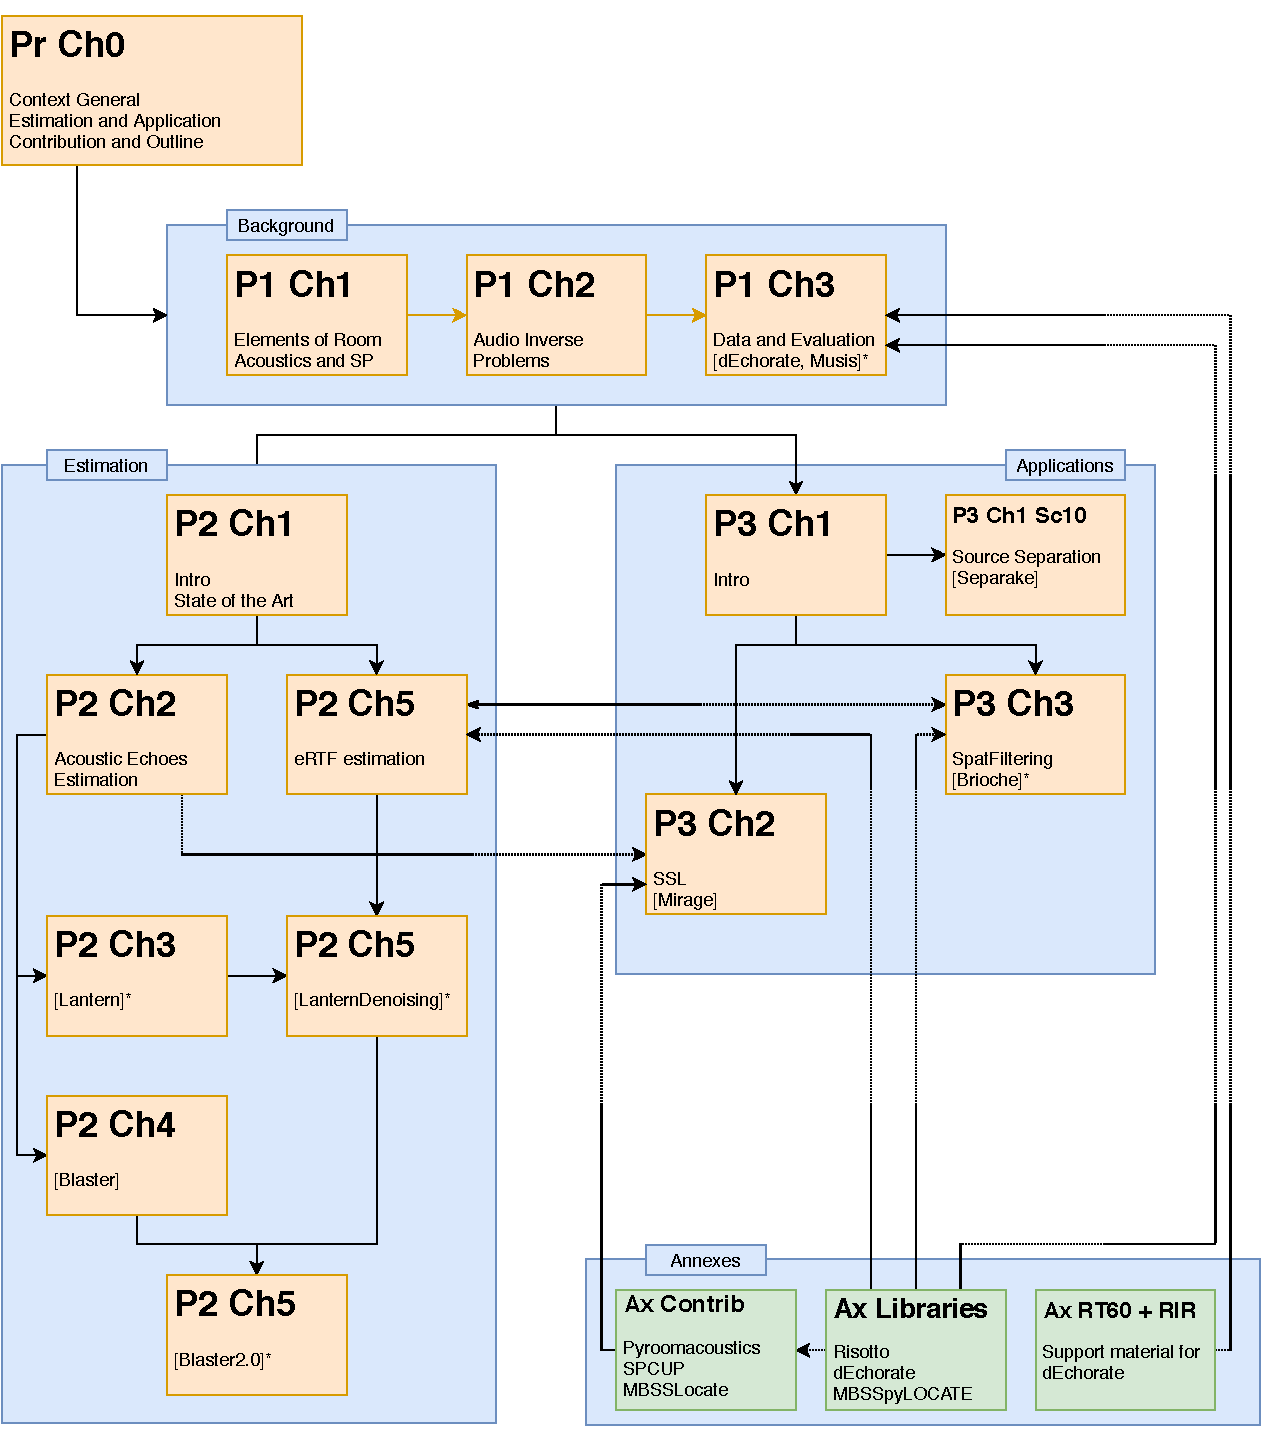
\includegraphics[width=\linewidth]{contents/assets/mindmaps/thesis_mindmap.pdf}
        \end{sidecaption}
\end{figure}


\section{Todos and Notes}

\itodo{Can we use \bison/'s argument (regarding differential cryptanalysis) for a maximal unbalanced Feistel network?}
\miss{Here something is missing}
\todo[inline]{The original todo note withouth changed colours.\newline Here's another line.}

\lipsum[11]\unsure{Is this correct?}\unsure{I'm unsure about also!}
\lipsum[11]\change{Change this!}
\lipsum[11]\info{This can help me in chapter seven!}
\lipsum[11]\plus{What was I thinking?!}
\lipsum[11]
\plus[inline]{The following section needs to be rewritten!}
\lipsum[11]

% \newthoughtpar{Incentives for new Cipher Designs}
% \blindtext

% \section{Section 1}
% \blindtext[3]

% \marginpar{%
%     \footnotesize
%     \vspace{\baselineskip}
%     \vspace*{-7\baselineskip}
%     See \cref{ch:intro} for a detailed explanation of differential cryptanalysis
%     and the problems that appear when trying to bound the differential probability.
% }

% \begin{problem}[Differentials]\label{prob:differentials}
%     \blindtext
% \end{problem}



% \section{Publications}

% During the course of my doctoral studies, I worked on several projects which are not all covered in the remainder of this thesis.
% In particular, these are the following.

% \newthoughtpar{Conference Publications}
% \begin{itemize}
% \item[] \fullfullcite{EC:CLLNW19}, see \cref{ch:bison}.
% %Because \bison/ can only be instantiated with odd block length, we here also give a second instance of the underlying construction: \wisent/.
% %This instance is for the even block length case and basically inherits almost the same security bounds as \bison/.
% \end{itemize}

% \newthoughtpar{Journal Publications}
% \begin{itemize}
%     \item[] \fullfullcite{ToSC:KraLeaWie17}.
%     \item[] \fullfullcite{ToSC:KLSW17}, see \cref{ch:slp}.
%     \item[] \fullfullcite{ToSC:LeaTezWie18}, see \cref{ch:st}.
% \end{itemize}


% \section{Stir of Echoes}

% \blindtext

% \section{Equations}

\begin{align}
    f(x) &= x^2\\
    g(x) &= \frac{1}{x}\\
    F(x) &= \int^a_b \frac{1}{3}x^3
\end{align}


A simple equation:
\[
 f(x)=(x+a)(x+b)
\]
An equation with text:
\begin{equation}
50 \text{ apples} \times 100 \text{ apples} =
\textbf{lots of apples}
\end{equation}
One including subscripts and superscripts:
\[ k_{n+1} = n^2 + k_n^2 - k_{n-1} \]
\section{Greek Letters}
\[ \alpha,  \beta,  \gamma, \Gamma, \pi, \Pi, \phi, \varphi, \mu, \Phi, \xi, \zeta \]
\[ \cos(2\theta\phi) = \cos^2 \theta\phi - \sin^2 \theta\phi \]
\section{Delimiters}
There are many types of delimiters one can use:
\[ ( a ), [ b ], \{ c \}, | d |, \| e \|,
\langle f \rangle, \lfloor g \rfloor,
\lceil h \rceil, \ulcorner i \urcorner \]
See how the delimiters are of reasonable size in these examples
\[
        \left(a+b\right)\left[1-\frac{b}{a+b}\right]=a\,,
\]
\[
        \sqrt{|xy|}\leq\left|\frac{x+y}{2}\right|,
\]
even when there is no matching delimiter
\[
        \int_a^bu\frac{d^2v}{dx^2}\,dx
        =\left.u\frac{dv}{dx}\right|_a^b
        -\int_a^b\frac{du}{dx}\frac{dv}{dx}\,dx.
\]
whereas vector problems often lead to statements such as
\[
        u=\frac{-y}{x^2+y^2}\,,\quad
        v=\frac{x}{x^2+y^2}\,,\quad\text{and}\quad
        w=0\,.
\]
\section{Multiple Fractions}
Typesetting continued fractions is easy:
\[
x = a_0 + \frac{1}{a_1 + \frac{1}{a_2 + \frac{1}{a_3 + a_4}}}
\]
However, as the fractions continue, they get smaller. If you want to keep the size consistent, use the display style; e.g.
\[
  x = a_0 + \frac{1}{\displaystyle a_1
          + \frac{1}{\displaystyle a_2
          + \frac{1}{\displaystyle a_3 + a_4}}}
\]
\section{Arrays}
Arrays of mathematics are typeset using one of the matrix environments as
in
\[
        \begin{bmatrix}
                1 & x & 0 \\
                0 & 1 & -1
        \end{bmatrix}\begin{bmatrix}
                1  \\
                y  \\
                1
        \end{bmatrix}
        =\begin{bmatrix}
                1+xy  \\
                y-1
        \end{bmatrix}.
\]
\[ \begin{pmatrix}
2 & 3 & 4\\
5 & 6 & 7\\
8 & 9 & 10 \end{pmatrix} v = 0 \]
Case statements use cases:
\[
        |x|=\begin{cases}
                x, & \text{if }x\geq 0\,,  \\
                -x, & \text{if }x< 0\,.
        \end{cases}
\]
Many arrays have lots of dots all over the place as in
\[
        \begin{matrix}
                -2 & 1 & 0 & 0 & \cdots & 0  \\
                1 & -2 & 1 & 0 & \cdots & 0  \\
                0 & 1 & -2 & 1 & \cdots & 0  \\
                0 & 0 & 1 & -2 & \ddots & \vdots \\
                \vdots & \vdots & \vdots & \ddots & \ddots & 1  \\
                0 & 0 & 0 & \cdots & 1 & -2
        \end{matrix}
\]
\section{Greek Letters}
\[ \alpha,  \beta,  \gamma, \Gamma, \pi, \Pi, \phi, \varphi, \mu, \Phi, \xi, \zeta \]
\[ \cos(2\theta\phi) = \cos^2 \theta\phi - \sin^2 \theta\phi \]
\section{Delimiters}
\[ ( a ), [ b ], \{ c \}, | d |, \| e \|,
\langle f \rangle, \lfloor g \rfloor,
\lceil h \rceil, \ulcorner i \urcorner \]
\section{Accents}
Mathematical accents are performed by a short command with one
argument, such as
\[
        \tilde f(\omega)=\frac{1}{2\pi}
        \int_{-\infty}^\infty f(x)e^{-i\omega x}\,dx\,,
\]
or
\[
        \dot{\vec \omega}=\vec r\times\vec I\,.
\]
\section{Multiline equations and aligned environments}
New lines (\\ ) do not work in equation environments. To achieve alignment of equations, use the aligned  package to produce multiline aligned math, such as:
\newline

% \[
% \begin{center}
% \begin{aligned}
% $F$ ={} & $\{F_{x} \in  F_{c} : (|S| > |C|)$ \\
%       & $\cap (\mathrm{minPixels}  < |S| < \mathrm{maxPixels})$ \\
%       & $\cap (|S_{\mathrm{conected}}| > |S| - \epsilon) $\}
% \end{aligned}
% \end{center}
% \]

% \newline

% and also:

% \newline
% \[
% \begin{center}
% \begin{aligned}
% $A_0$ & $=   \frac{1}{(\alpha+t_x)^{r+s+x}}{}_2 F_1\left( r+s+x,x+1;r+s+x+1;\frac{\alpha-\beta}{\alpha + t_x} \right) $\\
% & $\quad - \frac{1}{(\alpha+T)^{r+s+x}}{}_2 F_1\left( r+s+x,x+1;r+s+x+1;\frac{\alpha-\beta}{\alpha + T} \right),$
% \end{aligned}
% \end{center}
% \]
% \newline

\textbf{Note}: the above multiline equations have math mode defined per line, not globally at the equation level.
\section{Theorems and sets}

% \newtheorem{theorem}{Theorem}
% \newtheorem{corollary}[theorem]{Corollary}
% \newtheorem{lemma}[theorem]{Lemma}
% \newtheorem{definition}[theorem]{Definition}

\begin{theorem}
For any nonnegative integer $n$, we have
$$(1+x)^n = \sum_{i=0}^n {n \choose i} x^i$$
\end{theorem}
The Taylor series expansion for the function $e^x$ is given by
\begin{equation}
e^x = 1 + x + \frac{x^2}{2} + \frac{x^3}{6} + \cdots = \sum_{n\geq 0} \frac{x^n}{n!}
\end{equation}
\[ \forall x \in X, \quad \exists y \leq \epsilon \]
\[ \frac{n!}{k!(n-k)!} = \binom{n}{k} \]
\begin{theorem}
For any sets $A$, $B$ and $C$, we have
$$ (A\cup B)-(C-A) = A \cup (B-C)$$
\end{theorem}

\blindtext
\blinditemize

\blindtext
\blindenumerate

\blindtext
\blinddescription
\input{contents/main_matter/chapter1_intro}

\begin{fullwidth}
    \part{Pages of Acoustics and Audio Signal Processing}
\end{fullwidth}
\input{contents/main_matter/chapter2_acoustics}
\input{contents/main_matter/chapter3_processing}

% \begin{fullwidth}
% \part{Acoustic Echoes Retrieval}
% \end{fullwidth}
% \input{contents/main_matter/chapter3_aer}
% \input{contents/main_matter/chapter4_lantern}
% \input{contents/main_matter/chapter5_blaster}

% \begin{fullwidth}
% \part{Echo-aware Application}
% \end{fullwidth}
% \input{contents/main_matter/chapter6_applications}
% \input{contents/main_matter/chapter7_mirage}
% \input{contents/main_matter/chapter8_brioche}

% \begin{fullwidth}
% \part{Epilogue}
% \end{fullwidth}
% \chapter{Conclusion}\label{ch:conclusion}
\openepigraph{But at the laste, every thing hath ende}{Geoffrey Chaucer}
Since the development of the \DES/ and \AES/, our understanding of secure designs for encryption schemes has greatly evolved.
In particular in the area of symmetric cryptography, we are today, after more than 40 years of research, able to design very efficient ciphers, which we firmly believe to be secure -- with the \AES/ being the prime example withstanding 20 years of cryptanalysis.
Our progress pushed efficiency bounds further and further, especially within the trend of lightweight cryptography.

However the time may has come where we should shift our focus to improving security arguments for new designs -- because the improvement since the development of bounds for differential and linear cryptanalysis seems marginal.
We see this thesis, specifically the first part on security arguments, as a step in this direction.
With our block cipher instances \bison/ and \wisent/ we are for the first time able to give precise bounds on the \emph{differential} instead of only on differential trails.
This initial result may lead to further investigation of alternative constructions for block ciphers.
An interesting question in this direction is if a construction can be found which exhibits similar good properties with respect to linear cryptanalysis.
A second worthwhile direction is the study of unbalanced Feistel networks which seem to be related to the \WSN/ construction.

Apart from our results on differential cryptanalysis, our study of the \ACT/ revealed a connection between differential-linear cryptanalysis and previously studied properties of Boolean functions.
In our opinion the most interesting observation, from a cryptanalytic perspective, is that the decryption function might be weaker than the encryption against differential-linear attacks.
This result implies future analysis has to be extended in this direction.
From a more theoretical point of view, it is interesting that vectorial Boolean functions exhibit a lower bound for the absolute indicator, while for Boolean functions it seems to be a hard problem finding such a lower bound.
Overall, our results on this new connection contribute to a further understanding of differential-linear cryptanalysis.

In the second part of the thesis, we concentrated on automated tools for the design and analysis of block ciphers.
Our main result here was the conceptual simple algorithm for propagating subspaces through an iterative round function.
Despite the underlying simple idea, this algorithm turns out to be useful not only for one application.
For its original purpose, we use \textsc{Compute Trail} to algorithmically bound the longest subspace trail through an \SPN/ cipher and thus construct an algorithmic security argument against this recent type of attack.

However, besides the study of single attacks, a more principle task is to extend a distinguishing attack into a key recovery.
Especially when such an extension is possible over some rounds, it might make the difference between a cipher with a thin security margin and a broken one.
Thus, while being a very important part of cryptanalysis, finding key recovery strategies remains a highly manual, and thus error prone, task.
As discussed in the last chapter, our subspace trail algorithm may be used in an automatisation approach for exactly this problem -- albeit working out the exact techniques for such an automated key recovery remains to be done.

Apart from these possibilities for automated tools discussed in this thesis, a different application are cryptanalysis techniques based on \MILPp/.
We only briefly mentioned \MILPp/ for bounding the number of active S-boxes.
However, they have by now a broad spectrum of use cases, \eg/ for finding differential or linear trails, for finding division properties or similar.
All these applications have the same basic process that needs the cipher under scrutiny and the analysis technique to be modeled as an instance of the specific programming style, \ie/ as a \MILP/.
The needed building blocks for these models are known for every typical part used in ciphers, still the cryptanalyst has to assemble the models manually.
Again this is a tedious and error prone task which could easily be automated.
The development of such a \MILP/ compiler (or similarly a SAT compiler for constrained programming models) quite likely requires techniques from programming languages and compiler theory.
It seems to be an interesting problem to work on.

Finding the best representation of a cipher for these models (both for \MILPp/ and SAT) is another problem which yet remains unsolved.
This occurs especially when modeling the nonlinear S-boxes, for which different approaches exist: broadly speaking one could model the S-box in full detail, or try to pre-optimise the model on a varying level.
Similar to the XOR count optimisations it is then unclear, how much pre-optimisation helps in the end and what level of optimisation restricts the solver too much for its own optimisation strategies.



\begin{fullwidth}
\printbibliography{}
\end{fullwidth}

\cleardoublepage{}

%%%% APPENDIX

\begin{appendices}
\chapter{Mindmaps}

\Blindtext
\chapter{RIR and RT60 measurements}

\Blindtext
\end{appendices}

\end{document}
